
\title{Addendum to the Report on the ITER Clite Shutdown Dose rate Calculations}
\author{
  Andrew Davis \\
  Department of Engineering Physics\\
  College of Engineering \\
  The University of Wisconsin-Madison\\
  Madison, Wisconsin, 53706, \underline{USA}
  \and
  Mohamed Sawan \\
  Department of Engineering Physics\\
  College of Engineering \\
  The University of Wisconsin-Madison\\
  Madison, Wisconsin, 53706, \underline{USA}
  \and
  Paul P. H. Wilson \\
  Department of Engineering Physics\\
  College of Engineering \\
  The University of Wisconsin-Madison\\
  Madison, Wisconsin, 53706, \underline{USA}
  \and
  Elliott Biondo \\
  Department of Engineering Physics\\
  College of Engineering \\
  The University of Wisconsin-Madison\\
  Madison, Wisconsin, 53706, \underline{USA}
  \and
  Ahmad Ibrahim \\
  Radiation Transport Group\\
  Oak Ridge National Laboratory \\
  P.O. Box 2008 \\
  Oak Ridge, Tennessee 37831, \underline{USA}
  \and
  Patrick Shriwise \\
  Department of Engineering Physics\\
  College of Engineering \\
  The University of Wisconsin-Madison\\
  Madison, Wisconsin, 53706, \underline{USA}
  \and
  Edward Marriott\\
  Department of Engineering Physics\\
  College of Engineering \\
  The University of Wisconsin-Madison\\
  Madison, Wisconsin, 53706, \underline{USA}
}

\date{\today}

\documentclass[12pt]{article}
\usepackage{times}
\usepackage{graphicx}
\usepackage{longtable}
\usepackage[acronym]{glossaries}
\usepackage[a4paper, portrait, margin=0.5in]{geometry}
\usepackage[table]{xcolor}
\usepackage[nottoc,numbib]{tocbibind}
\usepackage{subcaption}
\usepackage{multirow}
\usepackage{draftwatermark}
\usepackage[hidelinks]{hyperref}

\SetWatermarkText{DRAFT}
\SetWatermarkScale{1}

%% define this page left blank
\newcommand*{\blankpage}{%
\vspace*{\fill}
\begin{center}
 \centering \textbf{This page intentionally left blank}
\end{center}
\vspace{\fill}}

%% to get lof in toc
\renewcommand{\listoffigures}{\begingroup
\tocsection
\tocfile{\listfigurename}{lof}
\endgroup}

%% to get lot in toc
\renewcommand{\listoftables}{\begingroup
\tocsection
\tocfile{\listtablename}{lot}
\endgroup}

\begin{document}
\maketitle
\newpage
\tableofcontents
\newpage
\listoffigures
\newpage
\listoftables
\newpage
\section{Introduction}
The original report \cite{iter_sdr_report} contained results for the baseline
ITER SA-2 irradiation scenario, included in this report are the two remaining
scenarios a reduced 5 year scenario and a 10 year irradation scenario. 
\\
\\
The models and paramters for transport and activation are entirely unchanged 
and only differ by the irradiation scenario used, which is detailed in Section
\ref{sec:irradiation_scenario}
\newpage
\section{Irradiation Scenarios}
\label{sec:irradiation_scenario}
The following irradiation scenarios are the standard SA-2 scenario and 
two reduced versions of the ITER SA-2.
irradiation scenarios \cite{sa2_irradiation}. 
\subsection{ITER SA-2 Full}
\begin{table}[ht!]
   \begin{tabular}{| l | c | c | c |}
      \hline 
      Irradiation Period & Neutron Power (MW) & Source Normalisation (n/s) &  Relative Strength \\
      \hline
      2 Years & 2.7 & $1.061\times10^{17}$ & 0.0053 \\
      10 Years & 20.6 & $8.517\times10^{17}$ & 0.0412 \\
      0.667 Years & 0.0 & 0.0 & 0.0 \\
      1.325 Years & 41.5 & $1.643\times10^{18}$ & 0.0830 \\
      \cellcolor{blue!25} 3920 Seconds & \cellcolor{blue!25} 0.0 & \cellcolor{blue!25} 0.0 & \cellcolor{blue!25} 0.0 \\
      \cellcolor{blue!25} \cellcolor{blue!25} 400 Seconds & \cellcolor{blue!25} 500.0 & \cellcolor{blue!25} $1.973\times10^{19}$ & \cellcolor{blue!25} 1.0  \\
      \cellcolor{green!25} 3920 Seconds & \cellcolor{green!25} 0.0 & \cellcolor{green!25} 0.0 &\cellcolor{green!25} 0.0 \\
      \cellcolor{green!25} 400 Seconds & \cellcolor{green!25} 700.0 & \cellcolor{green!25} $2.772\times10^{19}$ &\cellcolor{green!25} 1.4 \\
      \hline
\end{tabular}
\caption{The table shows the SA-2 scenario for irradiation, note the
         cells in \textcolor{blue!25}{blue} are repeated 17 times
         and the cells in \textcolor{green!25}{green} are repeated 3
         times.}
\label{tab:irrad_scenario}
\end{table}
\subsection{ITER SA-2 10 year}
\begin{table}[ht!]
   \begin{tabular}{| l | c | c | c |}
      \hline 
      Irradiation Period & Neutron Power (MW) & Source Normalisation (n/s) &  Relative Strength \\
      \hline
      2 Years & 2.7 & $1.061\times10^{17}$ & 0.0053 \\
      5 Years & 20.6 & $8.517\times10^{17}$ & 0.0412 \\
      0.667 Years & 0.0 & 0.0 & 0.0 \\
      1.325 Years & 41.5 & $1.643\times10^{18}$ & 0.0830 \\
      \cellcolor{blue!25} 3920 Seconds & \cellcolor{blue!25} 0.0 & \cellcolor{blue!25} 0.0 & \cellcolor{blue!25} 0.0 \\
      \cellcolor{blue!25} \cellcolor{blue!25} 400 Seconds & \cellcolor{blue!25} 500.0 & \cellcolor{blue!25} $1.973\times10^{19}$ & \cellcolor{blue!25} 1.0  \\
      \cellcolor{green!25} 3920 Seconds & \cellcolor{green!25} 0.0 & \cellcolor{green!25} 0.0 &\cellcolor{green!25} 0.0 \\
      \cellcolor{green!25} 400 Seconds & \cellcolor{green!25} 700.0 & \cellcolor{green!25} $2.772\times10^{19}$ &\cellcolor{green!25} 1.4 \\
      \hline
\end{tabular}
\caption{The table shows the SA-2 10 year scenario for irradiation, note the
         cells in \textcolor{blue!25}{blue} are repeated 17 times
         and the cells in \textcolor{green!25}{green} are repeated 3
         times.}
\end{table}
\subsection{ITER SA-2 5 year}
\begin{table}[ht!]
   \begin{tabular}{| l | c | c | c |}
      \hline 
      Irradiation Period & Neutron Power (MW) & Source Normalisation (n/s) &  Relative Strength \\
      \hline
      2 Years & 2.7 & $1.061\times10^{17}$ & 0.0053 \\
      0.667 Years & 0.0 & 0.0 & 0.0 \\
      1.325 Years & 41.5 & $1.643\times10^{18}$ & 0.0830 \\
      \cellcolor{blue!25} 3920 Seconds & \cellcolor{blue!25} 0.0 & \cellcolor{blue!25} 0.0 & \cellcolor{blue!25} 0.0 \\
      \cellcolor{blue!25} \cellcolor{blue!25} 400 Seconds & \cellcolor{blue!25} 500.0 & \cellcolor{blue!25} $1.973\times10^{19}$ & \cellcolor{blue!25} 1.0  \\
      \cellcolor{green!25} 3920 Seconds & \cellcolor{green!25} 0.0 & \cellcolor{green!25} 0.0 &\cellcolor{green!25} 0.0 \\
      \cellcolor{green!25} 400 Seconds & \cellcolor{green!25} 700.0 & \cellcolor{green!25} $2.772\times10^{19}$ &\cellcolor{green!25} 1.4 \\
      \hline
\end{tabular}
\caption{The table shows the SA-2 5 year scenario for irradiation, note the
         cells in \textcolor{blue!25}{blue} are repeated 17 times
         and the cells in \textcolor{green!25}{green} are repeated 3
         times.}
\end{table}

\newpage
\section{Shutdown Photon Transport Results}
\subsection{B$_4$C}
\begin{figure}[ht!]
\centering
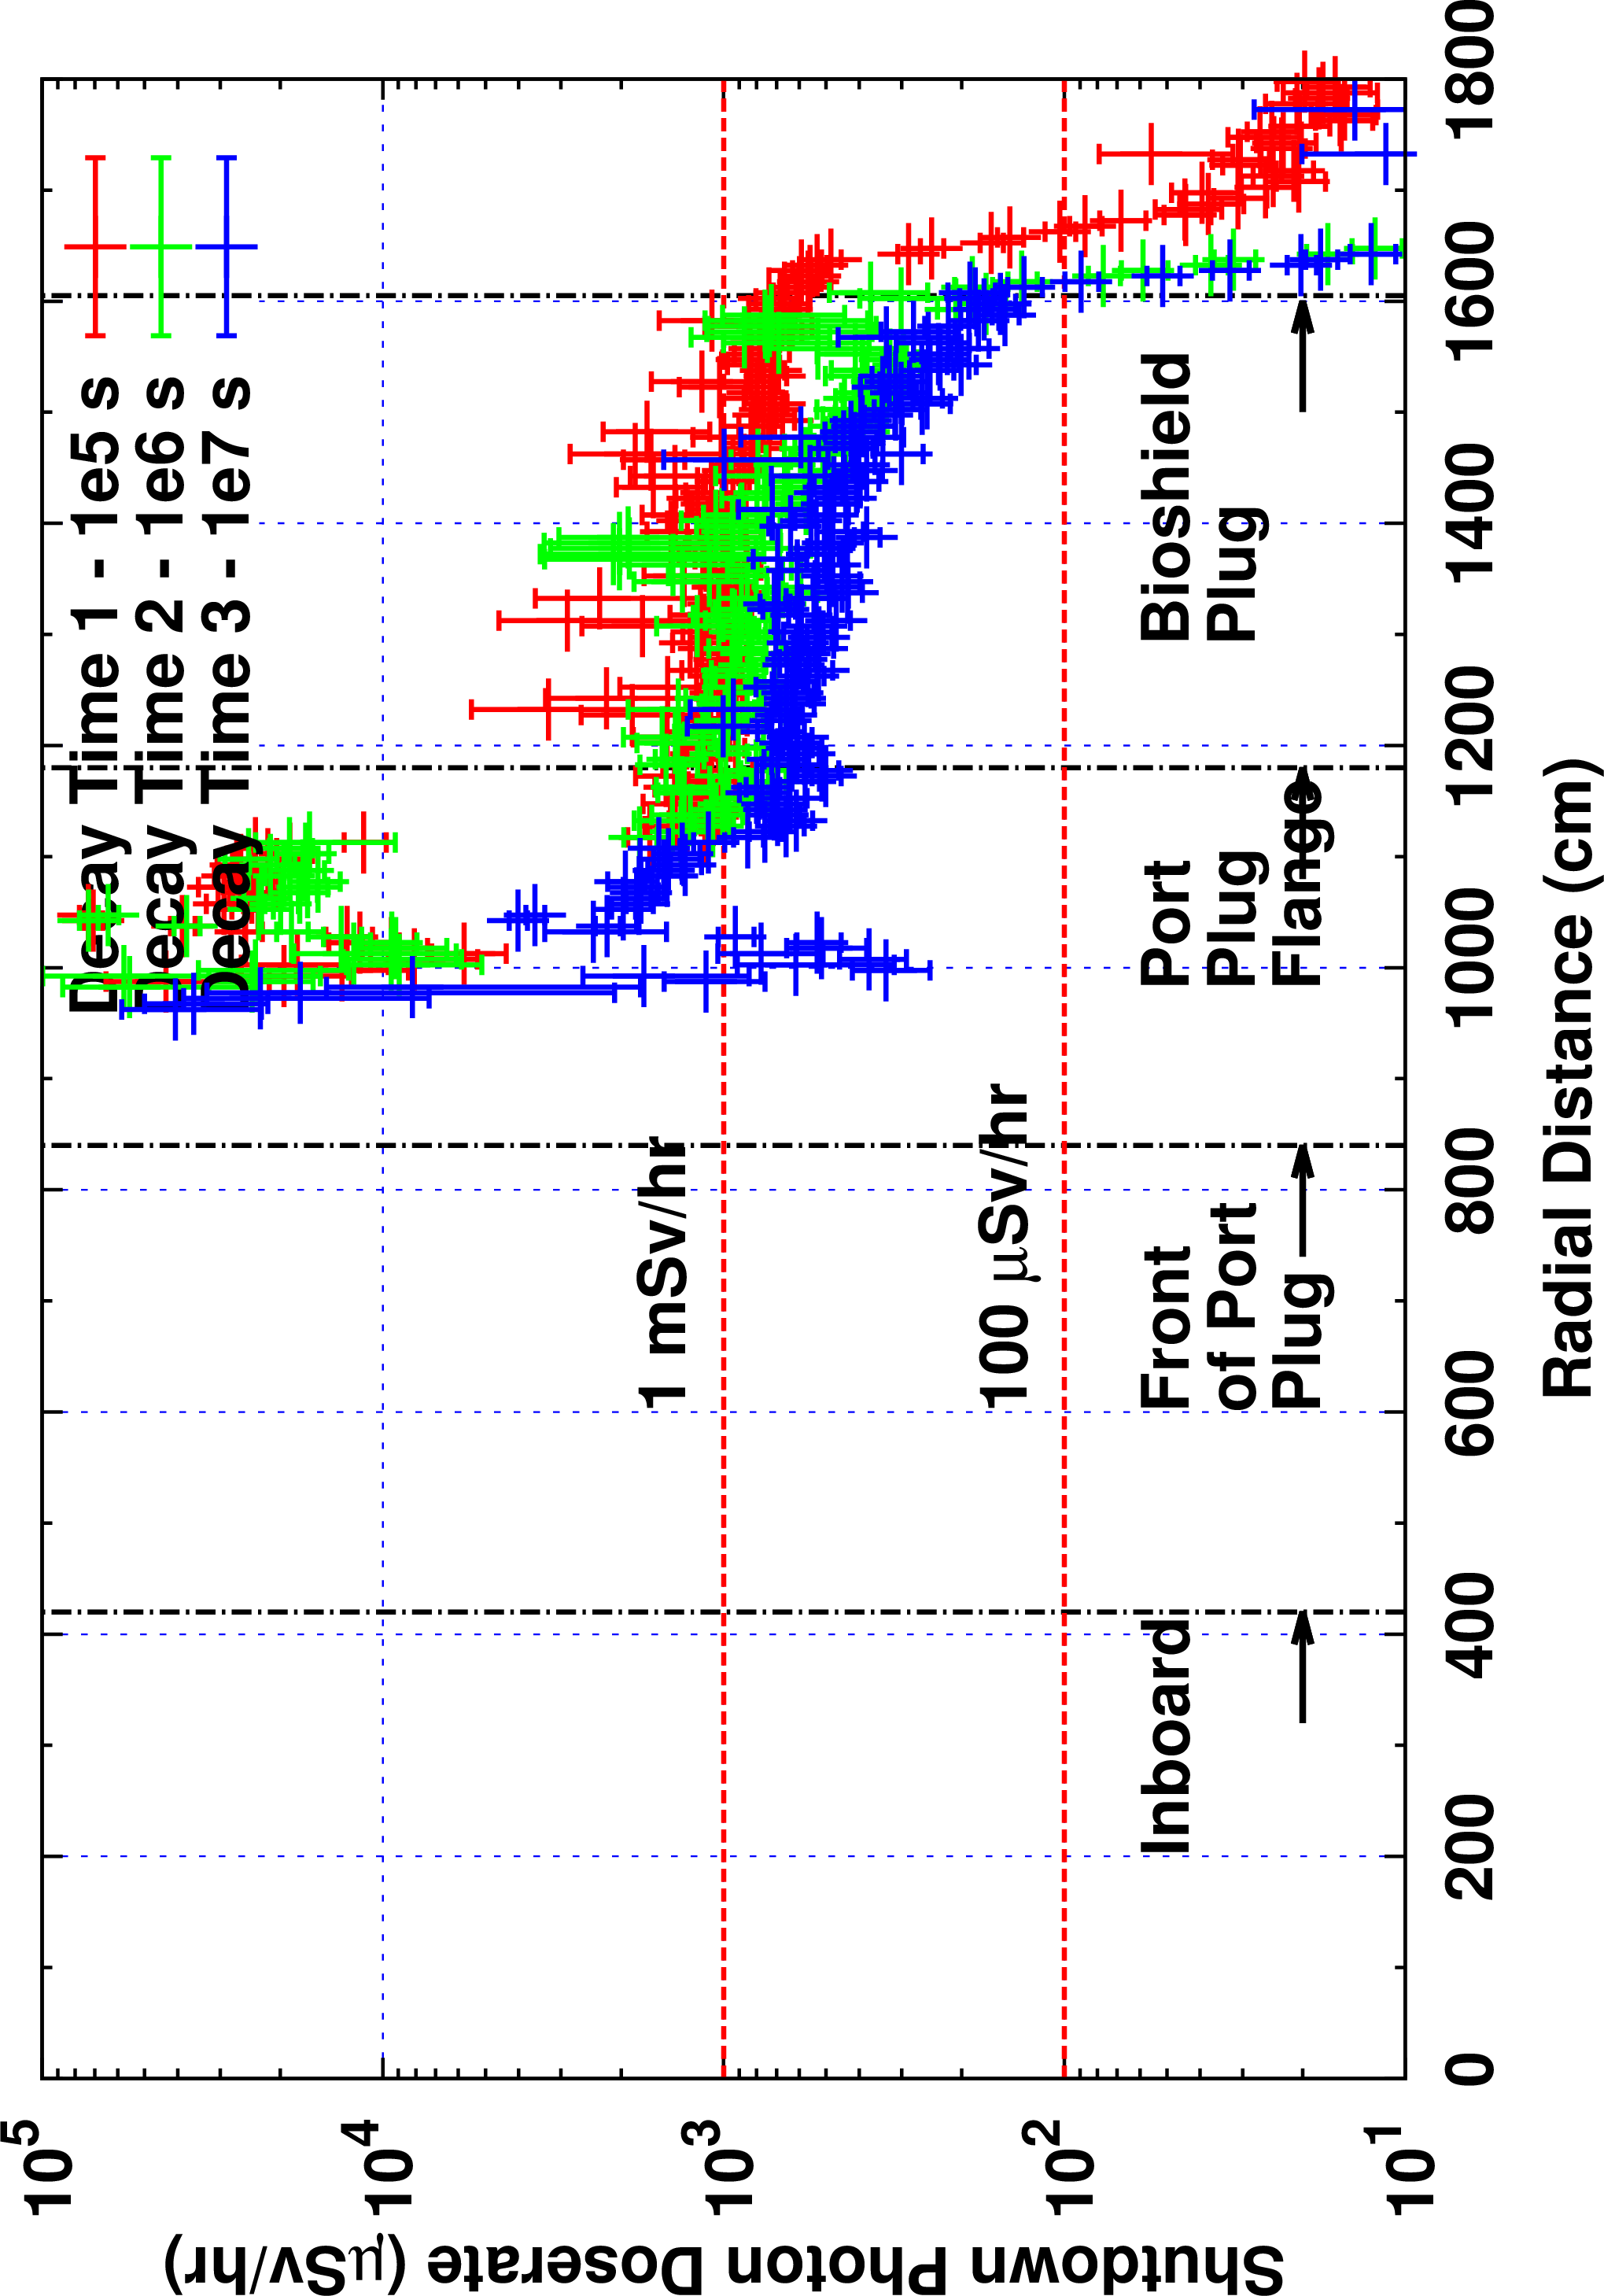
\includegraphics[clip,scale=0.12,angle=-90]{../plots/photon_lineout/5yr/b4c_5yr.png}
\caption{Total dose rate line from 0,0,60 to 1800,0,60 cm for the 5 year irradiation}
\label{fig:photons_5y_b4c_dose}
\end{figure}
\begin{figure}[ht!]
\centering
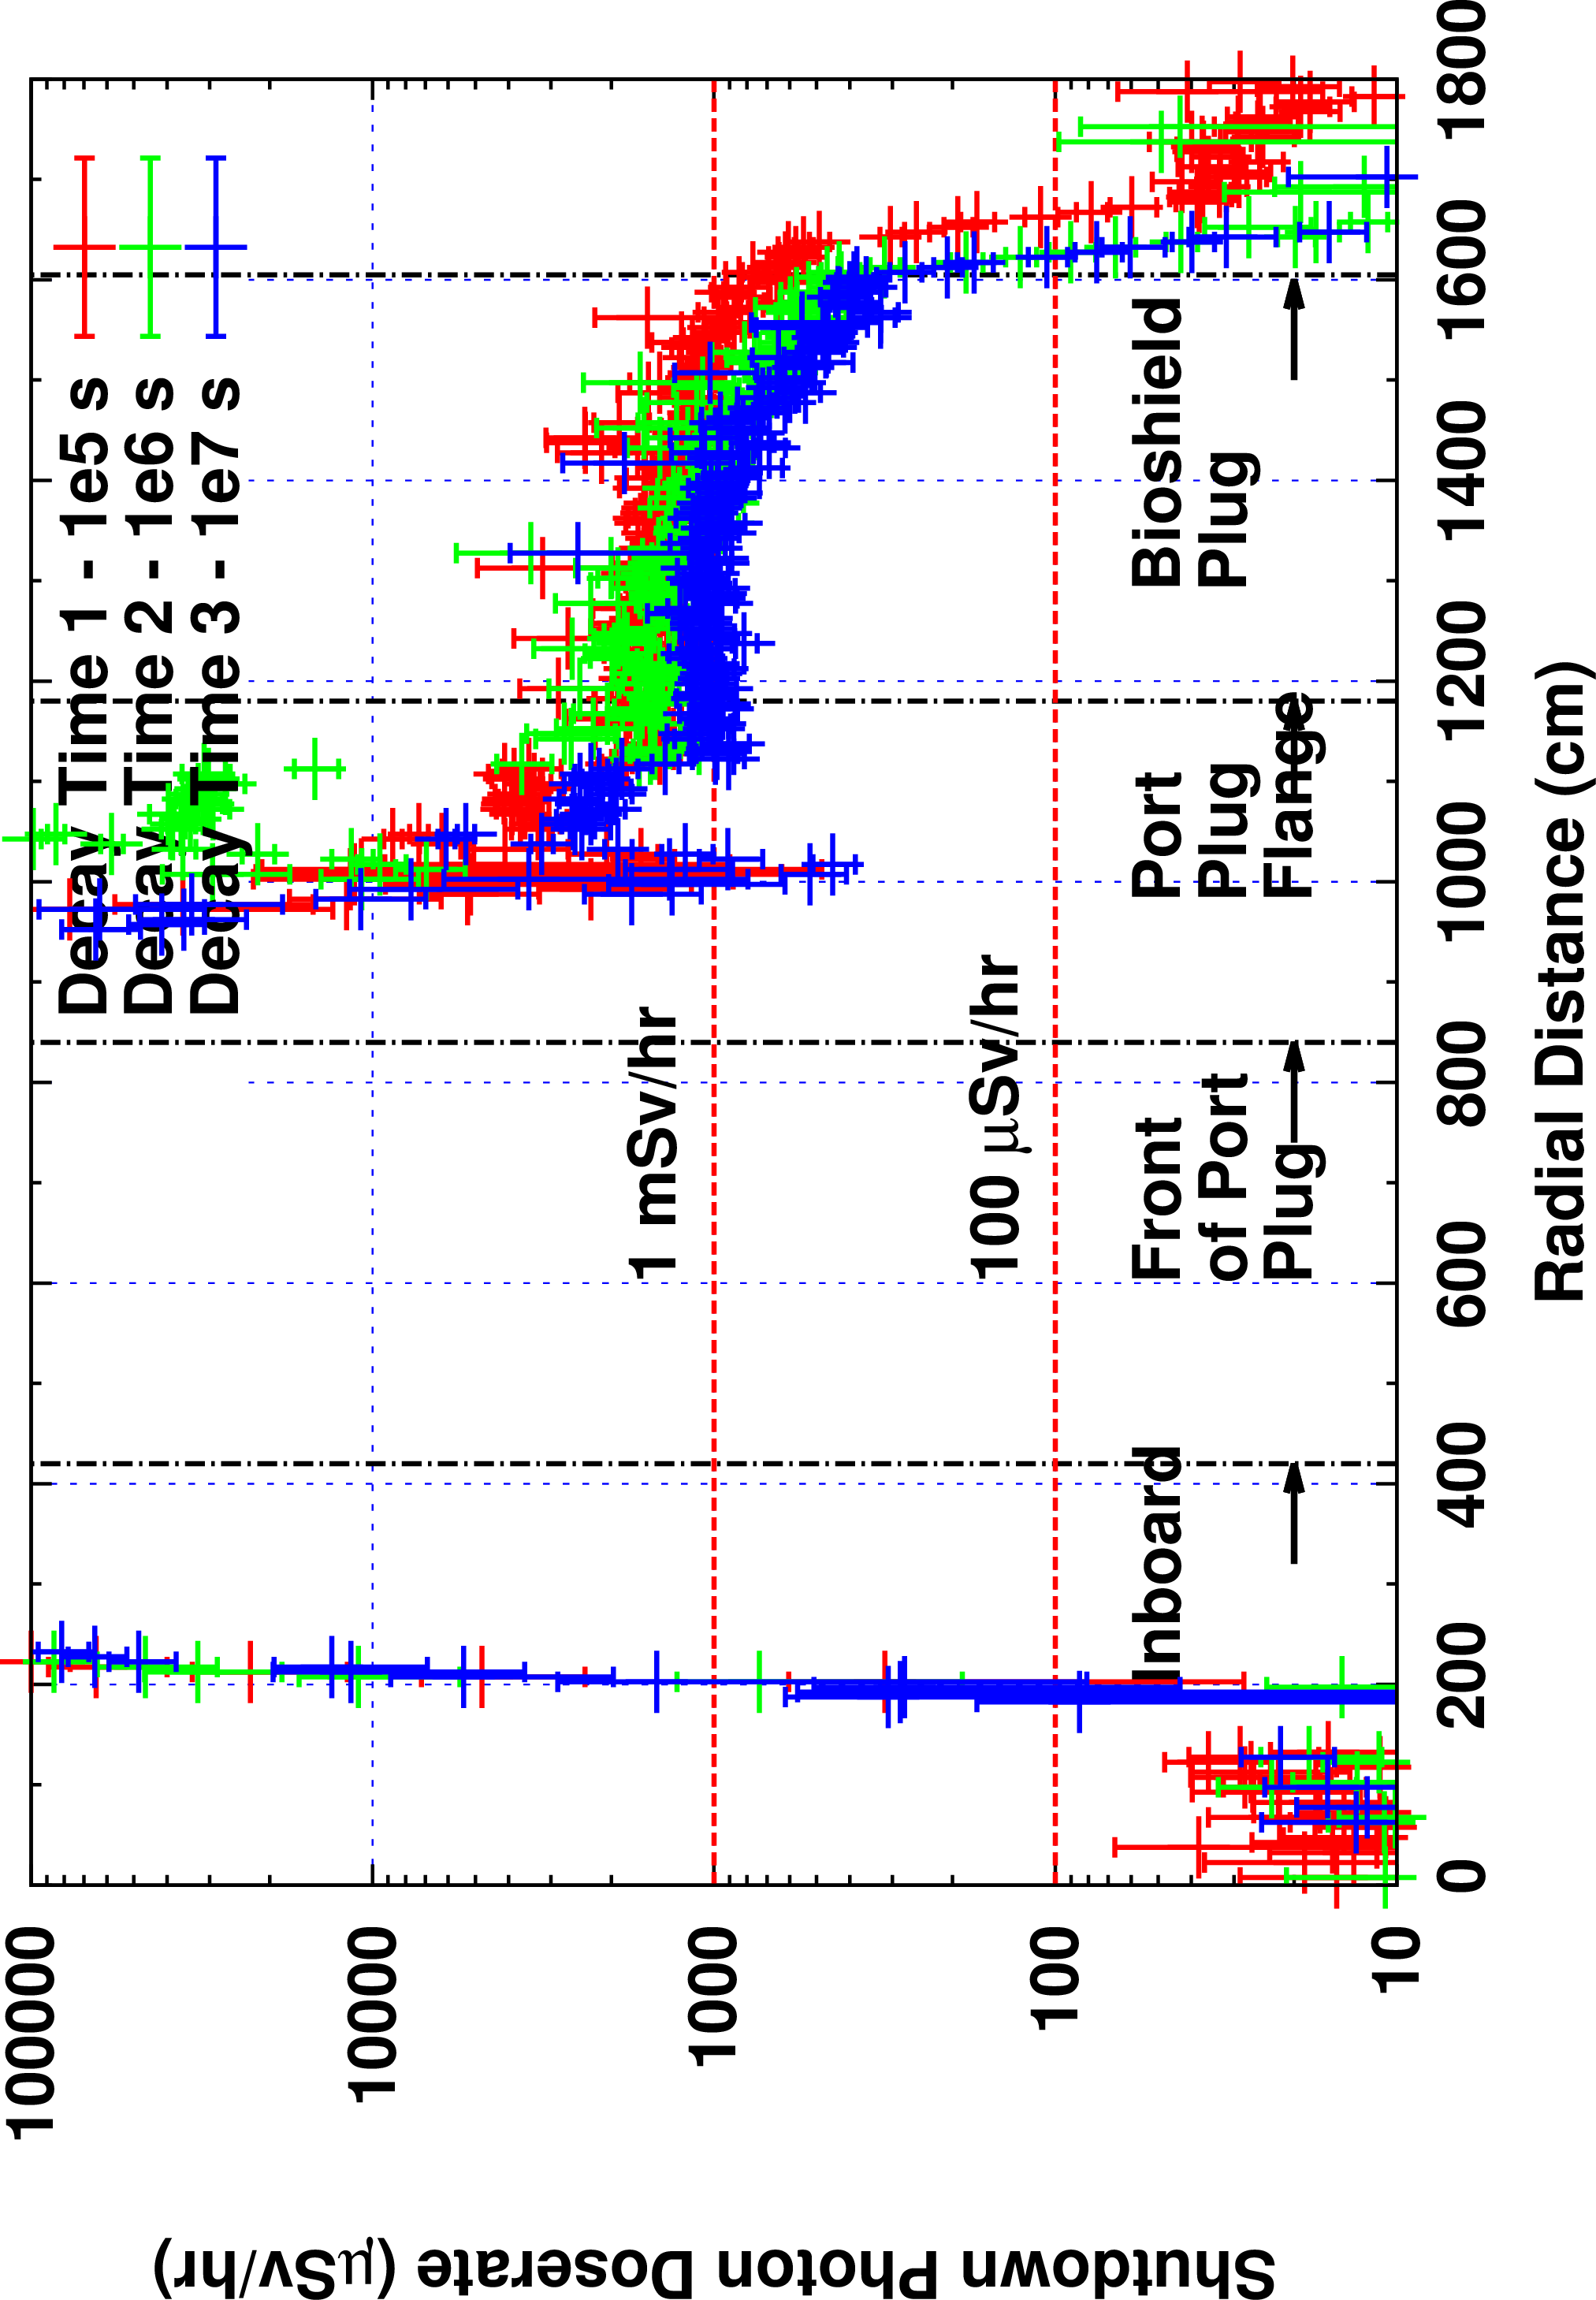
\includegraphics[clip,scale=0.12,angle=-90]{../plots/photon_lineout/10yr/b4c_10yr.png}
\caption{Total dose rate line line from 0,0,60 to 1800,0,60 cm for the 10 year irradiation}
\label{fig:photons_10y_b4c_dose}
\end{figure}
\clearpage
\newpage
\subsection{No B$_4$C}
\begin{figure}[ht!]
\centering
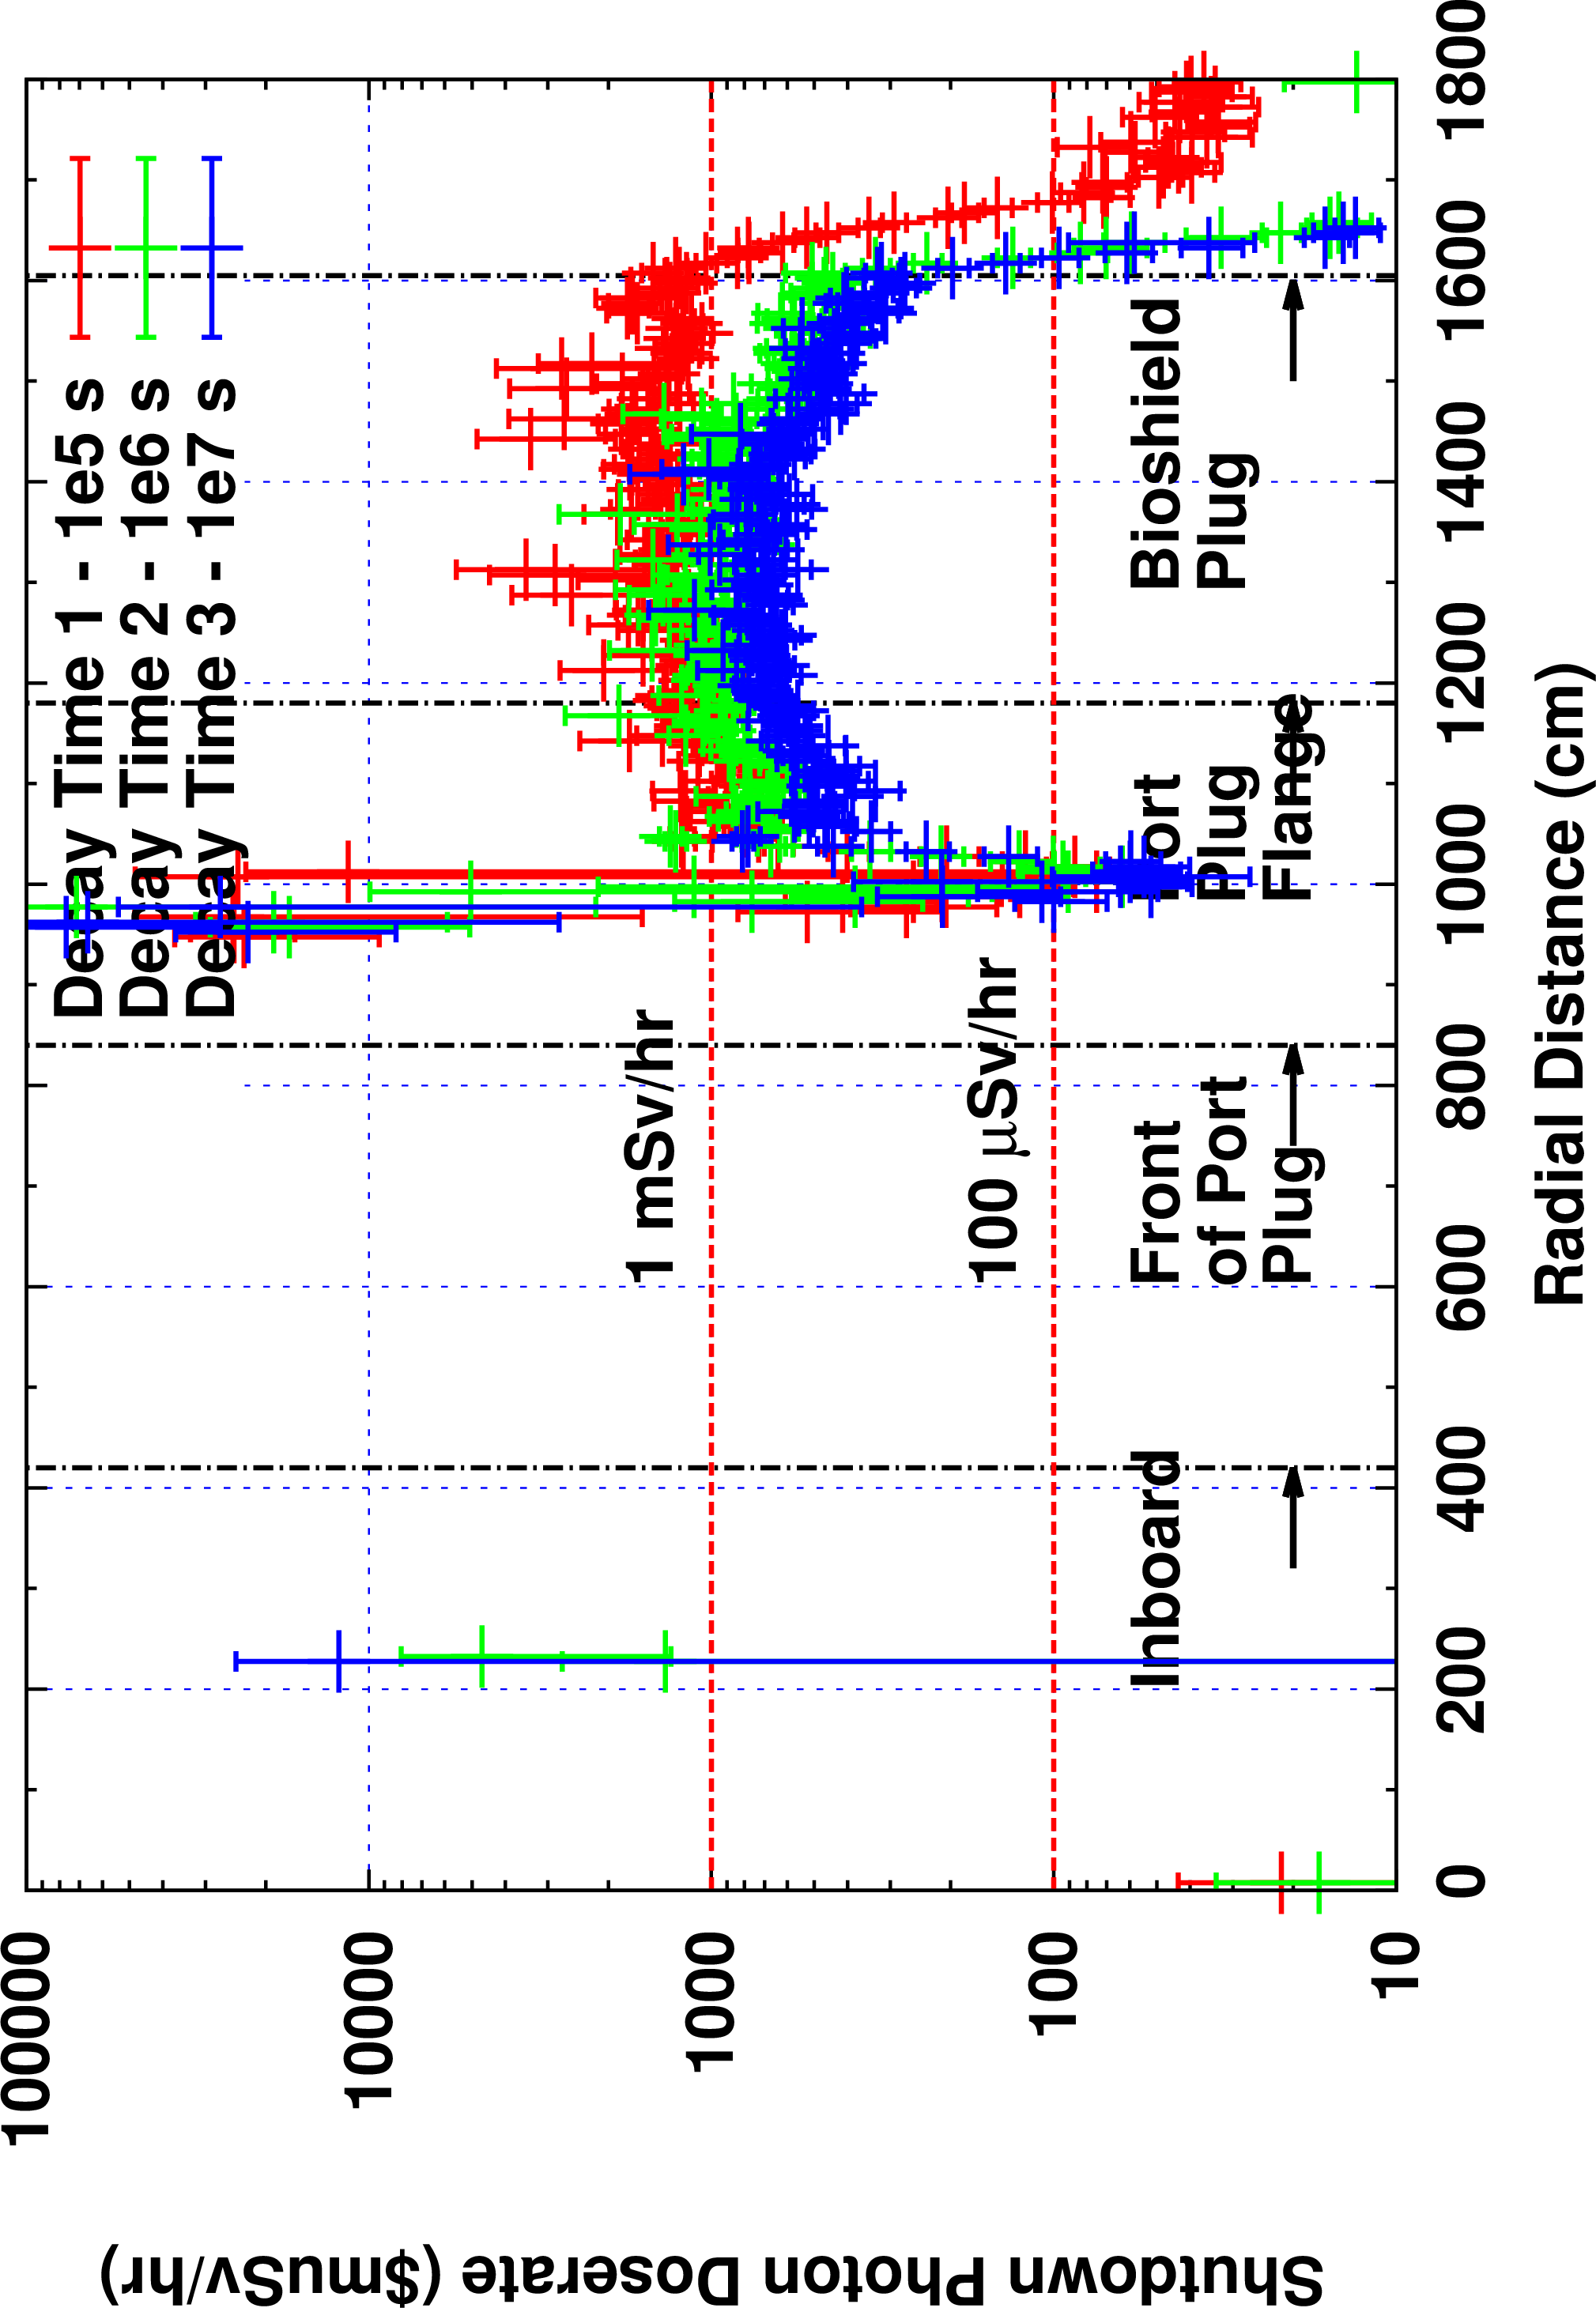
\includegraphics[clip,scale=0.12,angle=-90]{../plots/photon_lineout/5yr/no-b4c_5yr.png}
\caption{Total dose rate line from 0,0,60 to 1800,0,60 cm for the 5 year irradiation}
\label{fig:photons_5y_nob4c_dose}
\end{figure}
\begin{figure}[ht!]
\centering
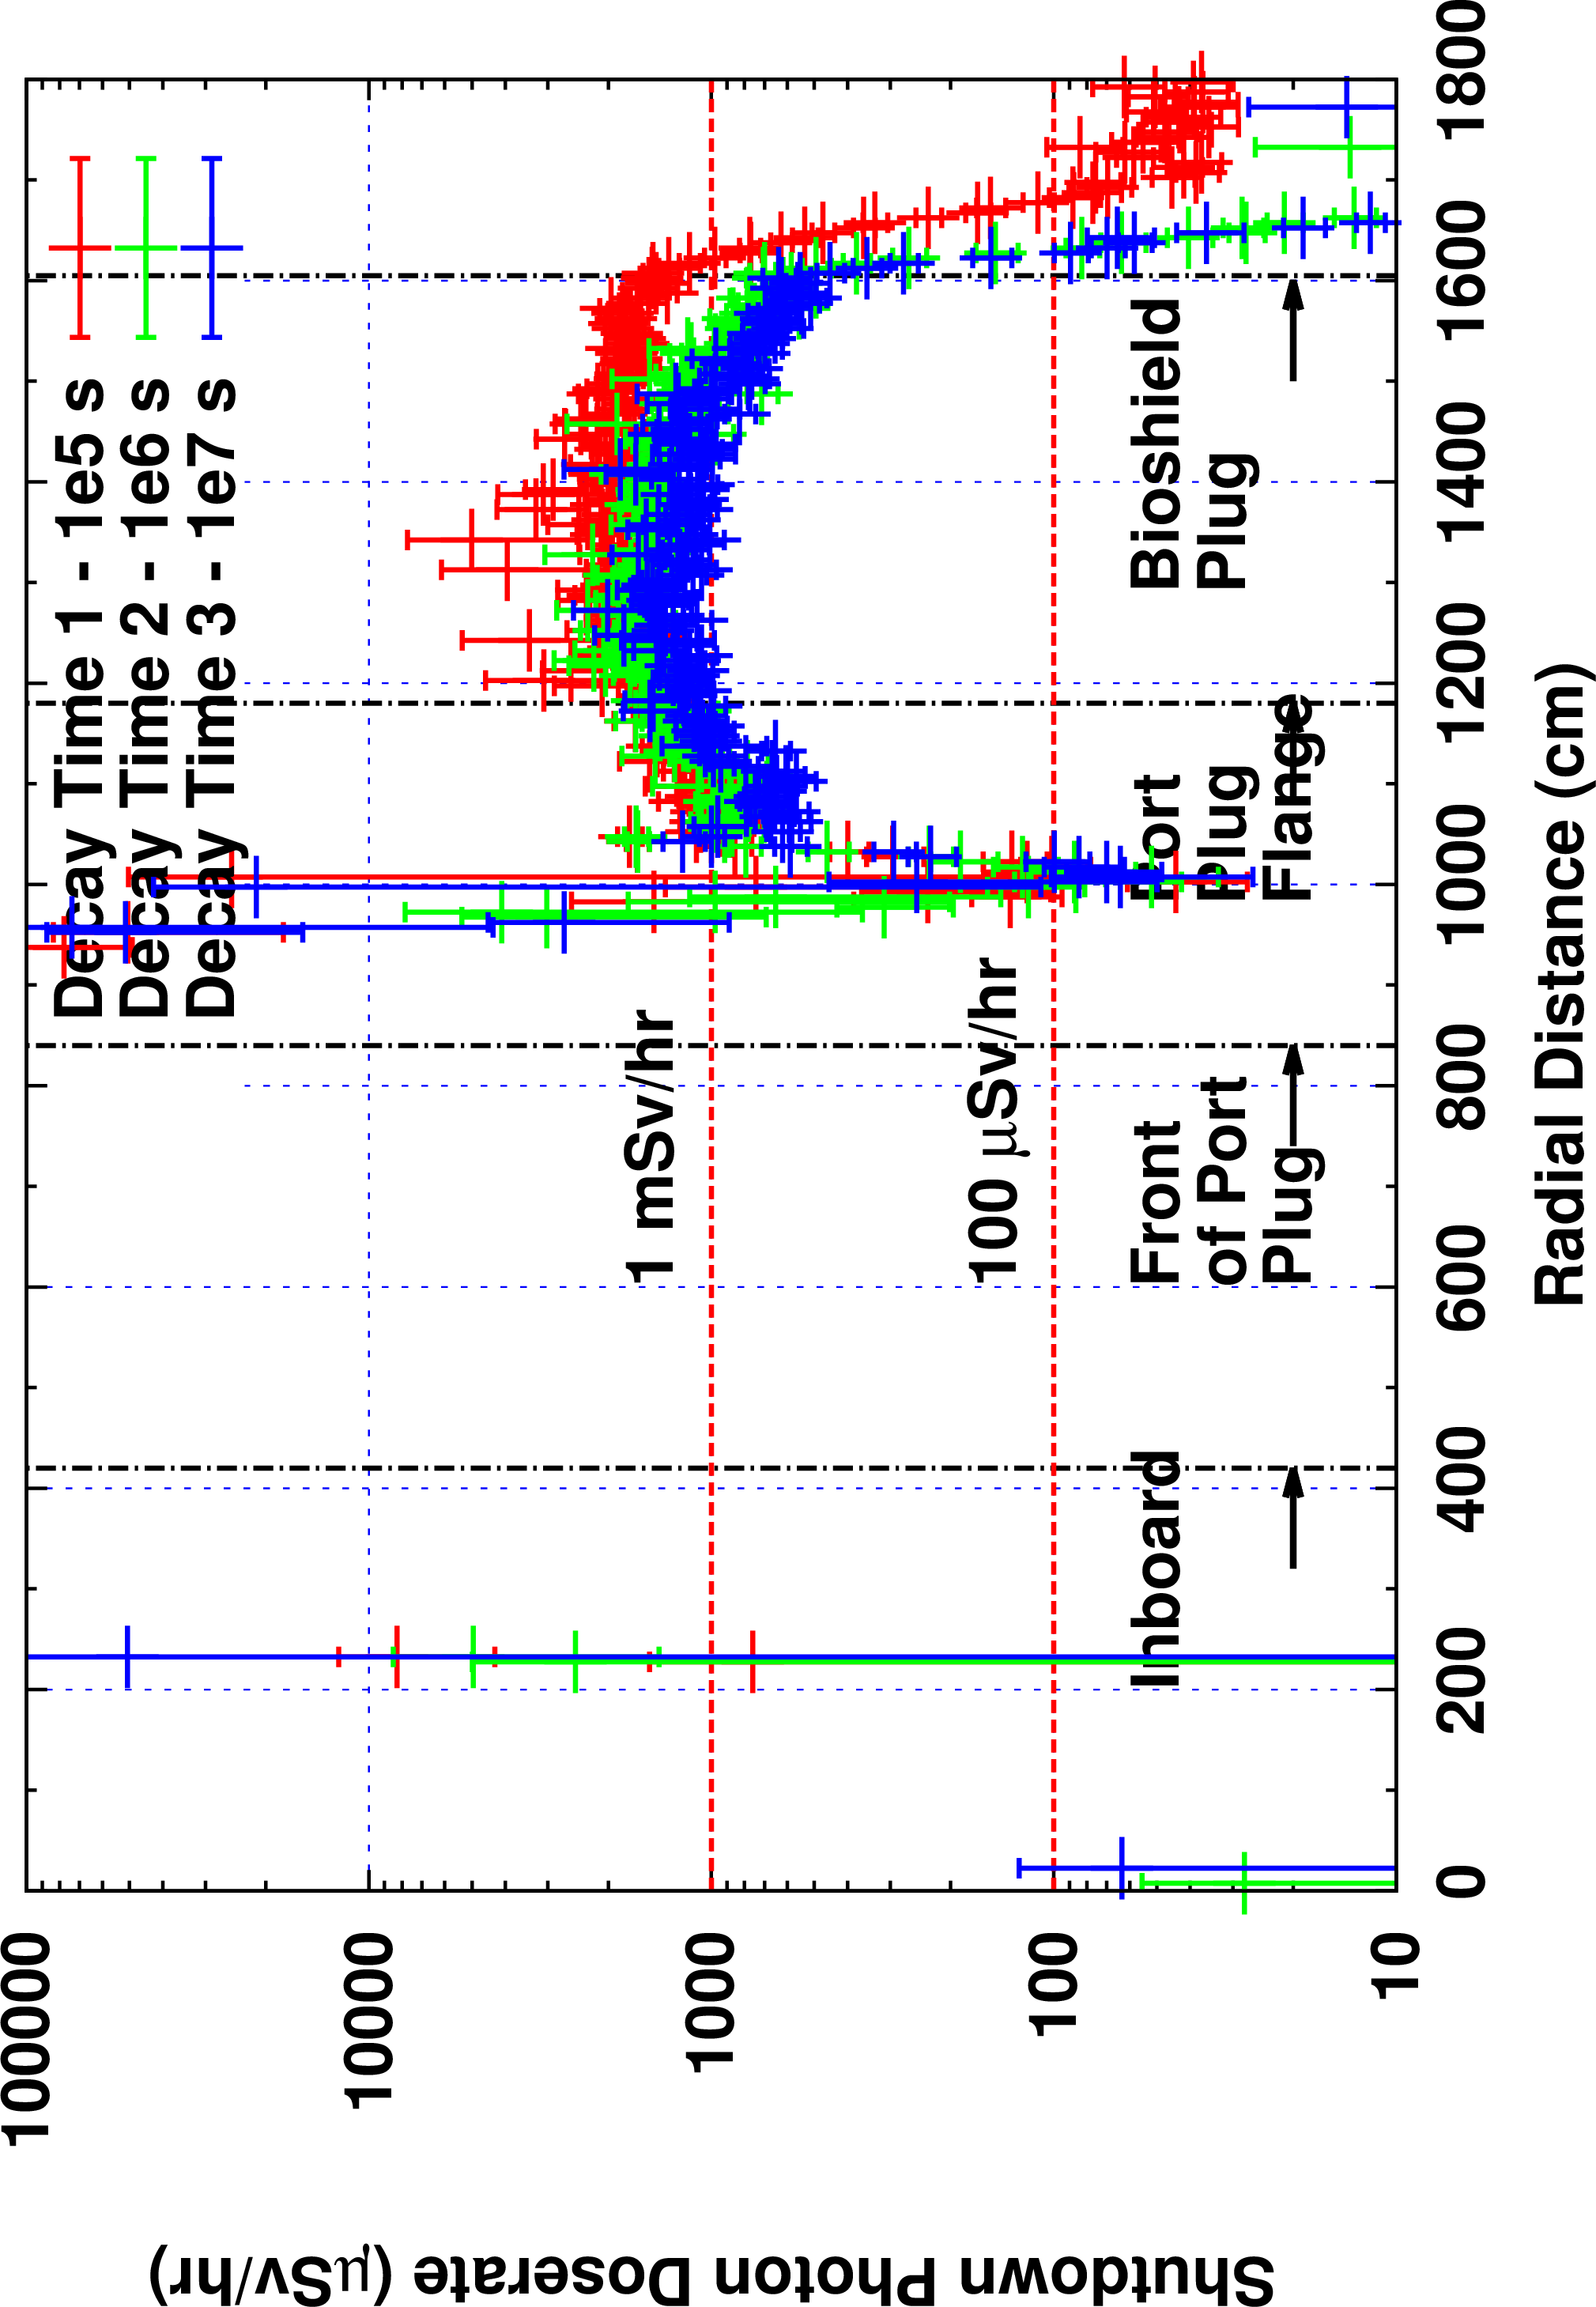
\includegraphics[clip,scale=0.12,angle=-90]{../plots/photon_lineout/10yr/no-b4c_10yr.png}
\caption{Total dose rate line line from 0,0,60 to 1800,0,60 cm for the 10 year irradiation}
\label{fig:photons_10y_nob4c_dose}
\end{figure}
\clearpage
\newpage0
\subsection{B$_4$C/No B$_4$C Comparision}
\subsubsection{Decay Time 1 - 1$\times$10$^{5}$ s}
\begin{figure}[ht!]
\centering
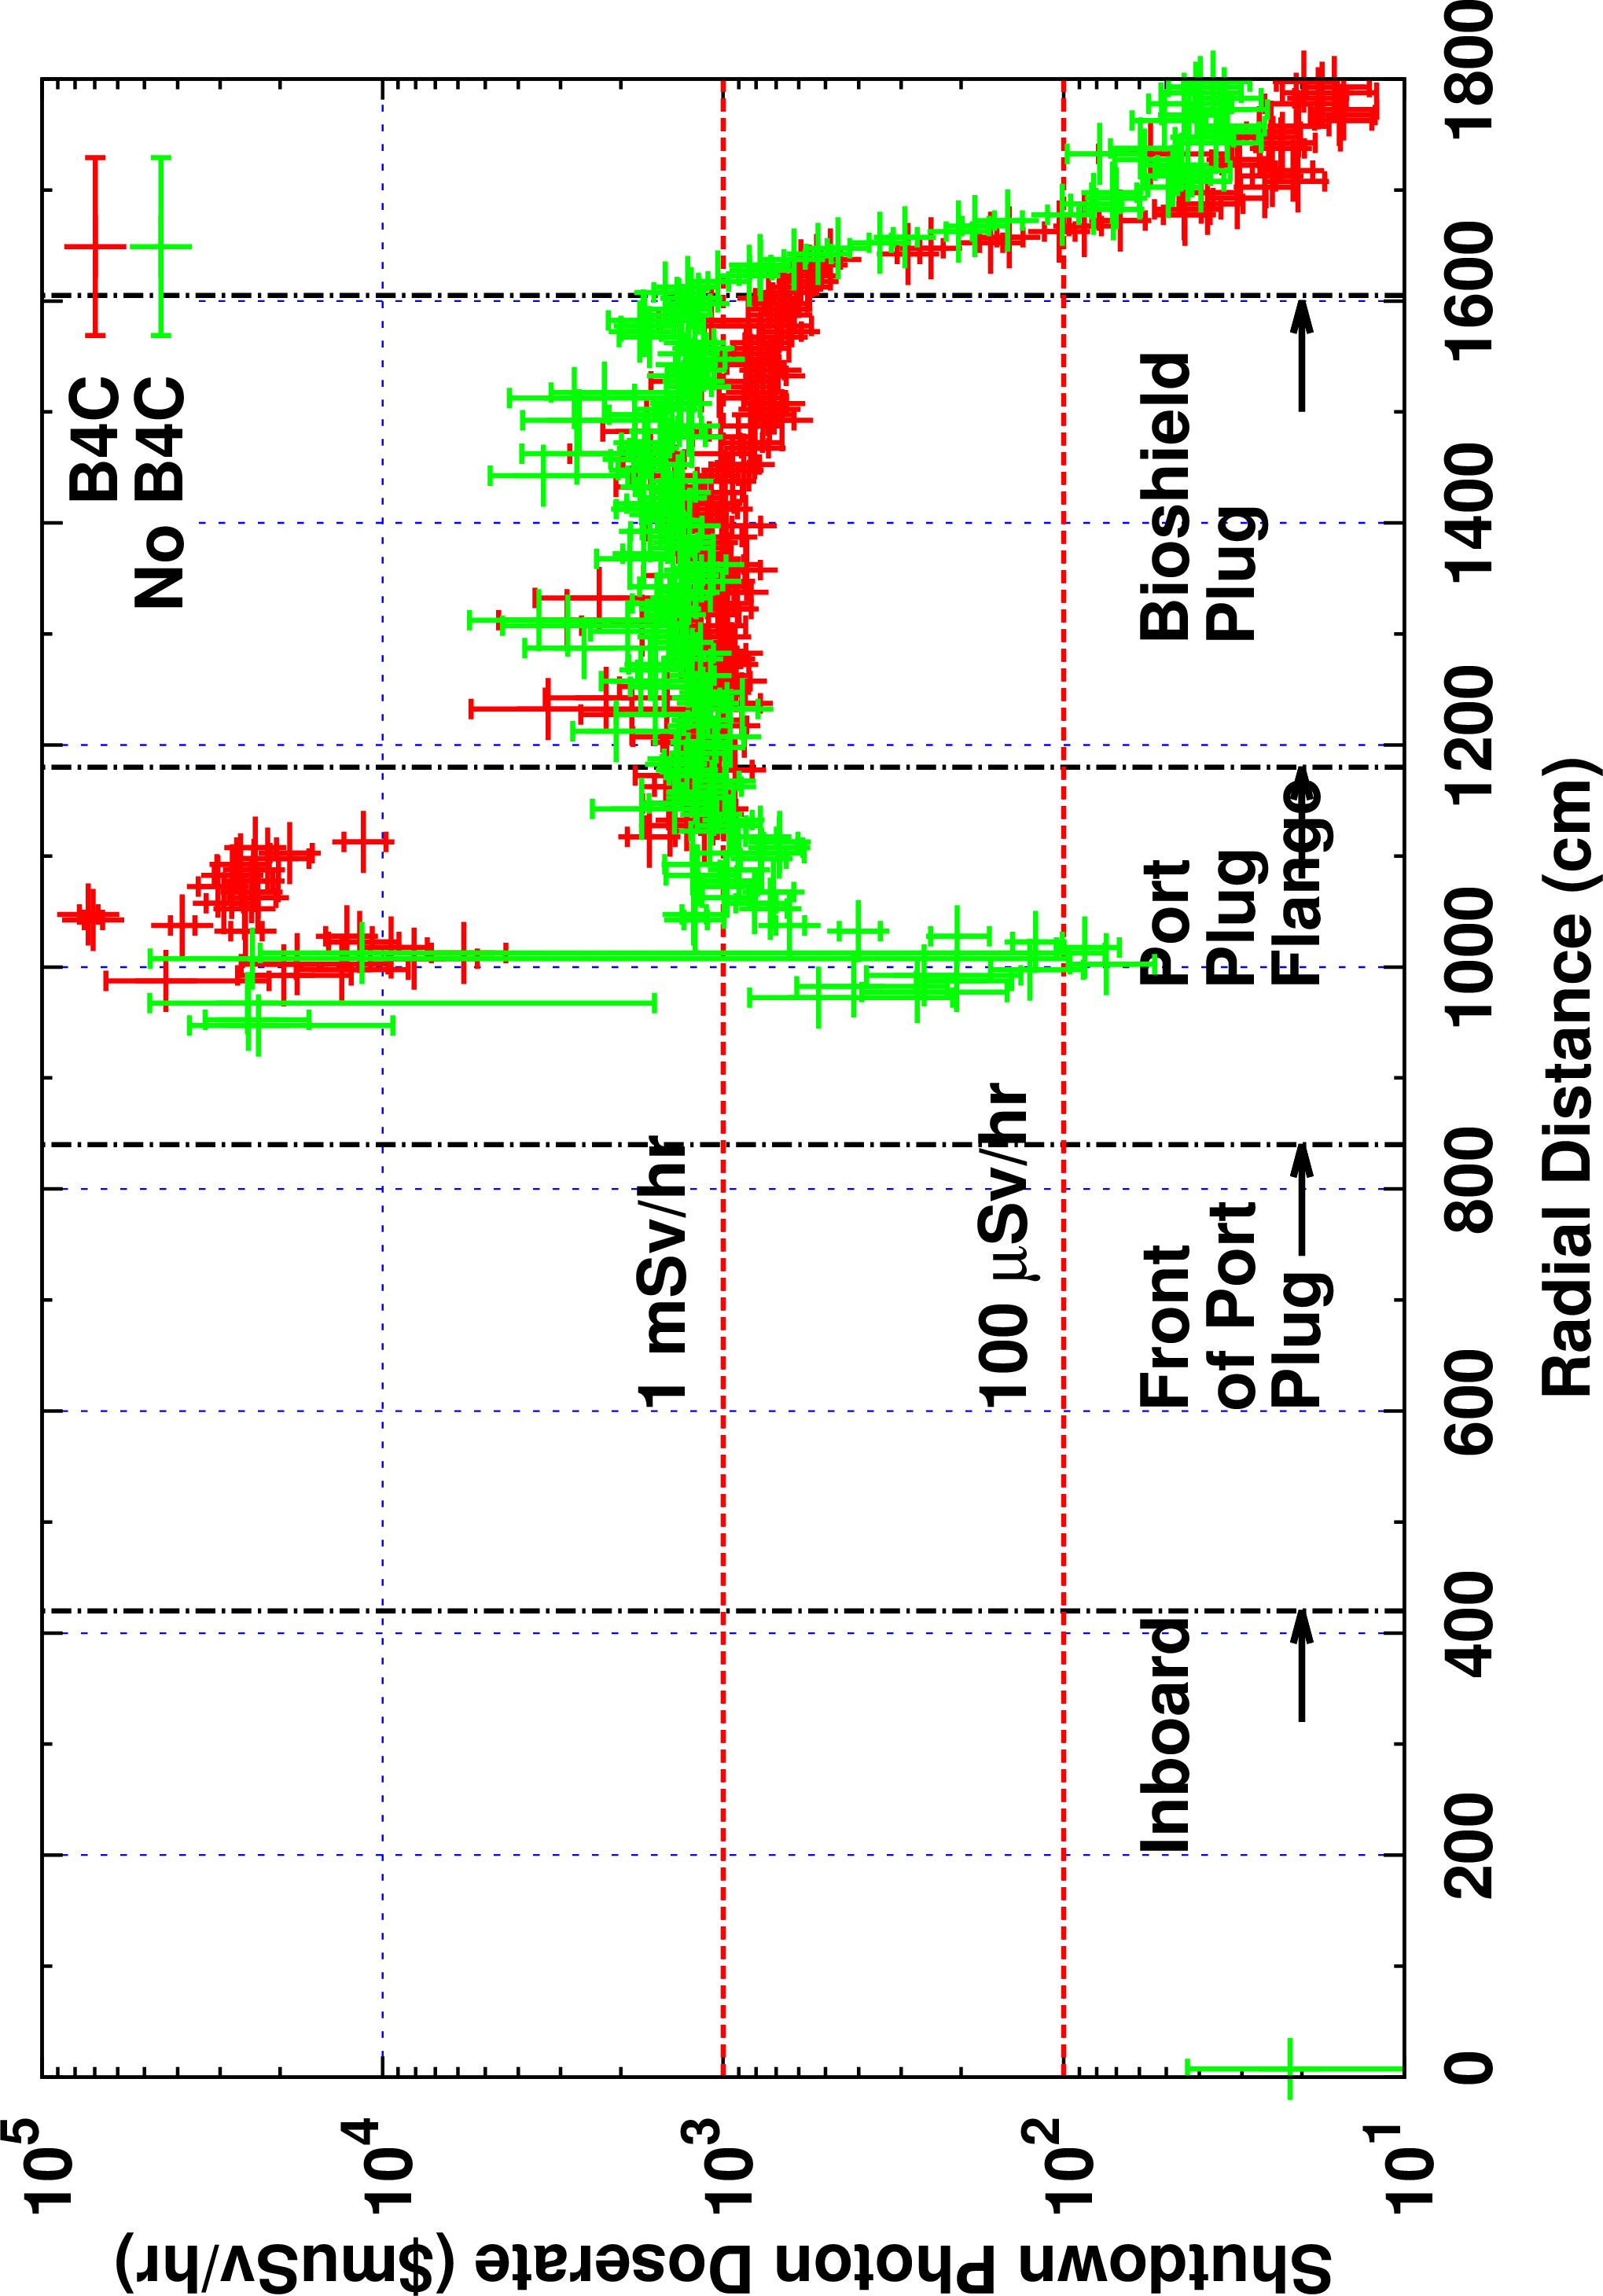
\includegraphics[clip,scale=0.12,angle=-90]{../plots/photon_lineout/comp/5yr_dc1.png}
\caption{Total dose rate along a line from 0,0,60 to 1800,0,60 cm for the 5 year irradiation
for both the B$_4$C and No B$_4$C case at $10^5$ s}
\label{fig:photons_5y_dc1_dose}
\end{figure}
\begin{figure}[ht!]
\centering
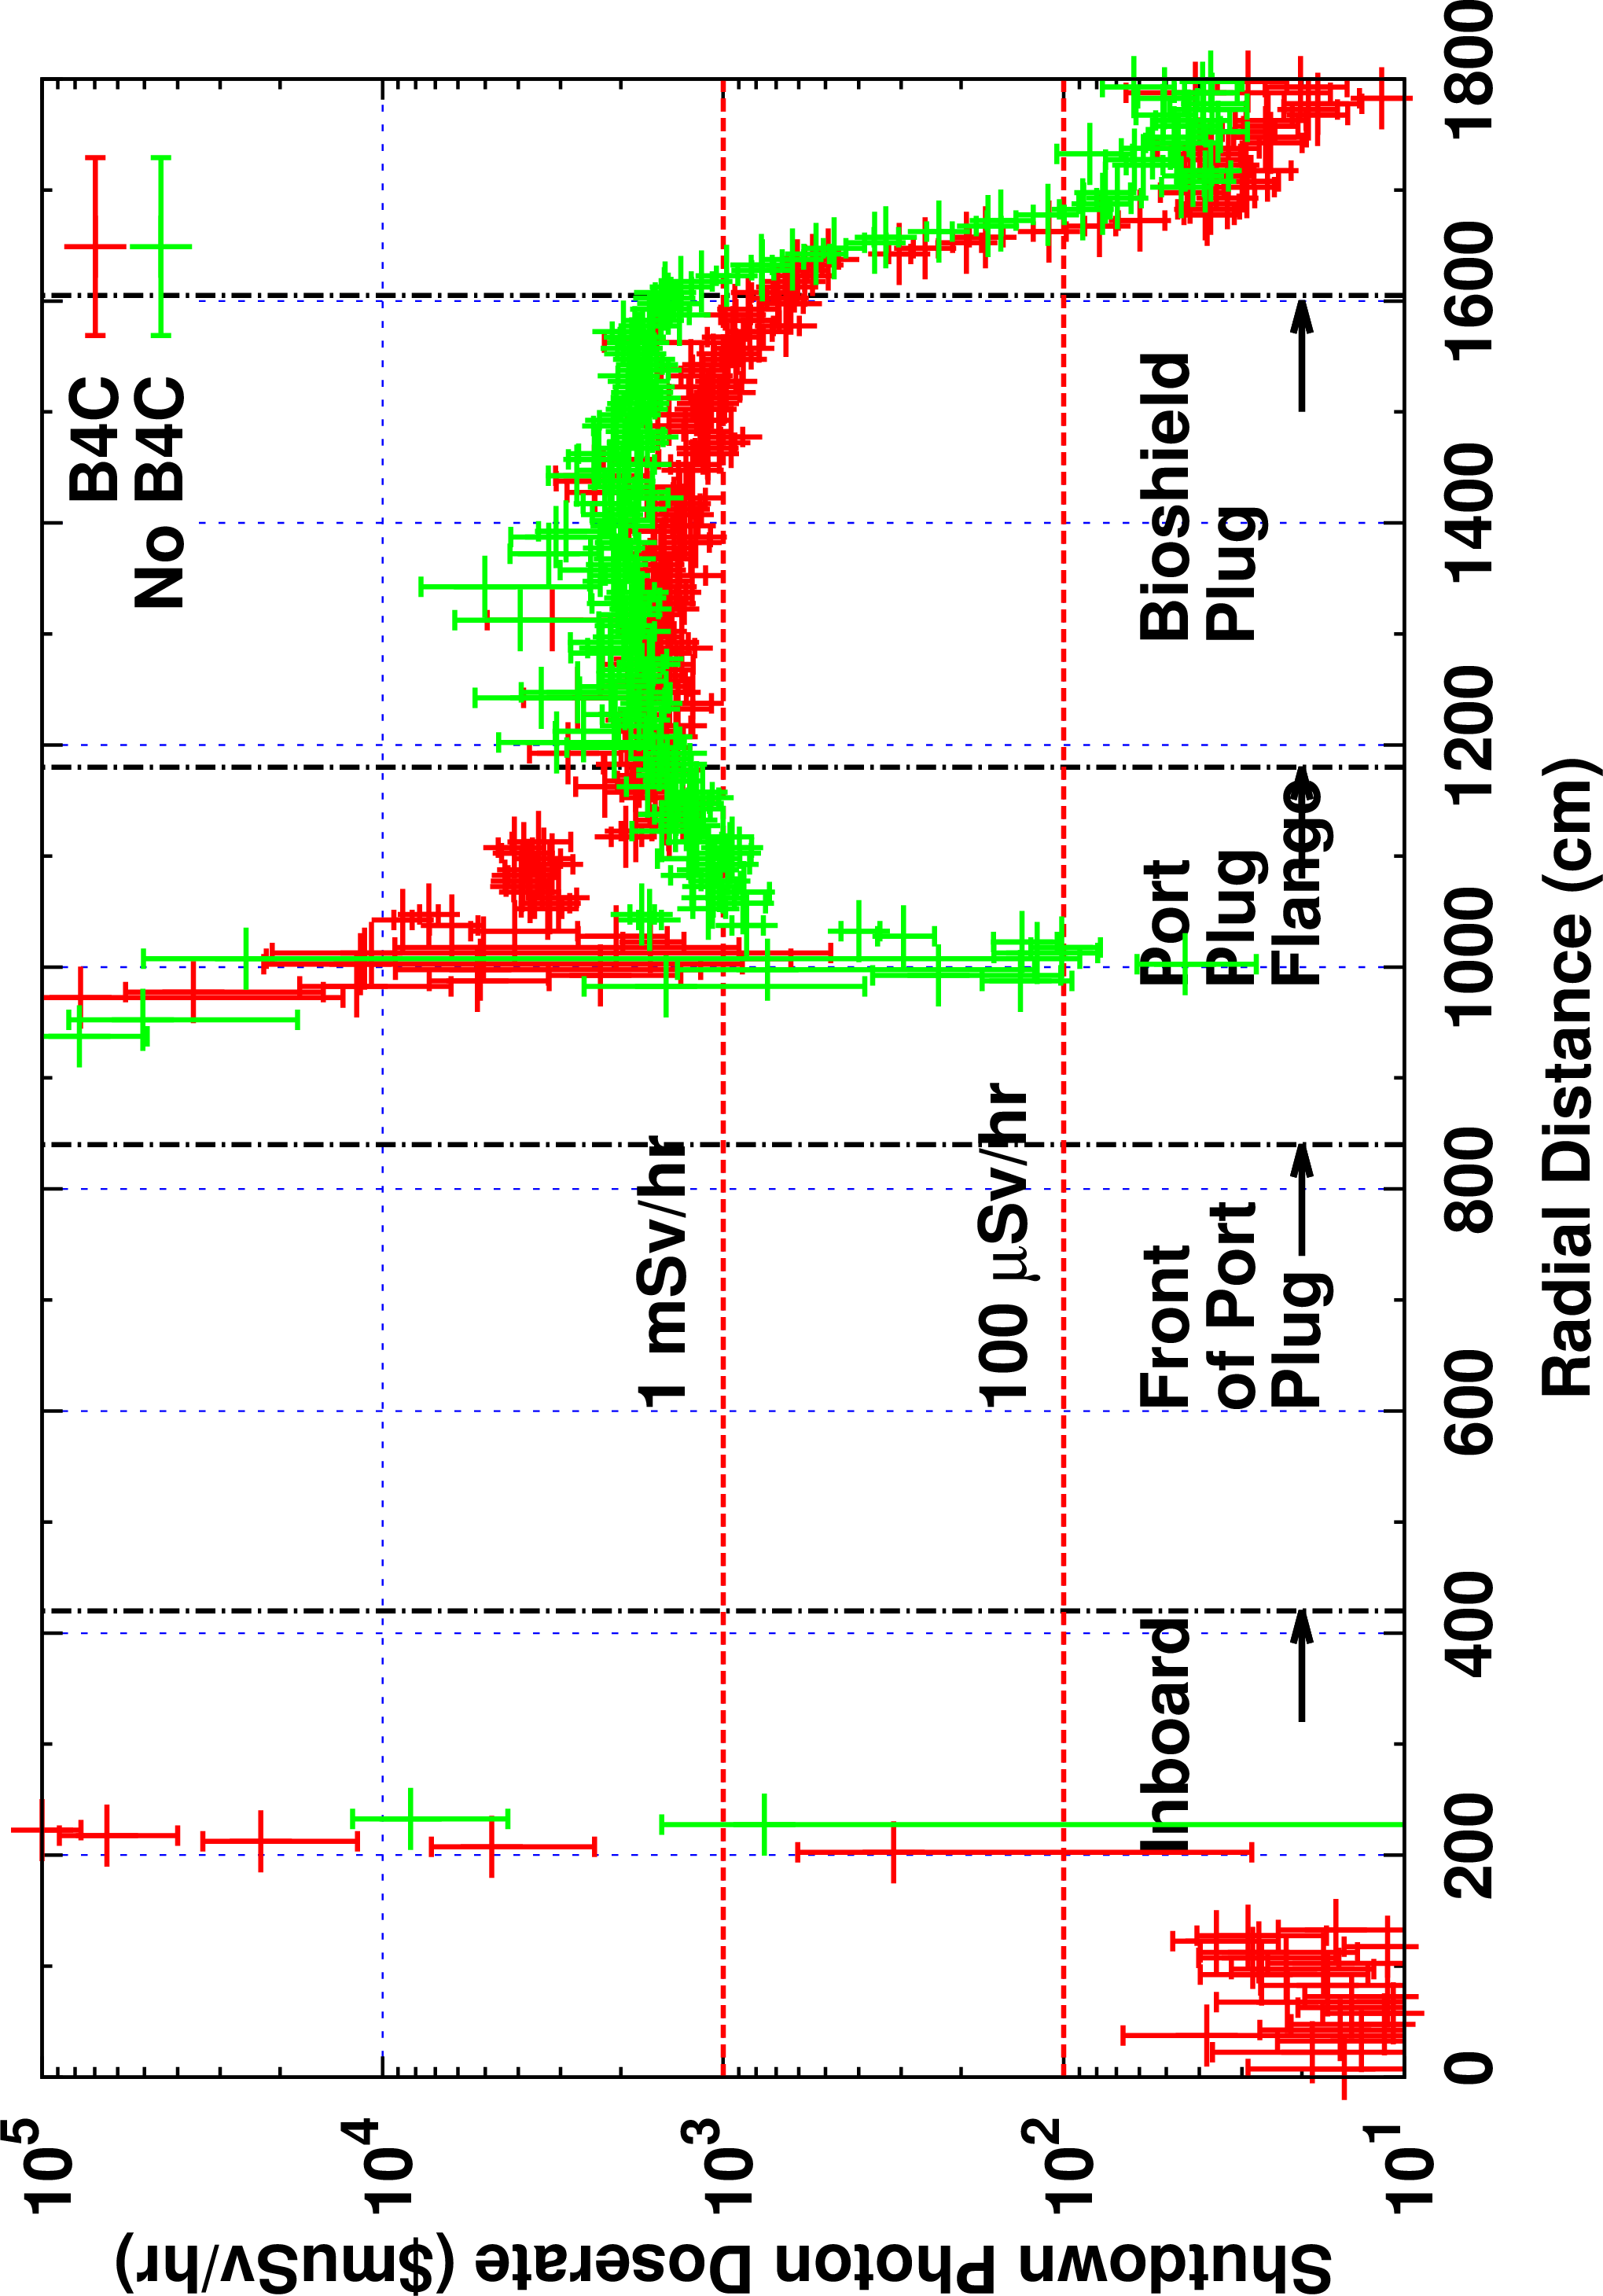
\includegraphics[clip,scale=0.12,angle=-90]{../plots/photon_lineout/comp/10yr_dc1.png}
\caption{Total dose rate along a line from 0,0,60 to 1800,0,60 cm for the 10 year irradiation
for both the B$_4$C and No B$_4$C case at $10^5$ s}
\label{fig:photons_10y_dc1_dose}
\end{figure}
\newpage
\subsubsection{Decay Time 2 - 1$\times$10$^{6}$ s}
\begin{figure}[ht!]
\centering
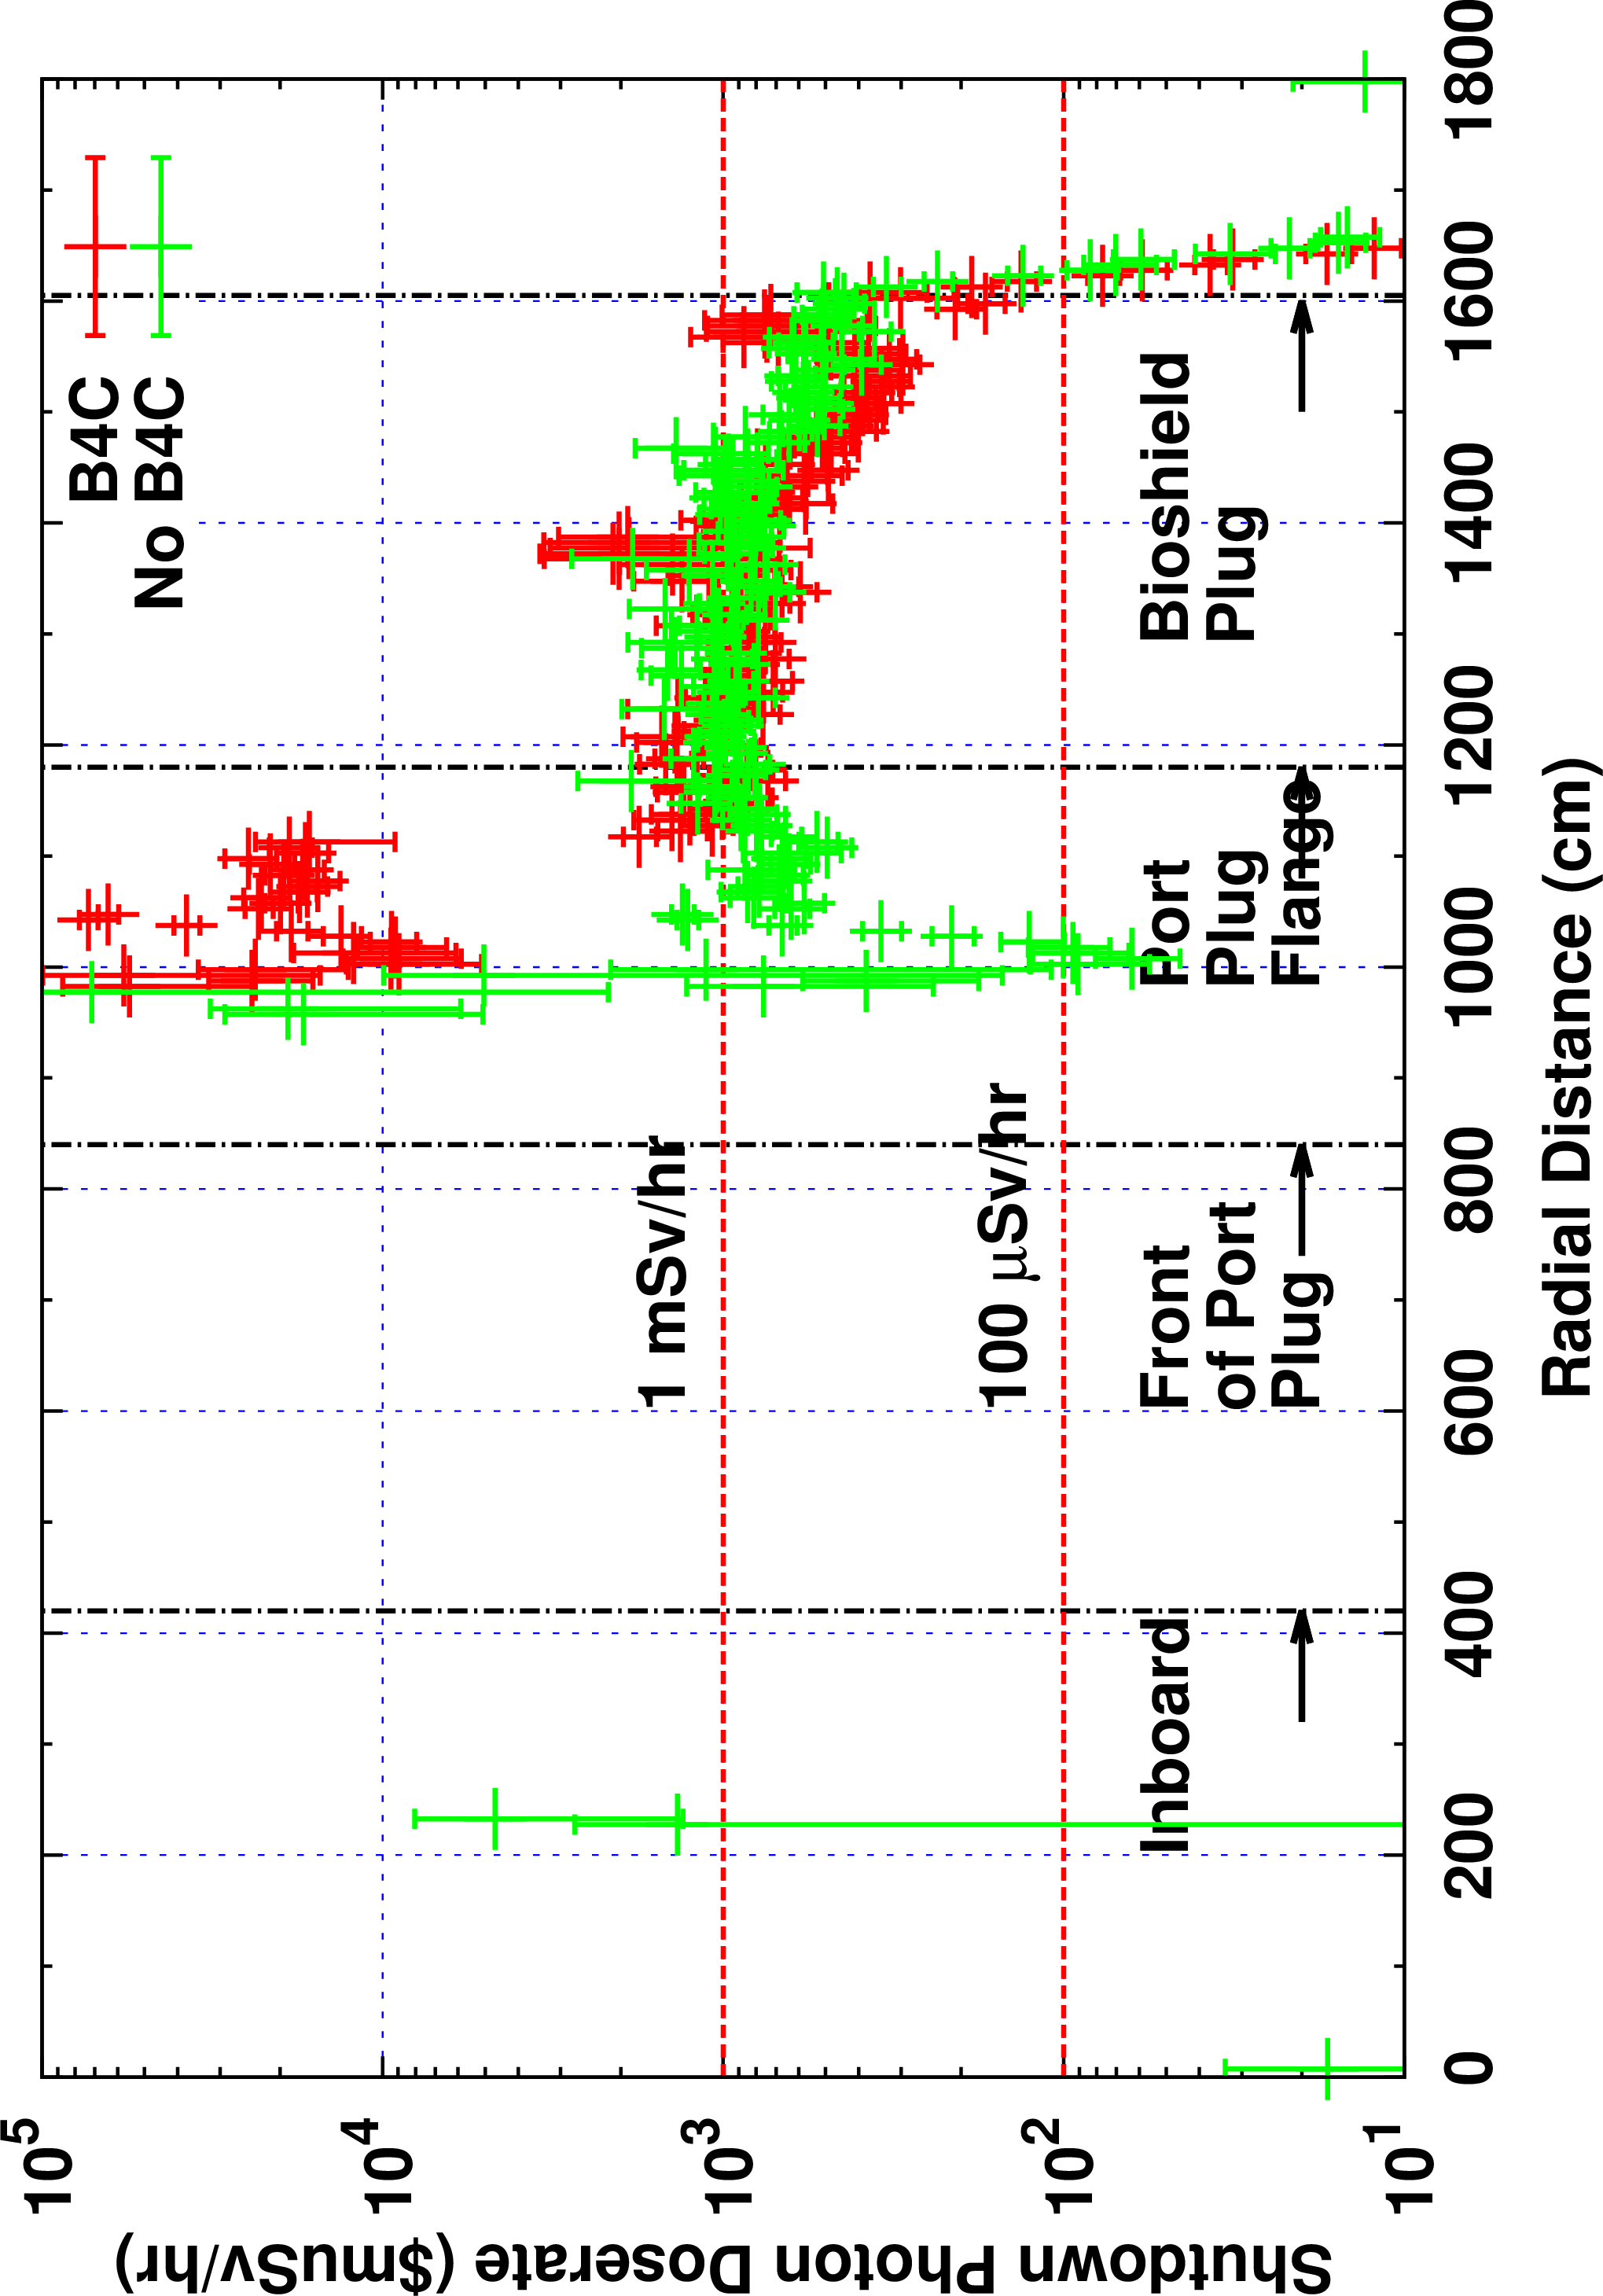
\includegraphics[clip,scale=0.12,angle=-90]{../plots/photon_lineout/comp/5yr_dc2.png}
\caption{Total dose rate along a line from 0,0,60 to 1800,0,60 cm for the 5 year irradiation
for both the B$_4$C and No B$_4$C case at $10^6$ s}
\label{fig:photons_5y_dc2_dose}
\end{figure}
\begin{figure}[ht!]
\centering
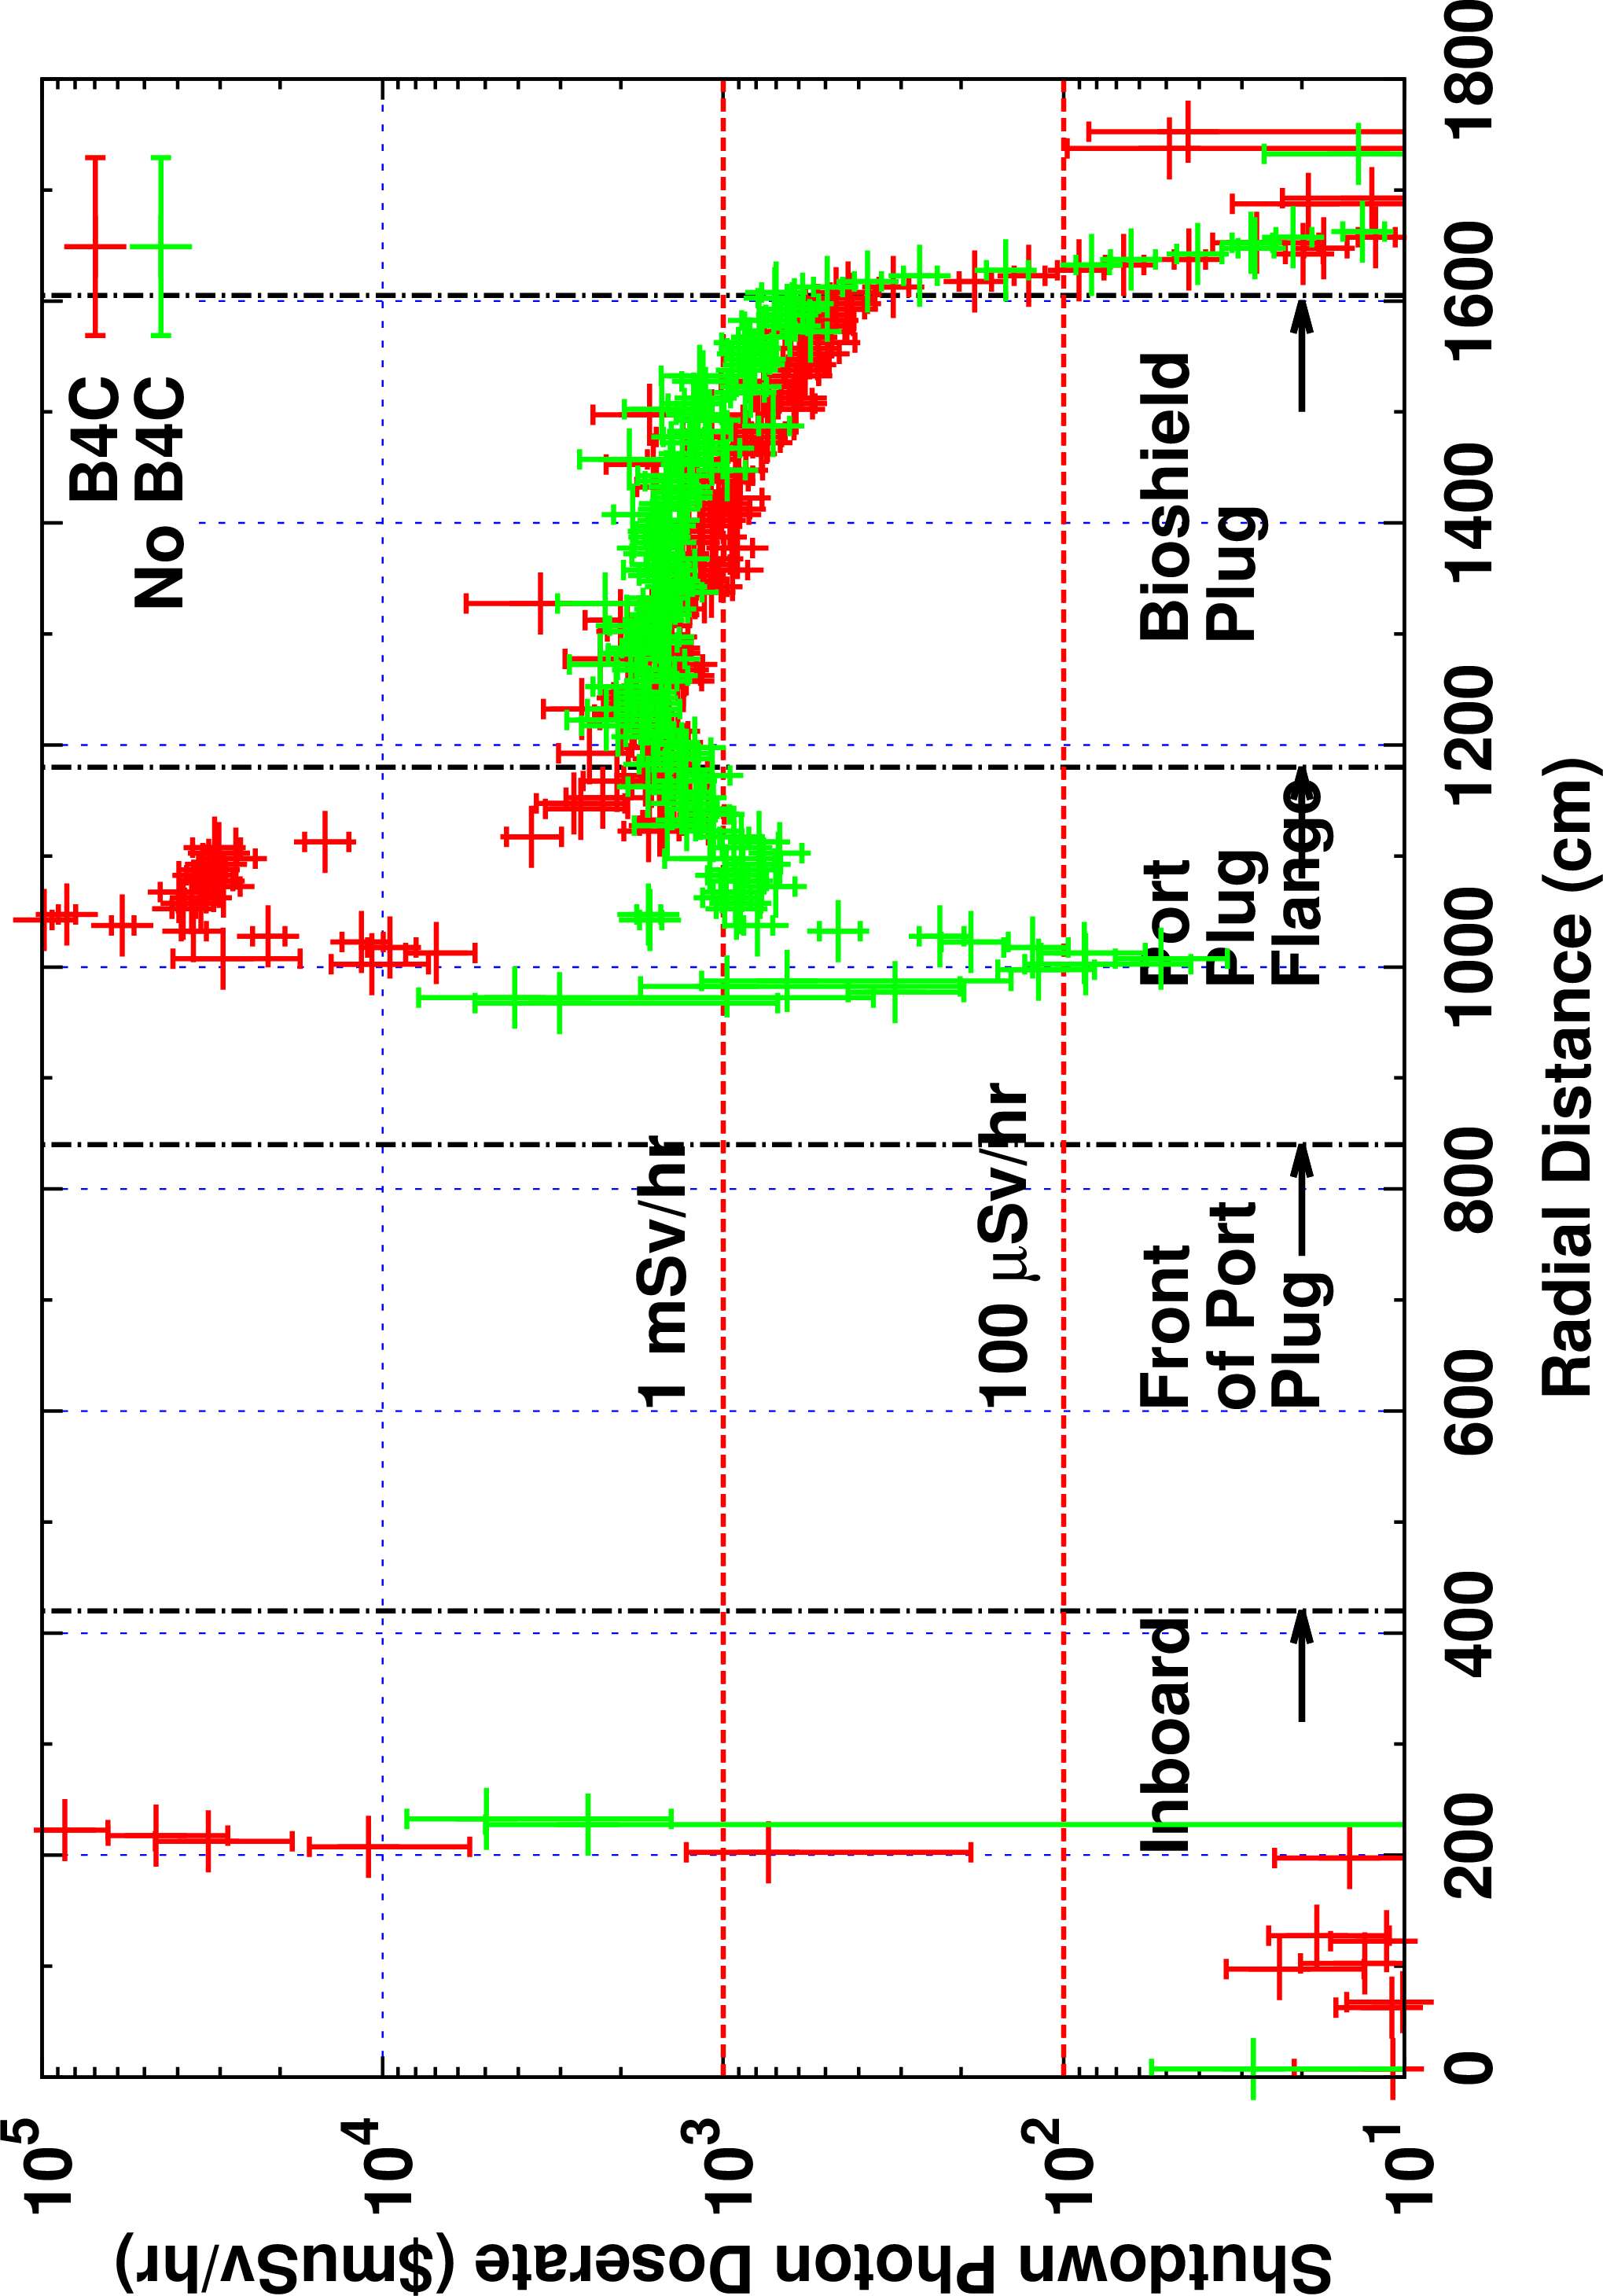
\includegraphics[clip,scale=0.12,angle=-90]{../plots/photon_lineout/comp/10yr_dc2.png}
\caption{Total dose rate along a line from 0,0,60 to 1800,0,60 cm for the 10 year irradiation
for both the B$_4$C and No B$_4$C case at $10^6$ s}
\label{fig:photons_10y_dc2_dose}
\end{figure}
\newpage
\subsubsection{Decay Time 3 - 1$\times$10$^{7}$ s}
\begin{figure}[ht!]
\centering
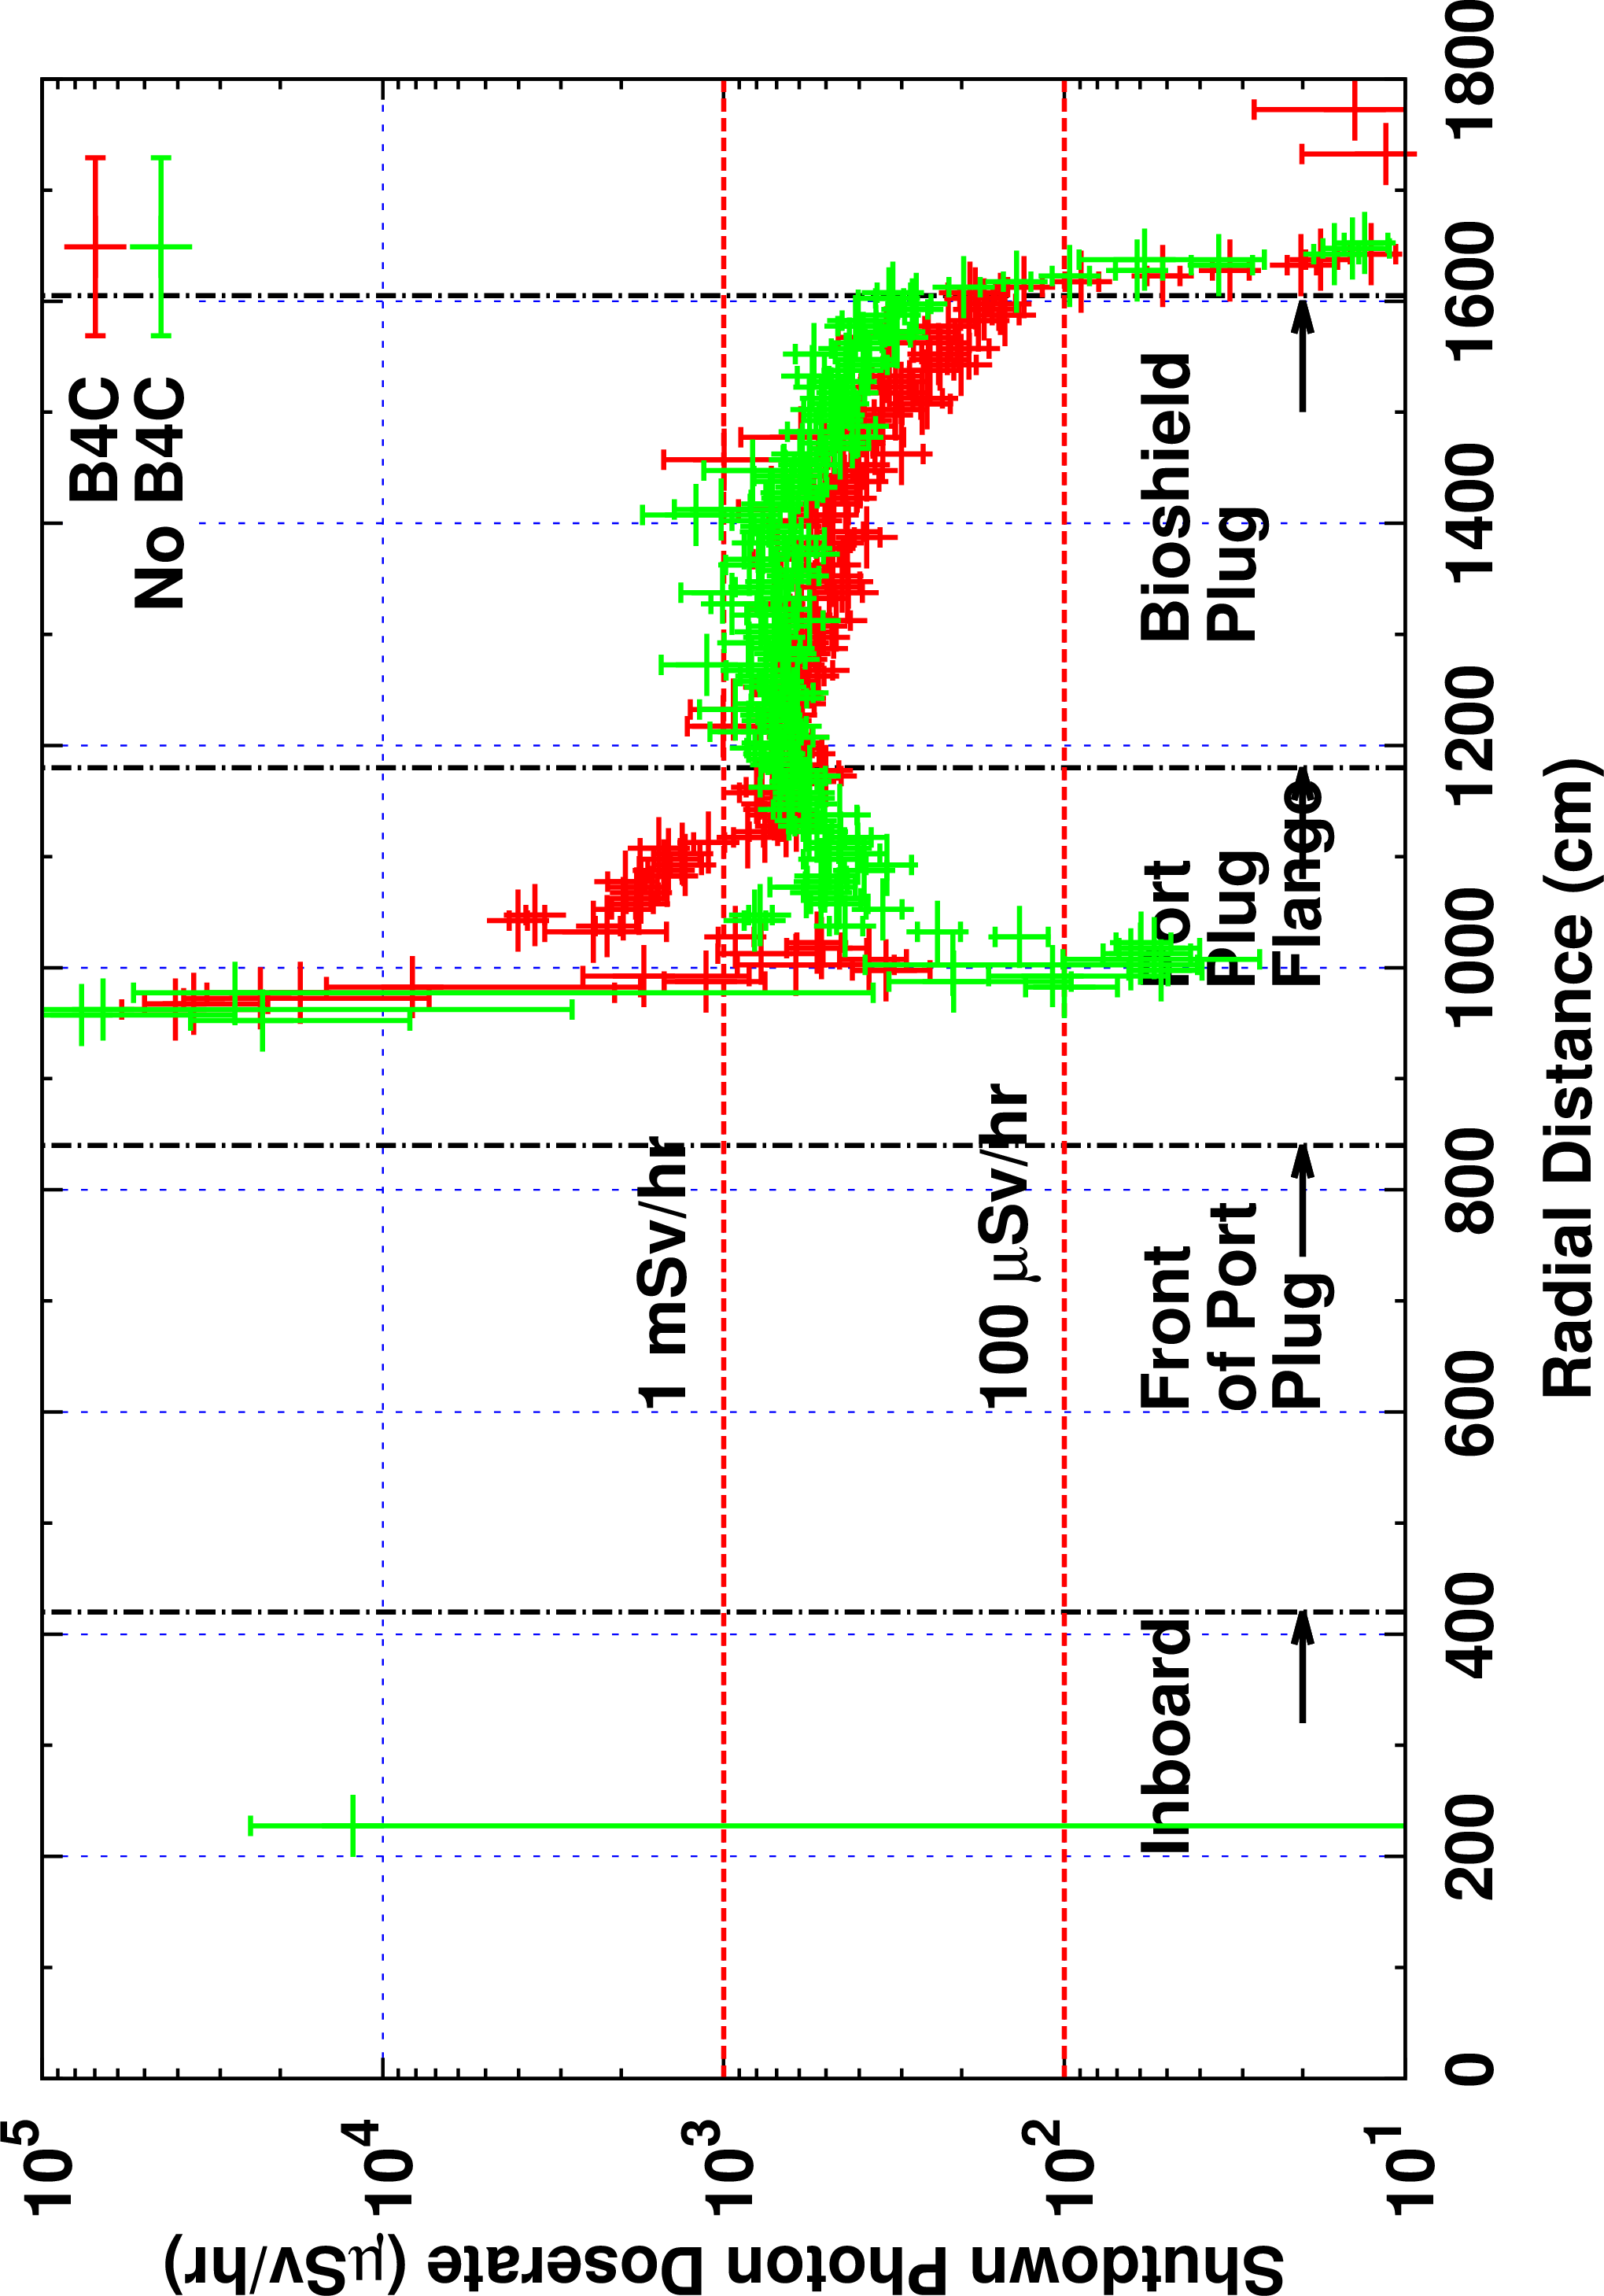
\includegraphics[clip,scale=0.12,angle=-90]{../plots/photon_lineout/comp/5yr_dc3.png}
\caption{Total dose rate along a line from 0,0,60 to 1800,0,60 cm for the 5 year irradiation
for both the B$_4$C and No B$_4$C case at $10^7$ s}
\label{fig:photons_5y_dc3_dose}
\end{figure}
\begin{figure}[ht!]
\centering
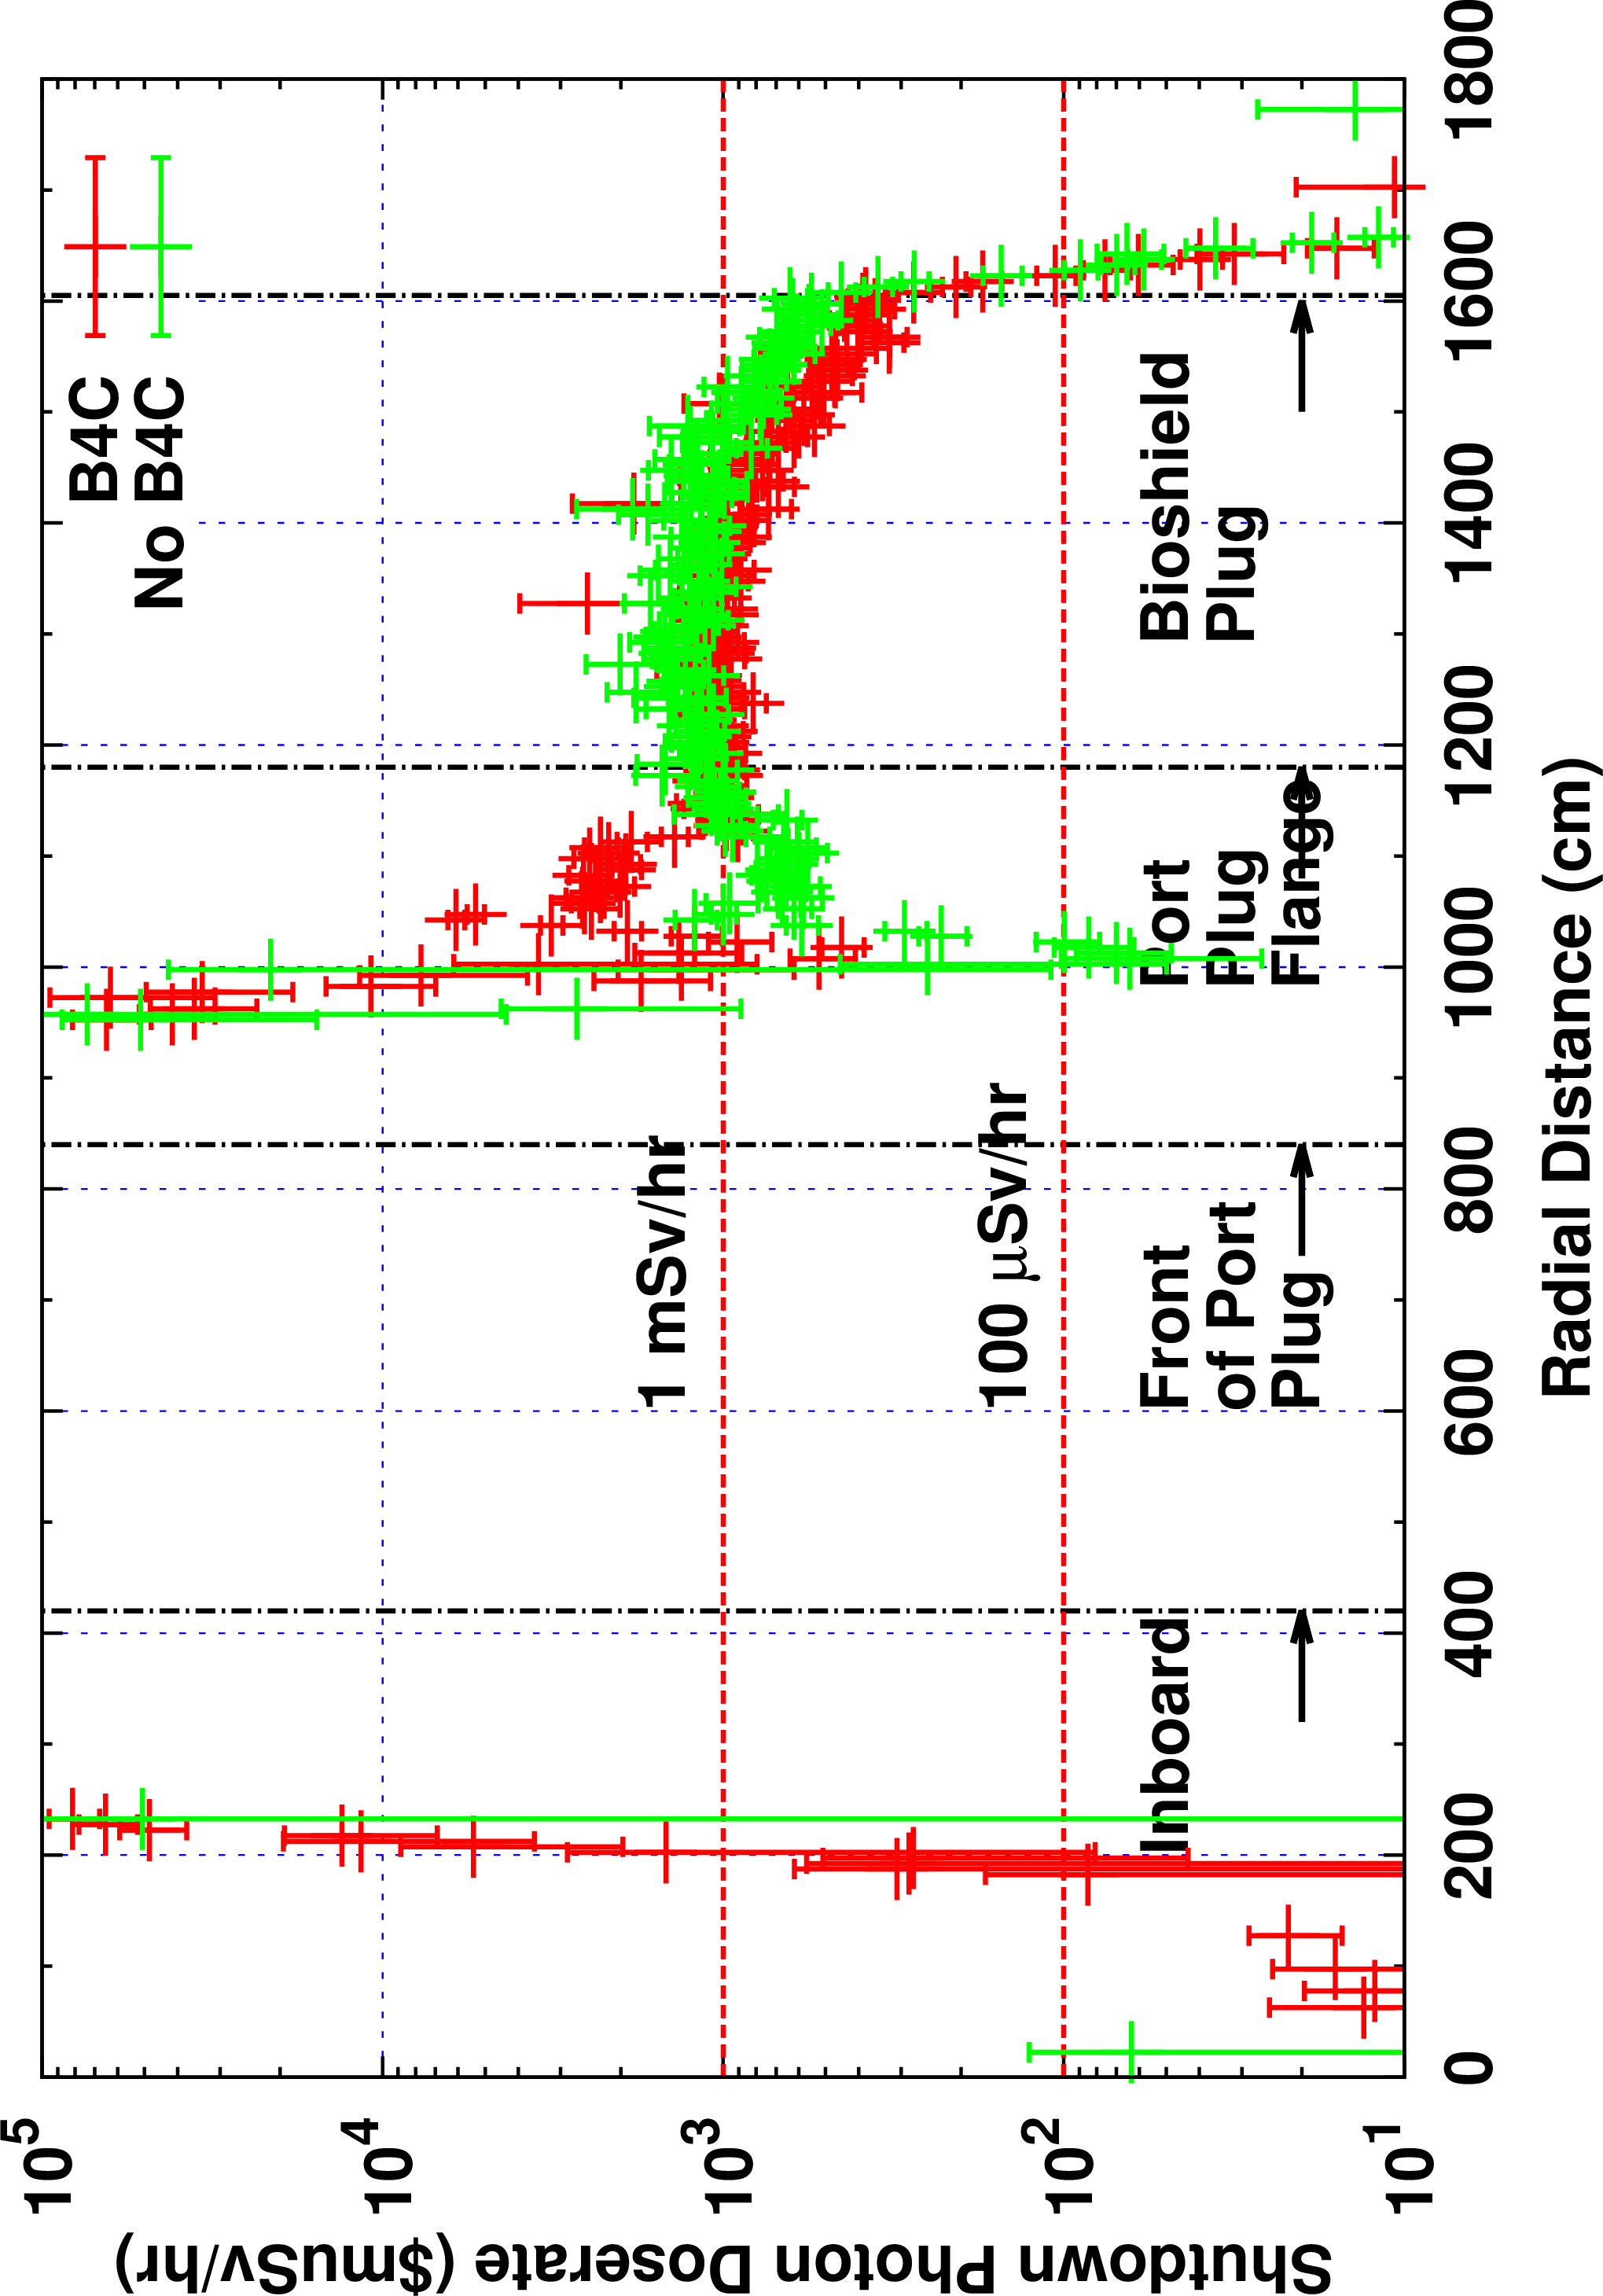
\includegraphics[clip,scale=0.12,angle=-90]{../plots/photon_lineout/comp/10yr_dc3.png}
\caption{Total dose rate along a line from 0,0,60 to 1800,0,60 cm for the 10 year irradiation
for both the B$_4$C and No B$_4$C case at $10^7$ s}
\label{fig:photons_10y_dc3_dose}
\end{figure}
\clearpage
\newpage
\subsection{Summary}
\subsubsection*{B$_4$C}
There are difference between the two irradiations across the decay times, 
the 5 year irradiation case values are $\sim$ 0.75 times that of the 10 year 
case, which is itself $\sim$ 0.75 times that of the full SA-2 scenario. Of note
is that most points within equatorial port interspace are below 1 mSv/hr.
\subsubsection*{No B$_4$C}
Similarly to the B$_4$C case, thhere are difference between the two irradiations
across the decay times, the 5 year irradiation case values are $\sim$ 0.75 times
 that of the 10 year case, which is itself $\sim$ 0.75 times that of the full 
SA-2 scenario. Of note is that for the 10 year irradiation and for all decay 
times most points in the equatorial port interspace is above 1 mSv/hr. However,
for the 5 year irradiation we see that by the second decay time most points 
are under 1 mSv/hr. 
\subsubsection*{Comparison}
The immediate differences between the B$_4$C and no B$_4$C are the same as in 
the full report, in the port interspace the SDR is lower adjacent to the 
bioshield for all cases across all decay times. There are some cases where
just behind the equatorial port plug flange the dose can be higher in the 
B$_4$C than in the no B$_4$C case, this is likley due to a large error in the 
activation source there due to a poor estimate of the neutron flux. 
\clearpage
\newpage
\section{Conclusion}
A set of sequence of neutron activation calculations were peformed for a suite 
of 3 different irradiation scenarios. It was found that lower the 5 and 10 year
irradiation times reduce the SDR by factors of 0.56 relative to the SA2 and
0.75 relative to the SA2 scenario respectively.

\begin{table}[ht!]
   \centering      
   \begin{tabular}{| c | c | c | c |}
      \hline
      & SA2 & 10 Yr & 5 Yr \\
      \hline
      Decay Time (s) & Dose Rate & Dose Rate & Dose Rate \\
      \hline
      1.0$\times$10$^{5}$ & 1.257$\times$10$^{3}$ & 7.700$\times$10$^{2}$ & 6.624$\times$10$^{2}$ \\
      1.0$\times$10$^{6}$ & 4.543$\times$10$^{2}$ & 4.295$\times$10$^{2}$ & 3.706$\times$10$^{2}$ \\
      1.0$\times$10$^{7}$ & 3.761$\times$10$^{2}$ & 2.756$\times$10$^{2}$ & 1.895$\times$10$^{2}$ \\
      \hline
\end{tabular}
\caption{B4C Results}
\label{tab:b4c_summary_scenario}
\end{table}

\begin{table}[ht!]
   \centering      
   \begin{tabular}{| c | c | c | c |}
      \hline
      & SA2 & 10 Yr & 5 Yr \\
      \hline
      Decay Time (s) & Dose Rate & Dose Rate & Dose Rate \\
      \hline
      1.0$\times$10$^{5}$ & 2.426$\times$10$^{3}$ & 1.481$\times$10$^{3}$ & 1.478$\times$10$^{3}$ \\
      1.0$\times$10$^{6}$ & 1.936$\times$10$^{3}$ & 1.481$\times$10$^{3}$ & 1.936$\times$10$^{2}$ \\
      1.0$\times$10$^{7}$ & 6.750$\times$10$^{2}$ & 4.501$\times$10$^{2}$ & 6.750$\times$10$^{2}$ \\
      \hline
\end{tabular}
\caption{No B4C Results}
\label{tab:nob4c_summary_scenario}
\end{table}

The SDR results for the shortened irradiation times show the expected behavior 
that shorter irradiation times lead to lower accumulated activities and therfore
lower SDR.  


\newpage
\bibliographystyle{unsrt}
\bibliography{bibliography}
\newpage
\clearpage
\section{Appendix A - B4C 5 Year Irradiation}
\begin{figure}[ht!]
\centering
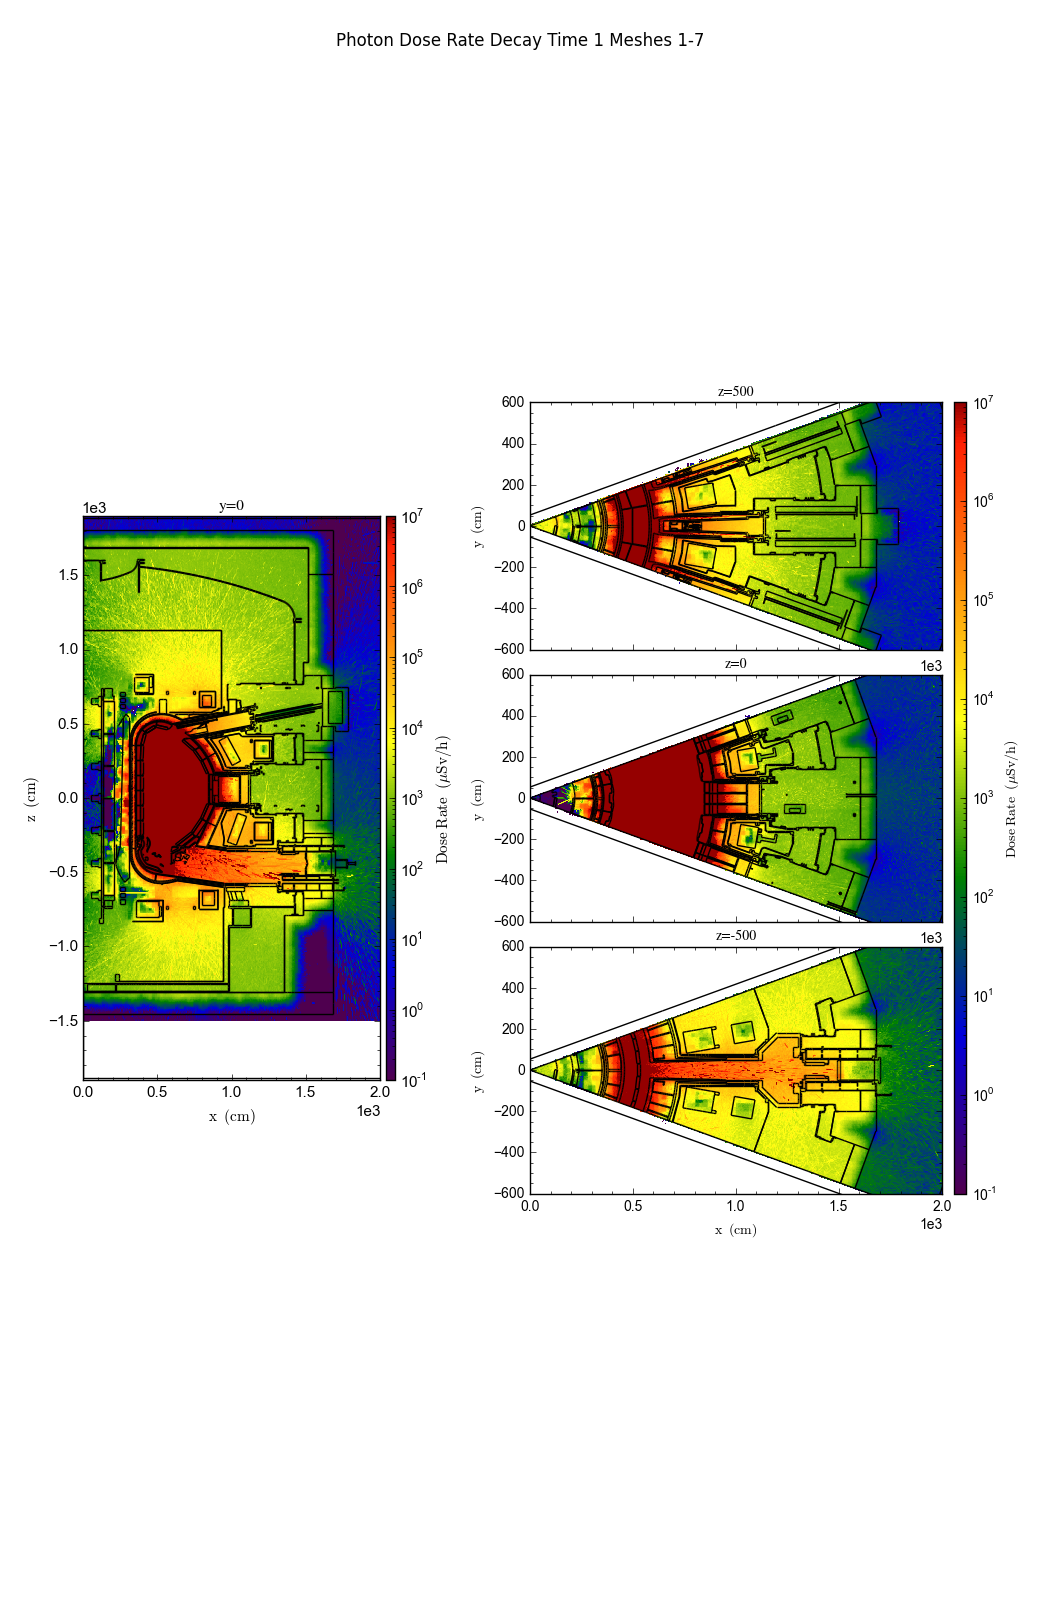
\includegraphics[trim={0cm 8cm, 0cm 8cm},clip,scale=0.75]{../plots/final_model_with_b4c/5year/Photon_Dose_Rate_Decay_Time_1_Meshes_1-7.png}
\caption{Total dose rate for decay time 1 for the 5 year irradiation}
\label{fig:photons_5y_dc1_nob4c_dose}
\end{figure}
\begin{figure}[ht!]
\centering
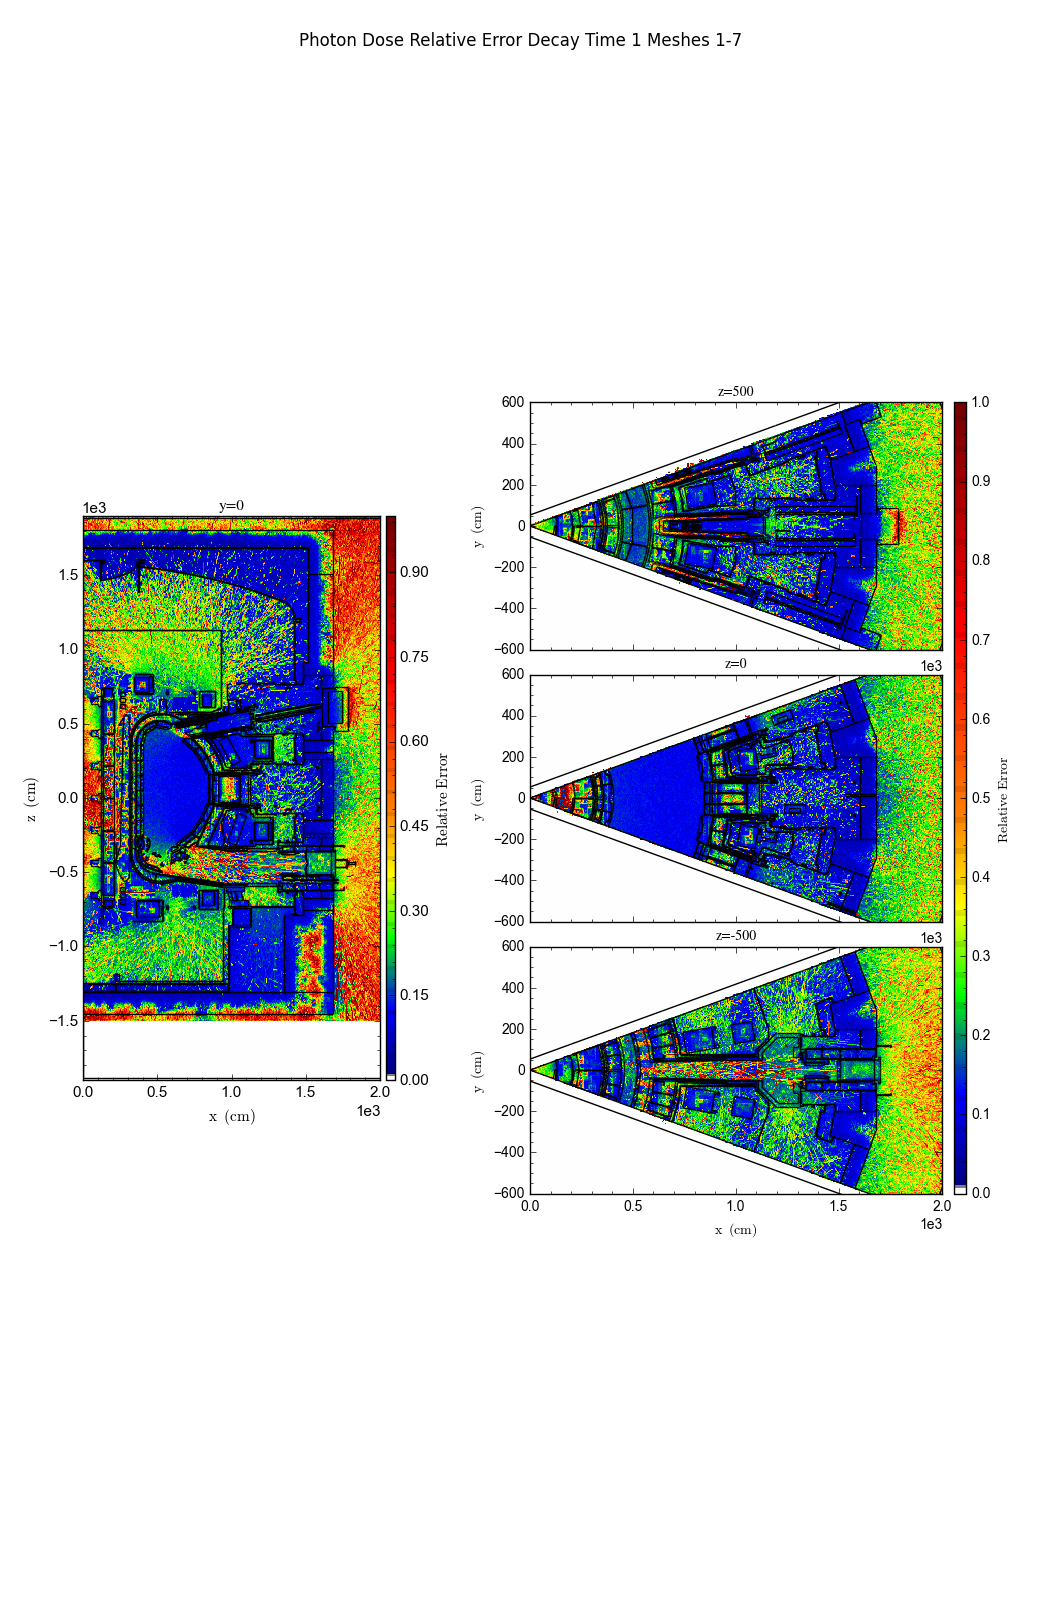
\includegraphics[trim={0cm 8cm, 0cm 8cm},clip,scale=0.75]{../plots/final_model_with_b4c/5year/Photon_Dose_Relative_Error_Decay_Time_1_Meshes_1-7.png}
\caption{Total dose rate relative error for decay time 1 for the 5 year irradiation}
\label{fig:photons_5y_dc1_nob4c_relerr}
\end{figure}
\clearpage
\begin{figure}[ht!]
\centering
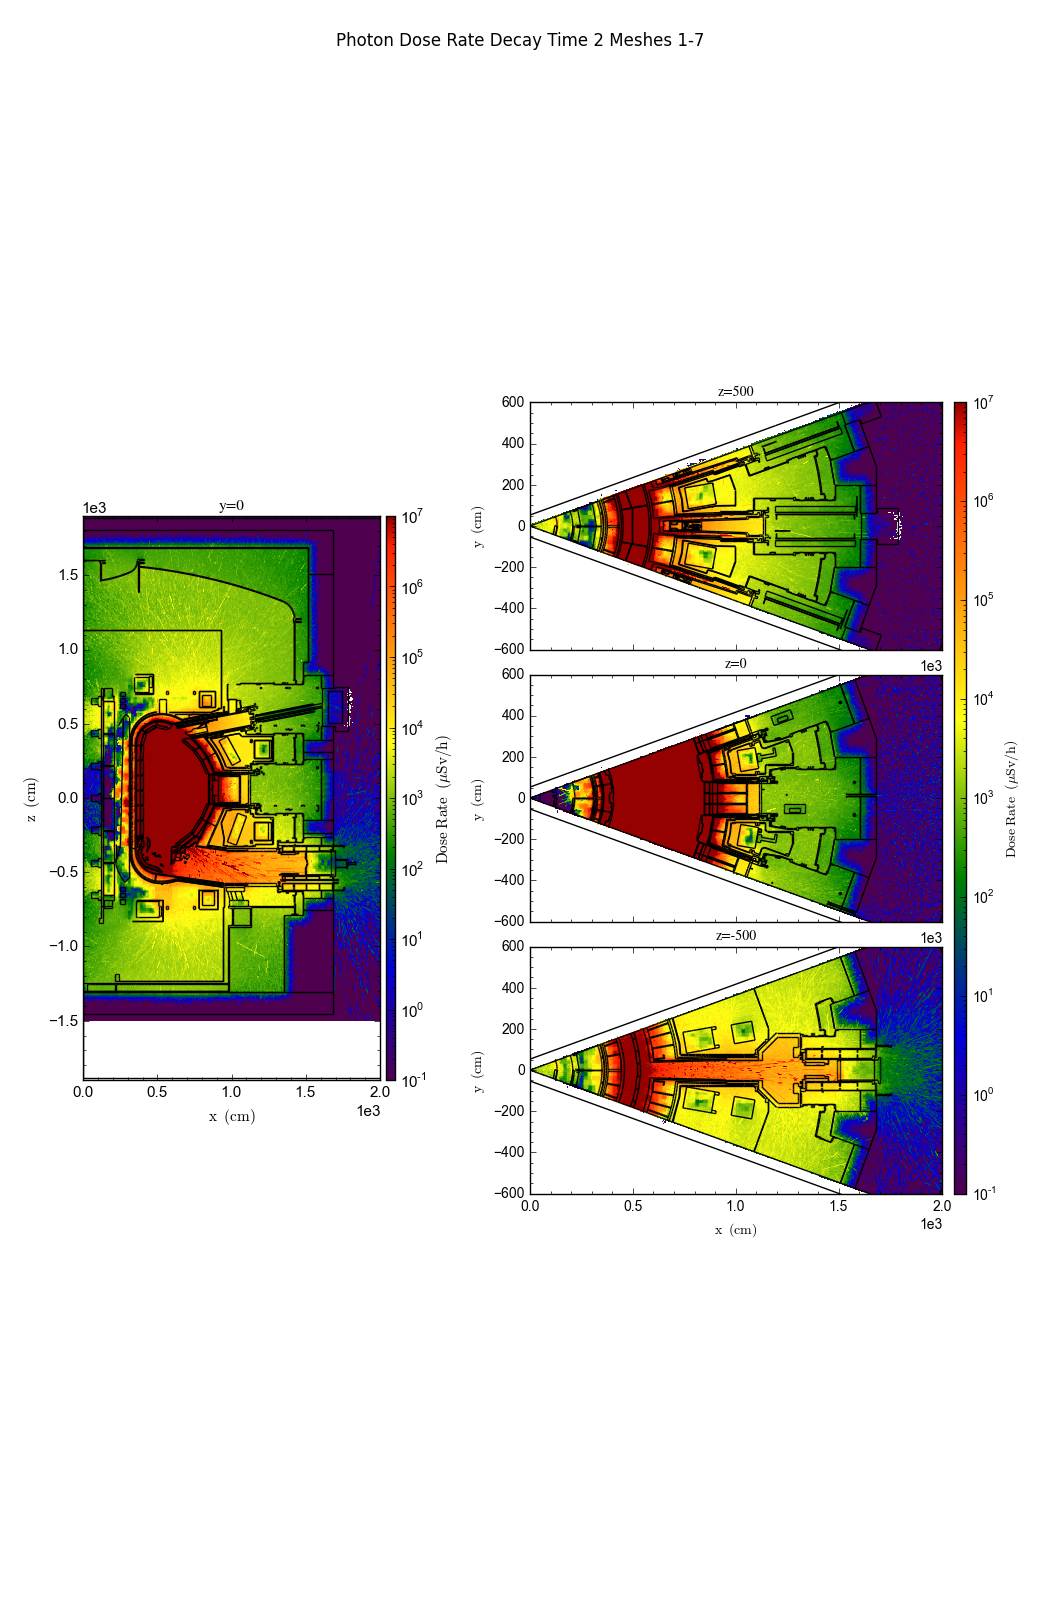
\includegraphics[trim={0cm 8cm, 0cm 8cm},clip,scale=0.75]{../plots/final_model_with_b4c/5year/Photon_Dose_Rate_Decay_Time_2_Meshes_1-7.png}
\caption{Total dose rate for decay time 2 for the 5 year irradiation}
\label{fig:photons_5y_dc2_nob4c_dose}
\end{figure}
\begin{figure}[ht!]
\centering
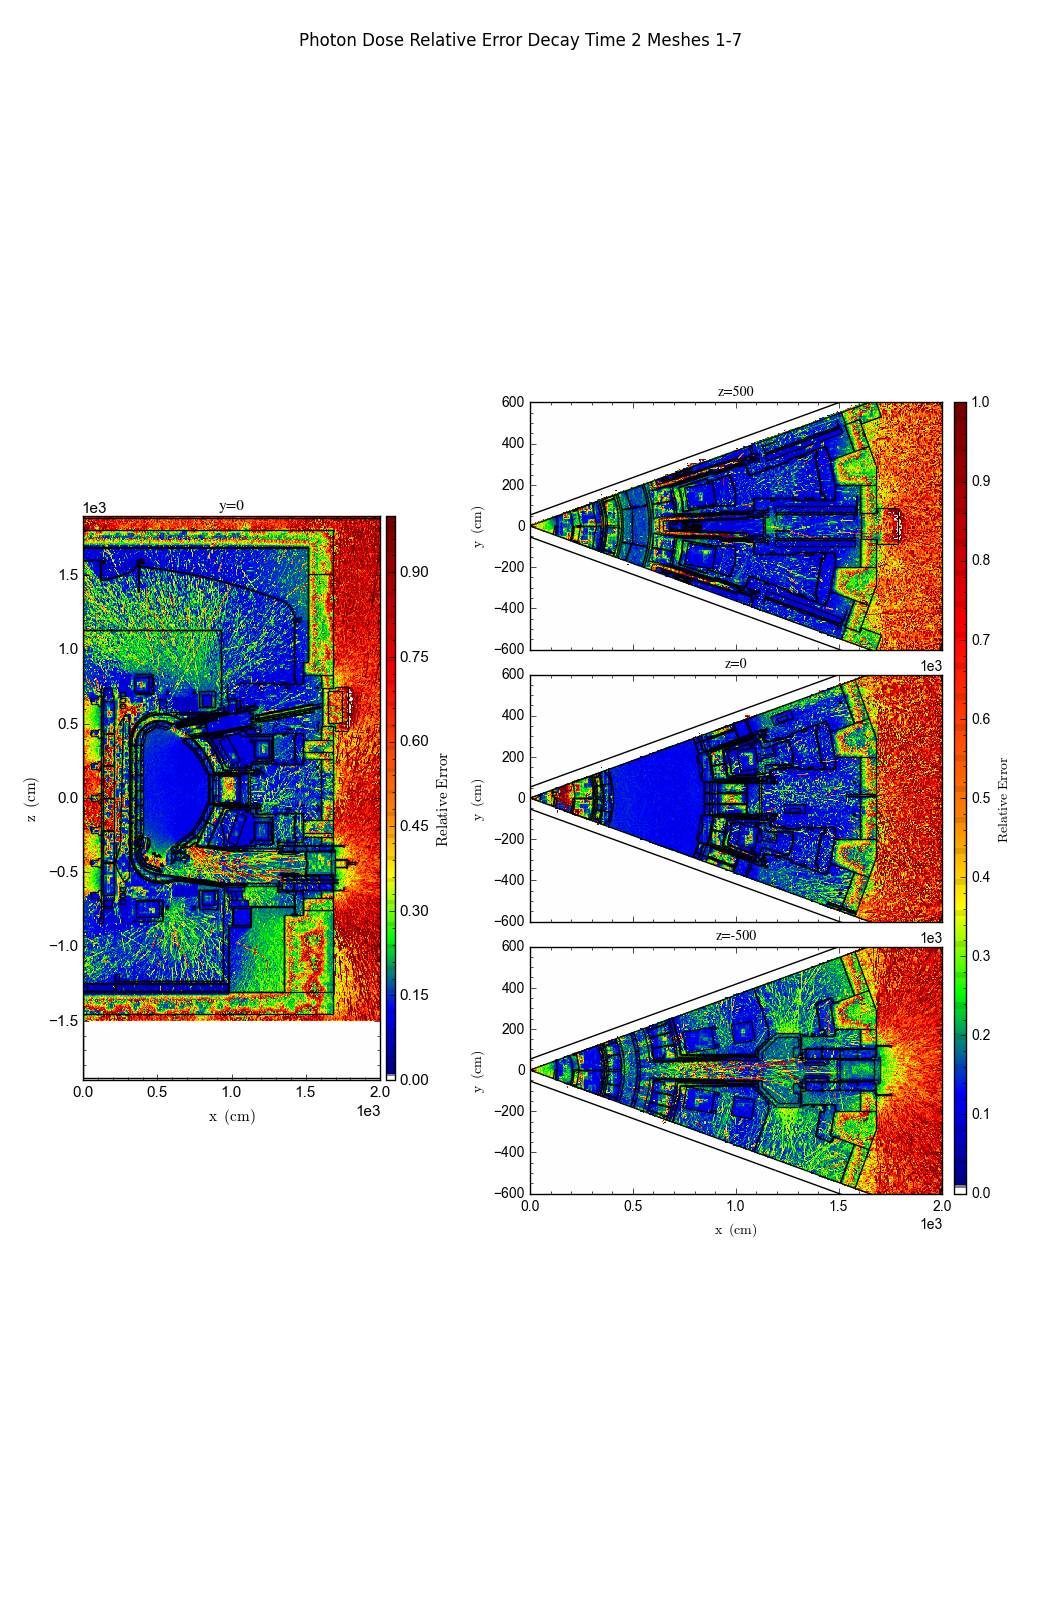
\includegraphics[trim={0cm 8cm, 0cm 8cm},clip,scale=0.75]{../plots/final_model_with_b4c/5year/Photon_Dose_Relative_Error_Decay_Time_2_Meshes_1-7.png}
\caption{Total dose rate relative error for decay time 2 for the 5 year irradiation}
\label{fig:photons_5y_dc2_nob4c_relerr}
\end{figure}
\clearpage
\begin{figure}[ht!]
\centering
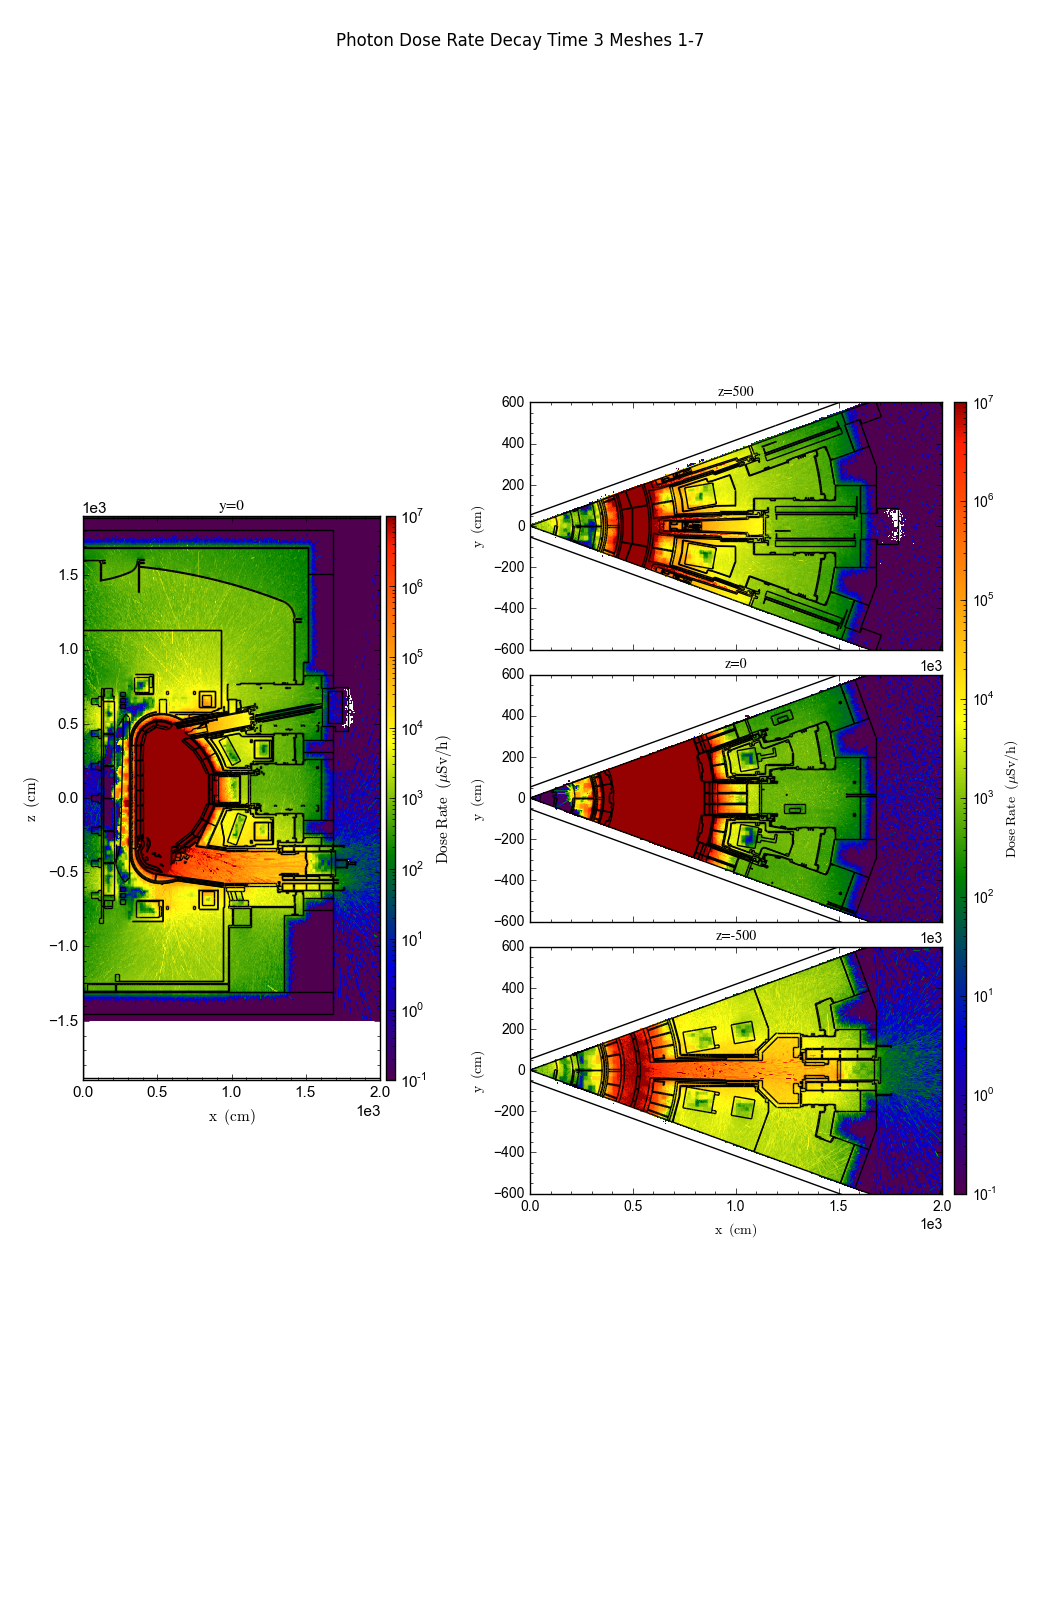
\includegraphics[trim={0cm 8cm, 0cm 8cm},clip,scale=0.75]{../plots/final_model_with_b4c/5year/Photon_Dose_Rate_Decay_Time_3_Meshes_1-7.png}
\caption{Total dose rate for decay time 3 for the 5 year irradiation}
\label{fig:photons_5y_dc3_nob4c_dose}
\end{figure}
\begin{figure}[ht!]
\centering
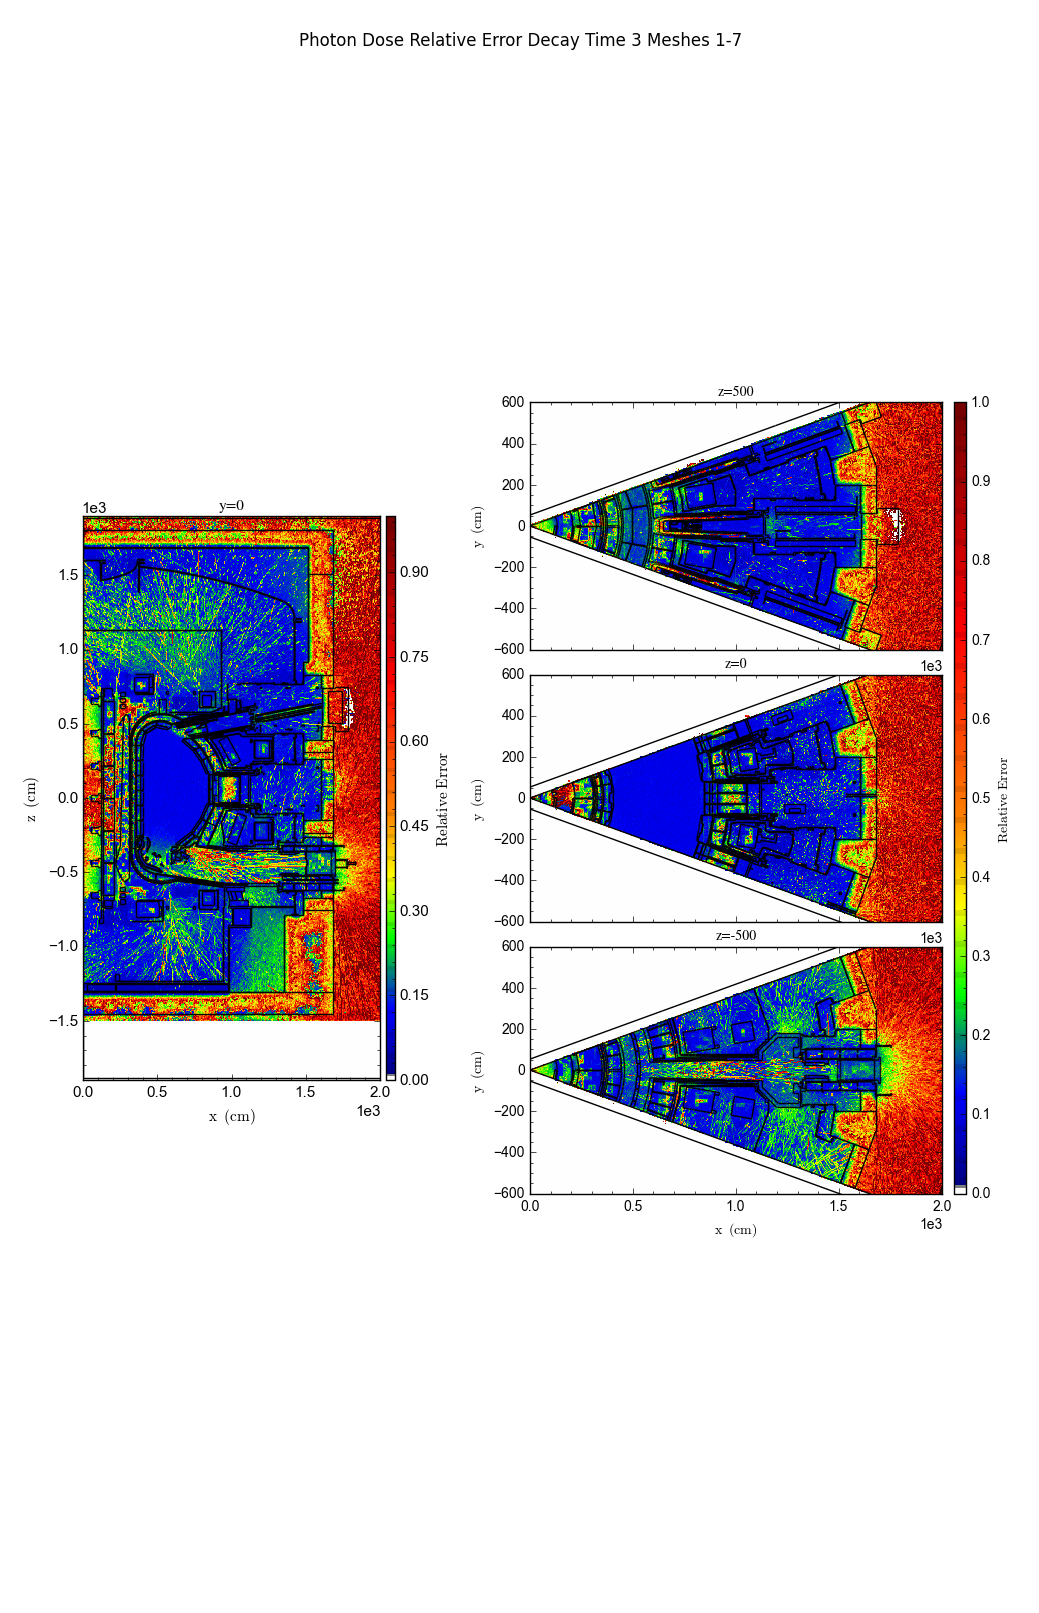
\includegraphics[trim={0cm 8cm, 0cm 8cm},clip,scale=0.75]{../plots/final_model_with_b4c/5year/Photon_Dose_Relative_Error_Decay_Time_3_Meshes_1-7.png}
\caption{Total dose rate relative error for decay time 3 for the 5 year irradiation}
\label{fig:photons_5y_dc3_nob4c_relerr}
\end{figure}
\clearpage
\newpage
\section{Appendix B - B4C 10 Year Irradiation}
\begin{figure}[ht!]
\centering
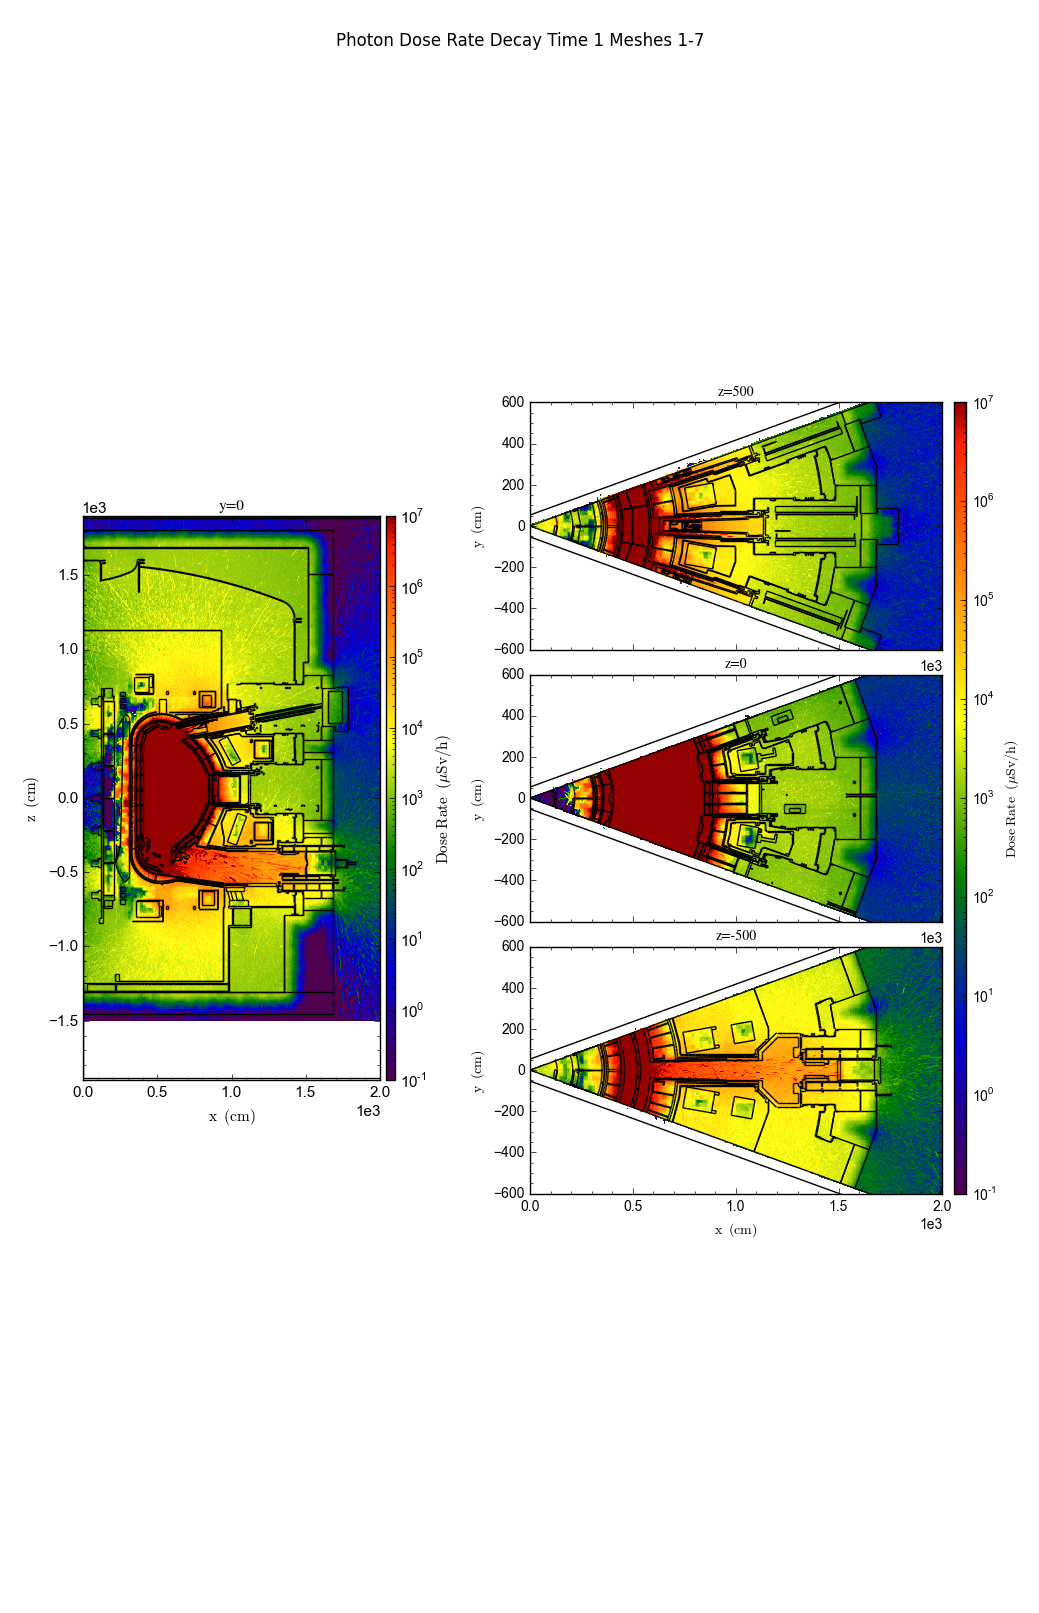
\includegraphics[trim={0cm 8cm, 0cm 8cm},clip,scale=0.75]{../plots/final_model_with_b4c/10year/Photon_Dose_Rate_Decay_Time_1_Meshes_1-7.png}
\caption{Total dose rate for decay time 1 for the 10 year irradiation}
\label{fig:photons_10y_dc1_nob4c_dose}
\end{figure}
\begin{figure}[ht!]
\centering
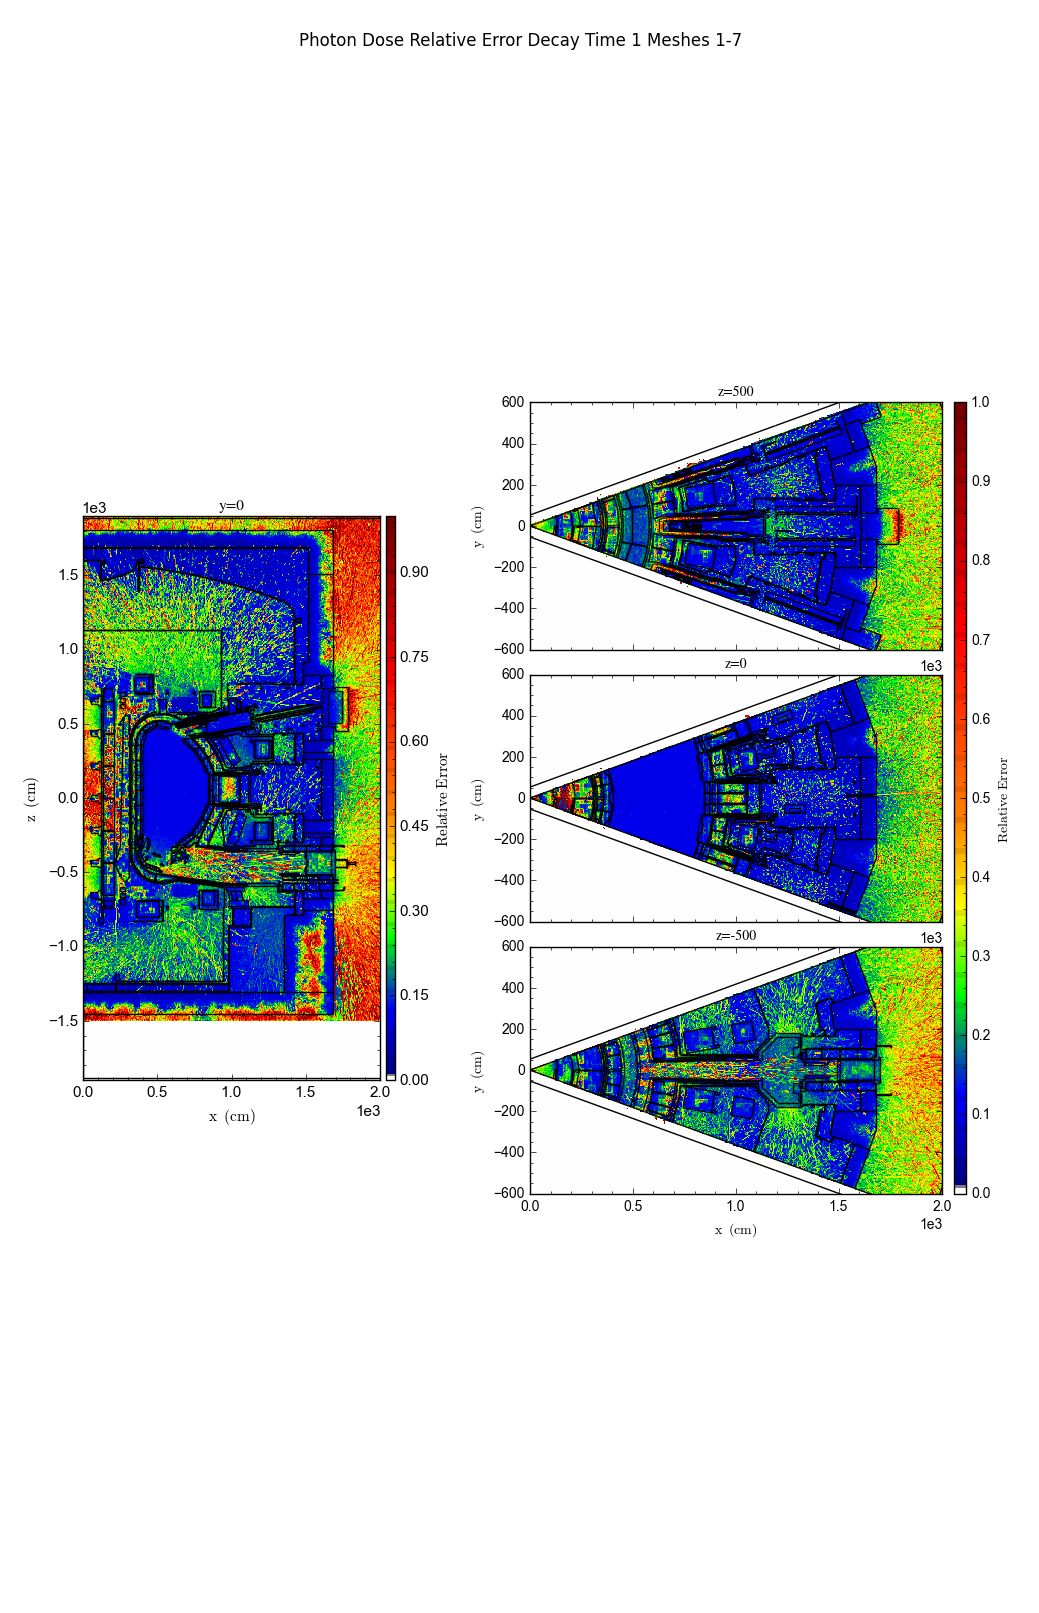
\includegraphics[trim={0cm 8cm, 0cm 8cm},clip,scale=0.75]{../plots/final_model_with_b4c/10year/Photon_Dose_Relative_Error_Decay_Time_1_Meshes_1-7.png}
\caption{Total dose rate relative error for decay time 1 for the 10 year irradiation}
\label{fig:photons_10y_dc1_nob4c_relerr}
\end{figure}
\clearpage
\begin{figure}[ht!]
\centering
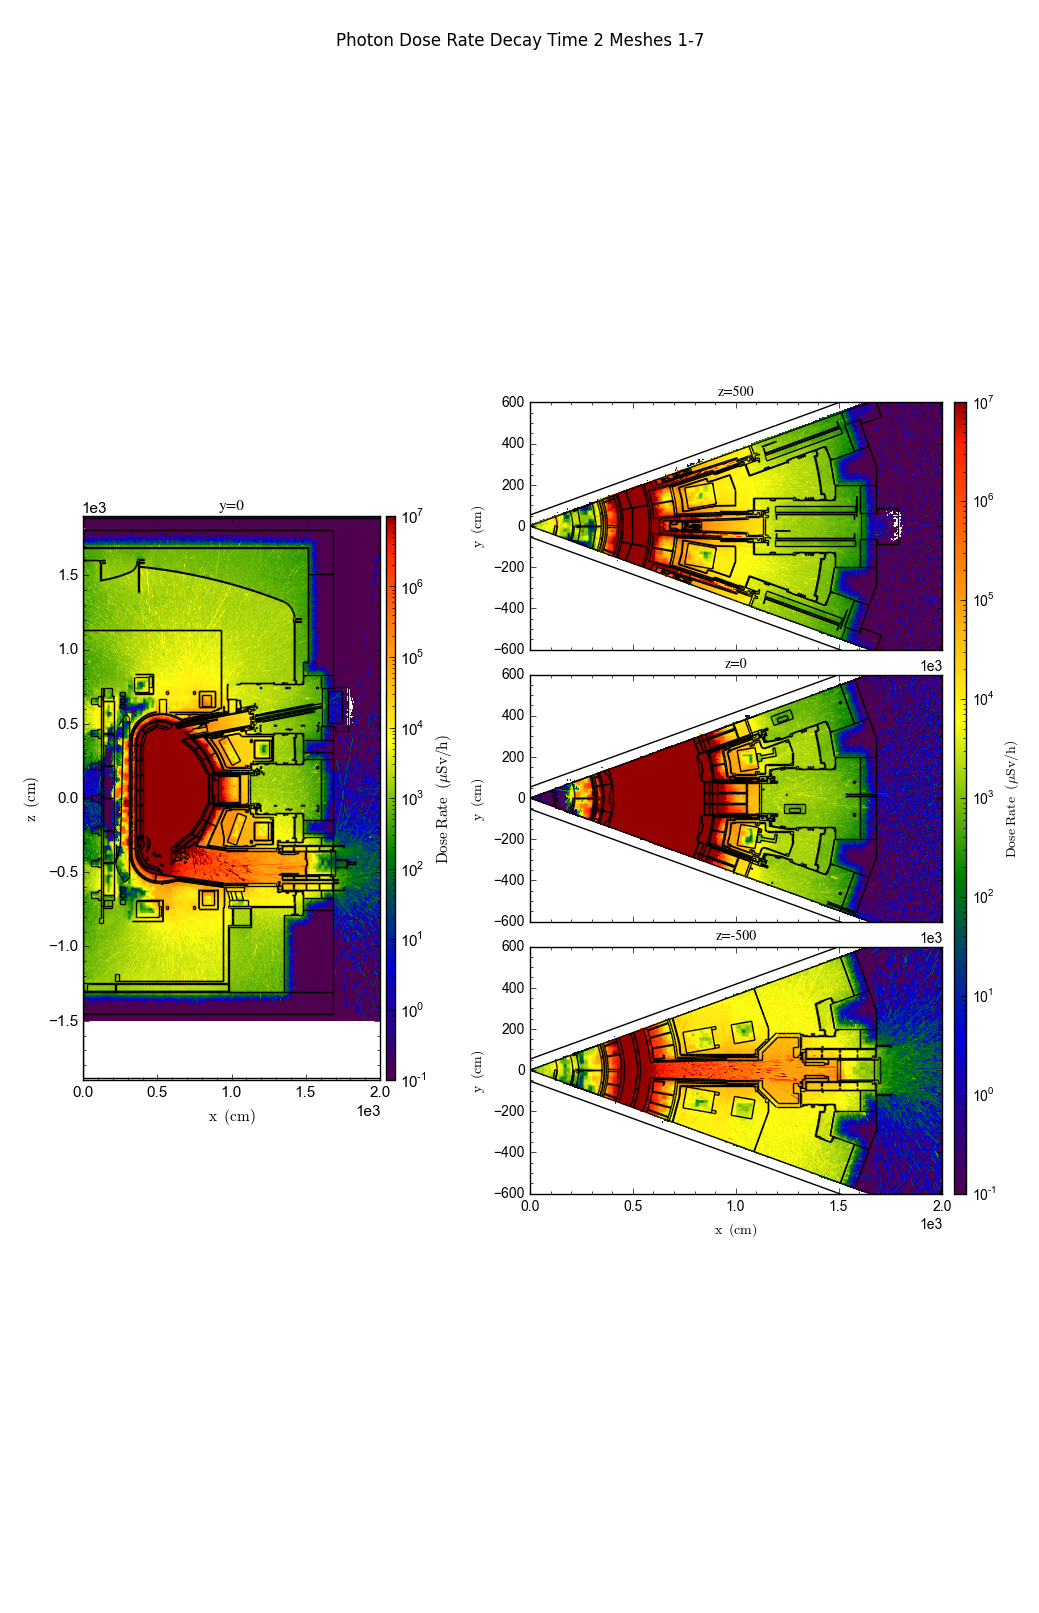
\includegraphics[trim={0cm 8cm, 0cm 8cm},clip,scale=0.75]{../plots/final_model_with_b4c/10year/Photon_Dose_Rate_Decay_Time_2_Meshes_1-7.png}
\caption{Total dose rate for decay time 2 for the 10 year irradiation}
\label{fig:photons_10y_dc2_nob4c_dose}
\end{figure}
\begin{figure}[ht!]
\centering
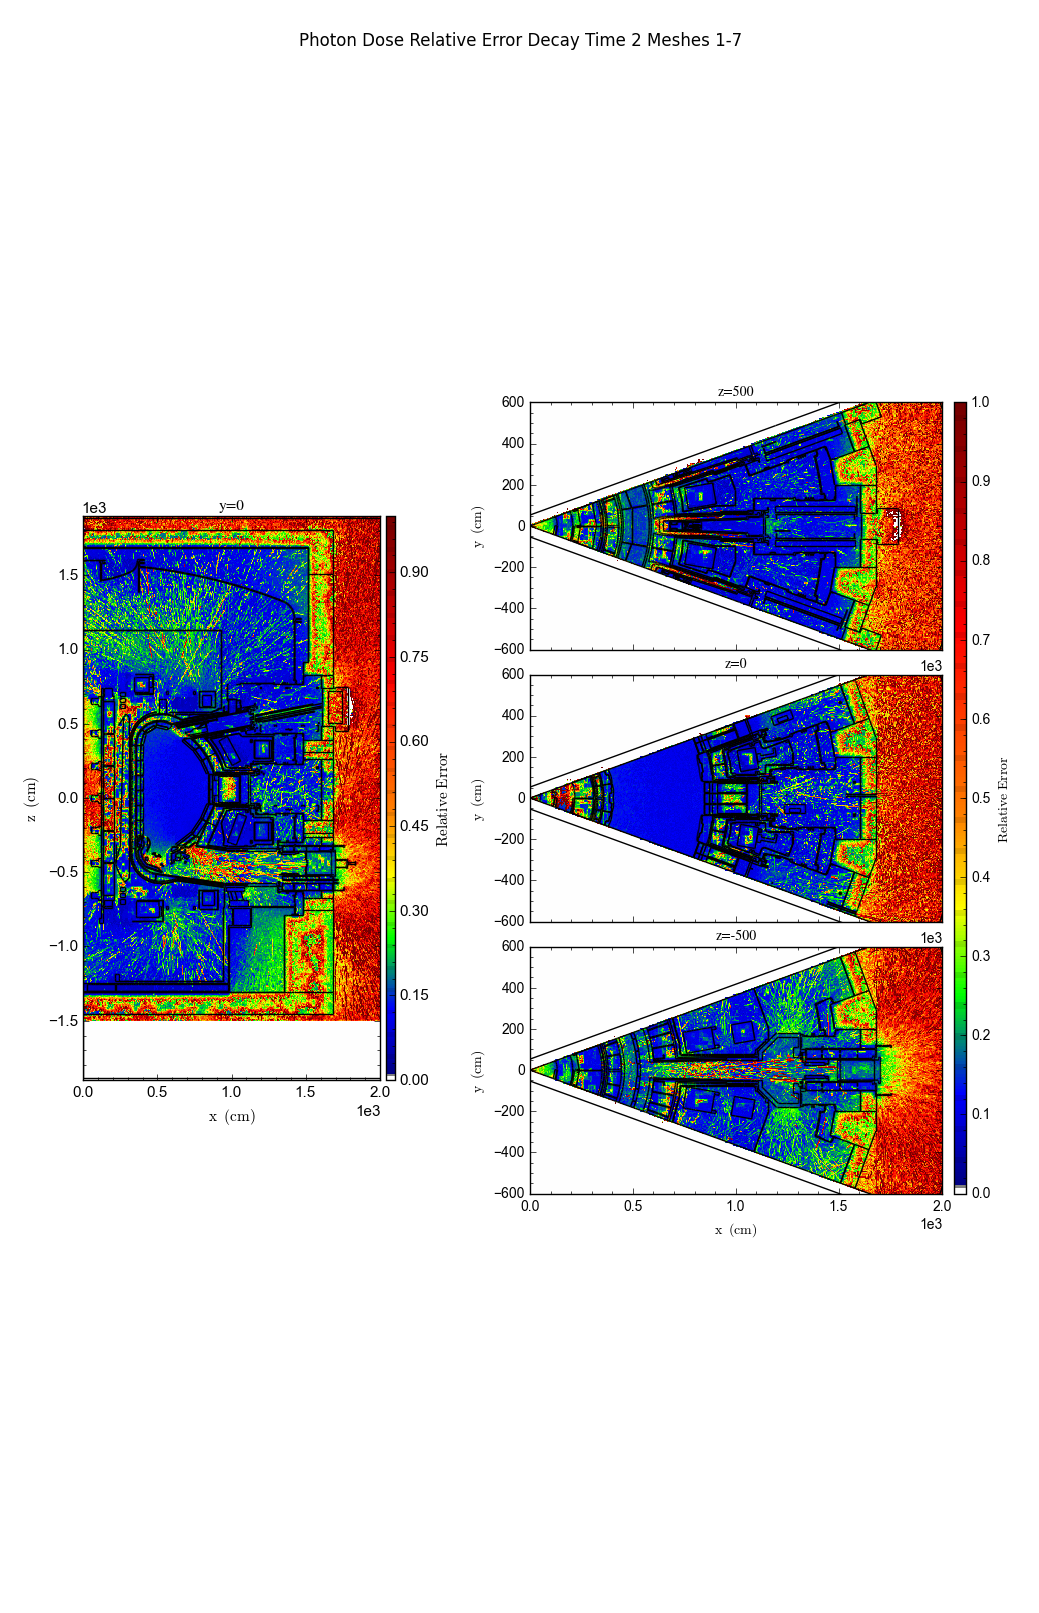
\includegraphics[trim={0cm 8cm, 0cm 8cm},clip,scale=0.75]{../plots/final_model_with_b4c/10year/Photon_Dose_Relative_Error_Decay_Time_2_Meshes_1-7.png}
\caption{Total dose rate relative error for decay time 2 for the 10 year irradiation}
\label{fig:photons_10y_dc2_nob4c_relerr}
\end{figure}

\clearpage
\begin{figure}[ht!]
\centering
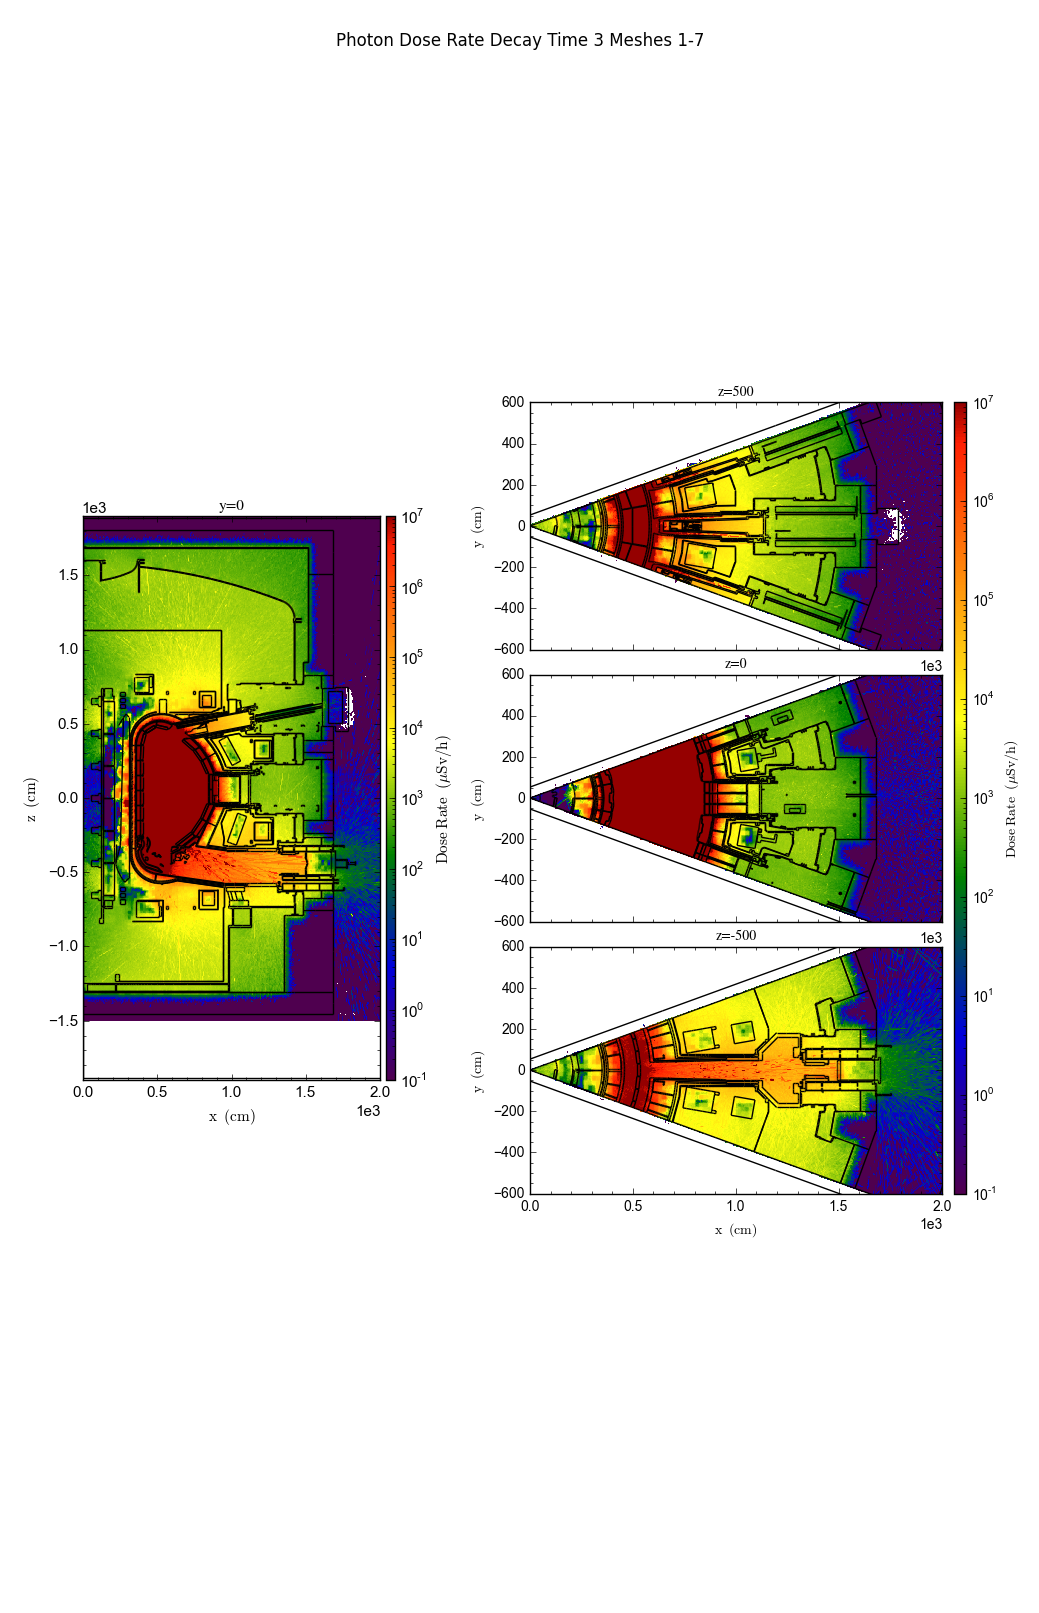
\includegraphics[trim={0cm 8cm, 0cm 8cm},clip,scale=0.75]{../plots/final_model_with_b4c/10year/Photon_Dose_Rate_Decay_Time_3_Meshes_1-7.png}
\caption{Total dose rate for decay time 3 for the 10 year irradiation}
\label{fig:photons_10y_dc2_nob4c_dose}
\end{figure}
\begin{figure}[ht!]
\centering
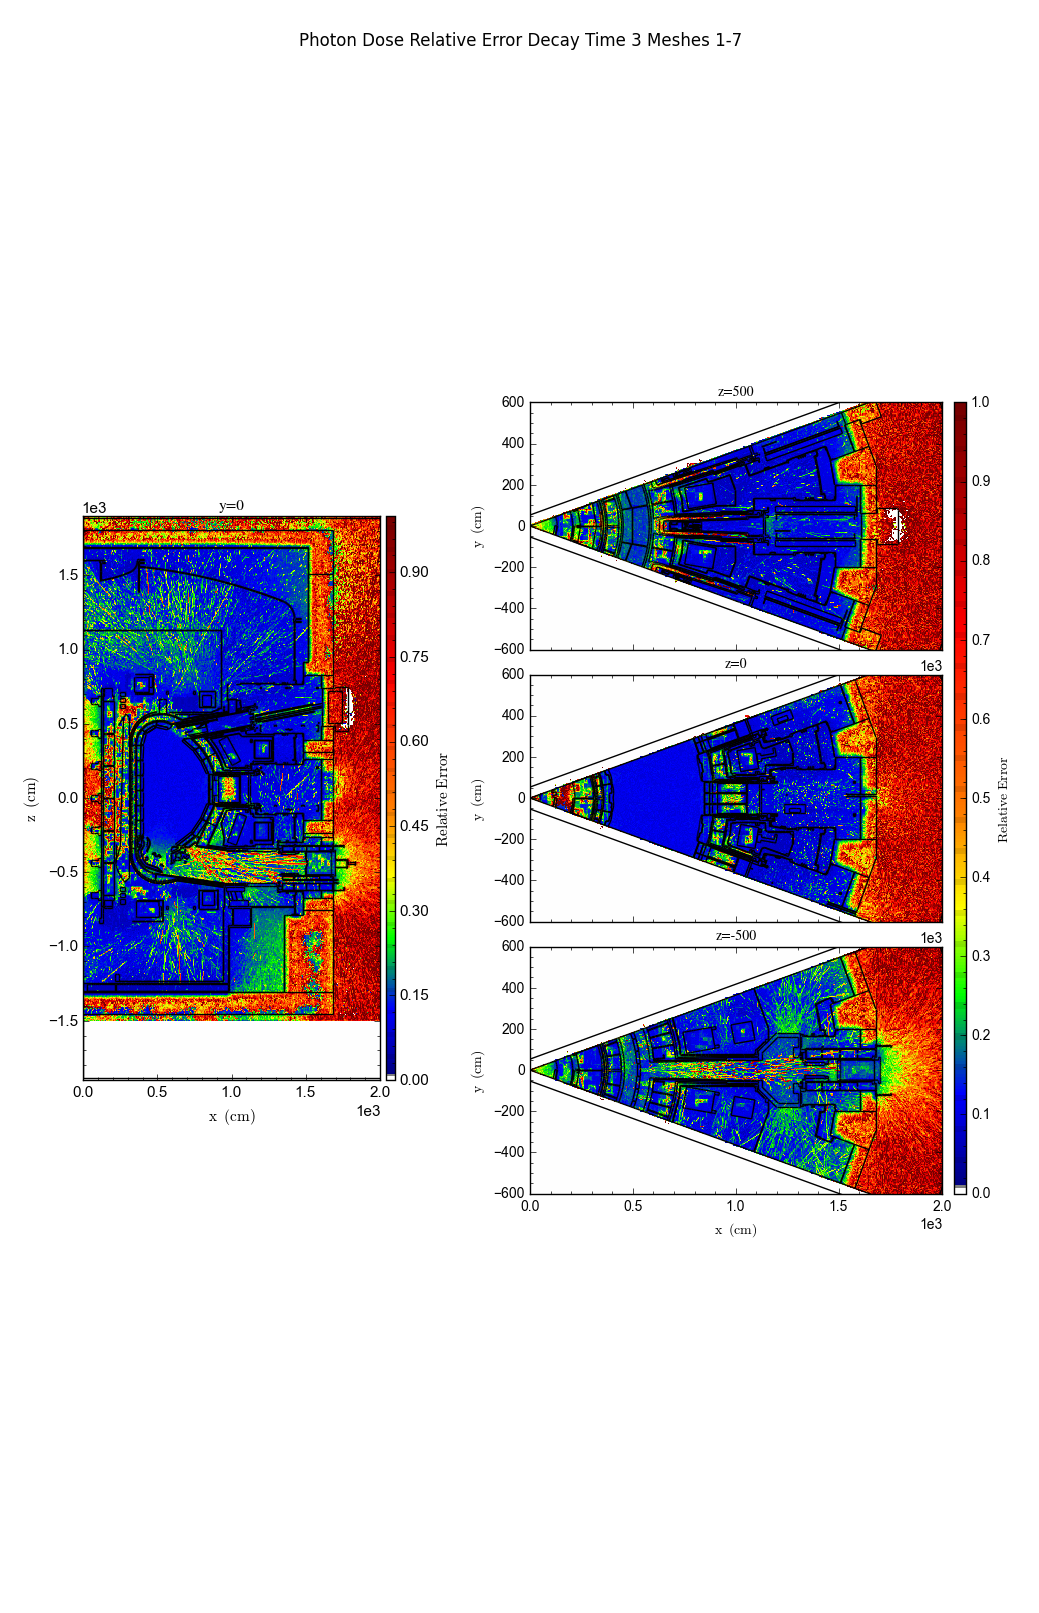
\includegraphics[trim={0cm 8cm, 0cm 8cm},clip,scale=0.75]{../plots/final_model_with_b4c/10year/Photon_Dose_Relative_Error_Decay_Time_3_Meshes_1-7.png}
\caption{Total dose rate relative error for decay time 3 for the 10 year irradiation}
\label{fig:photons_10y_dc3_nob4c_relerr}
\end{figure}
\newpage
\section{Appendix C - No B4C 5 Year Irradiation}
\begin{figure}[ht!]
\centering
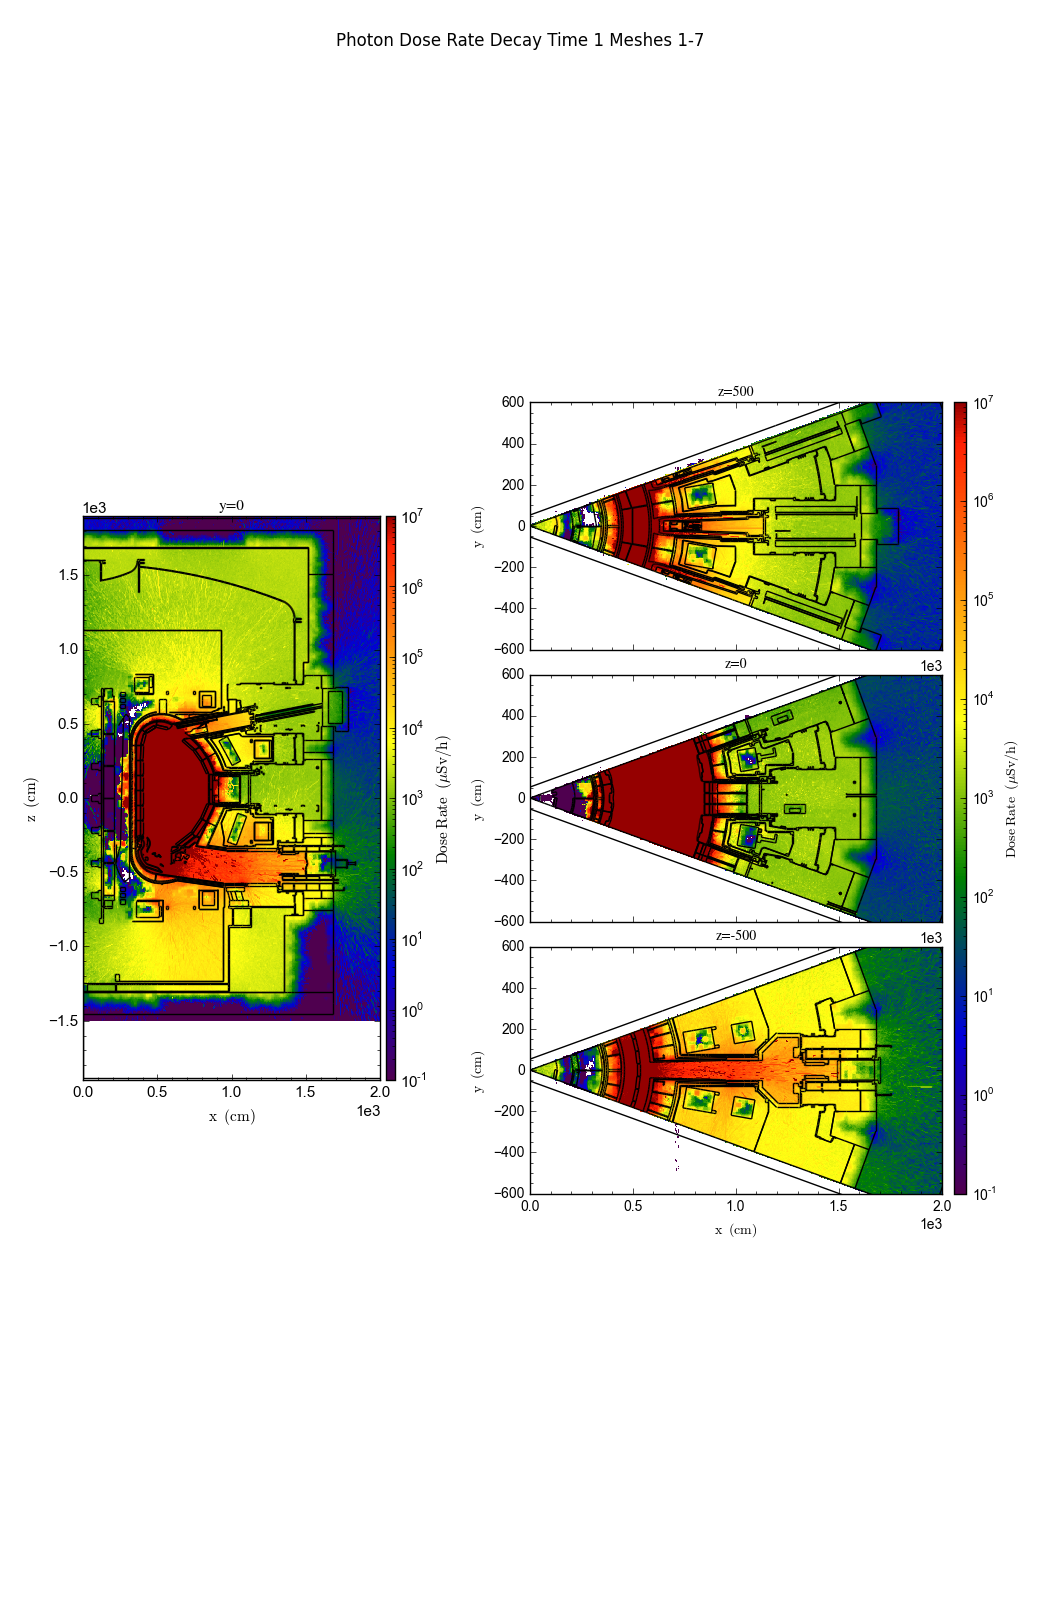
\includegraphics[trim={0cm 8cm, 0cm 8cm},clip,scale=0.75]{../plots/final_model/5year/Photon_Dose_Rate_Decay_Time_1_Meshes_1-7.png}
\caption{Total dose rate for decay time 1 for the 5 year irradiation}
\label{fig:photons_5y_dc1_nob4c_dose}
\end{figure}
\begin{figure}[ht!]
\centering
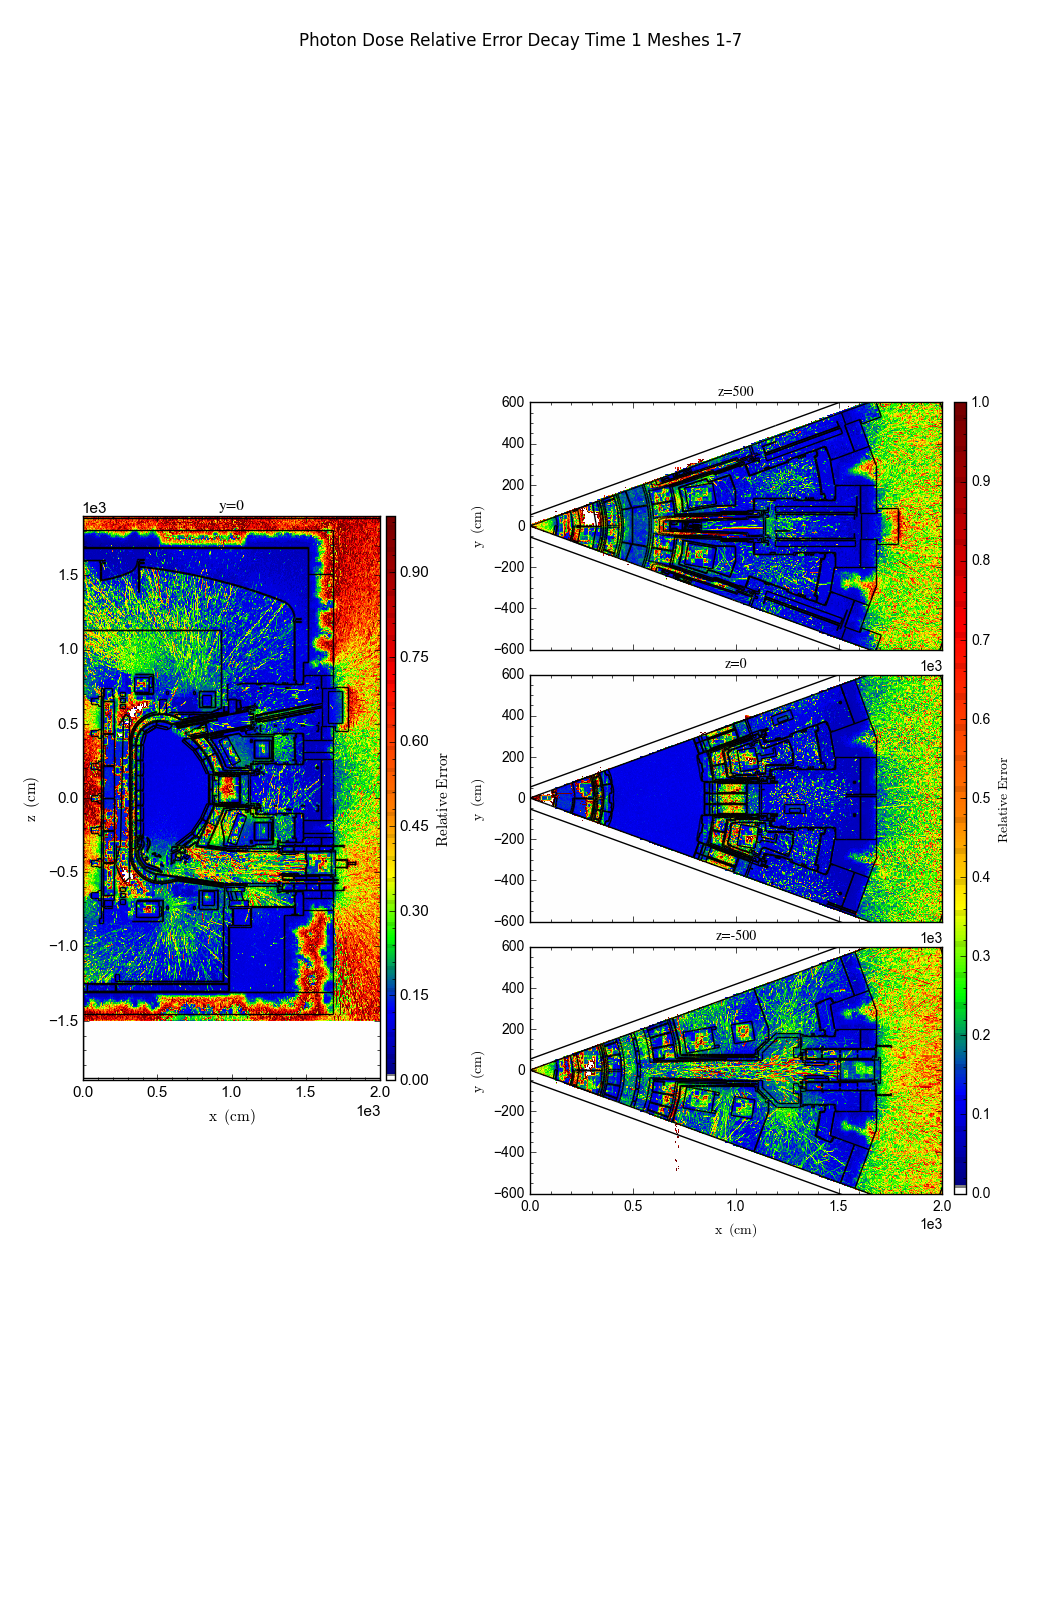
\includegraphics[trim={0cm 8cm, 0cm 8cm},clip,scale=0.75]{../plots/final_model/5year/Photon_Dose_Relative_Error_Decay_Time_1_Meshes_1-7.png}
\caption{Total dose rate relative error for decay time 1 for the 5 year irradiation}
\label{fig:photons_5y_dc1_nob4c_relerr}
\end{figure}
\clearpage
\begin{figure}[ht!]
\centering
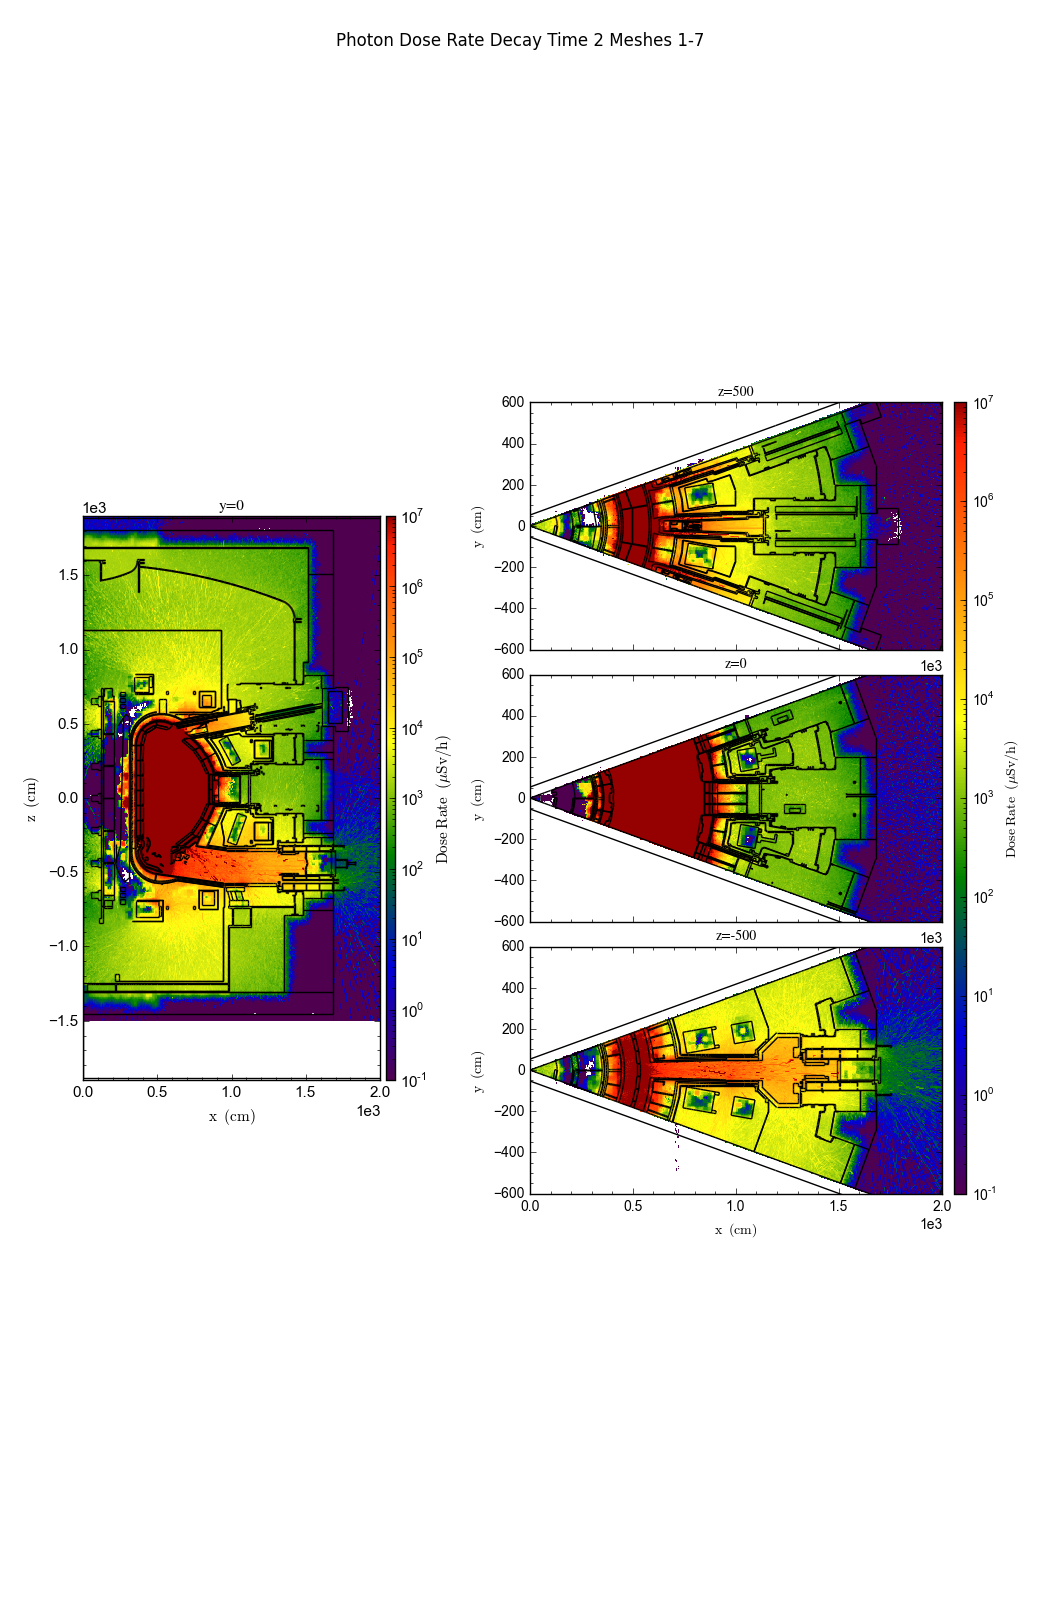
\includegraphics[trim={0cm 8cm, 0cm 8cm},clip,scale=0.75]{../plots/final_model/5year/Photon_Dose_Rate_Decay_Time_2_Meshes_1-7.png}
\caption{Total dose rate for decay time 2 for the 5 year irradiation}
\label{fig:photons_5y_dc2_nob4c_dose}
\end{figure}
\begin{figure}[ht!]
\centering
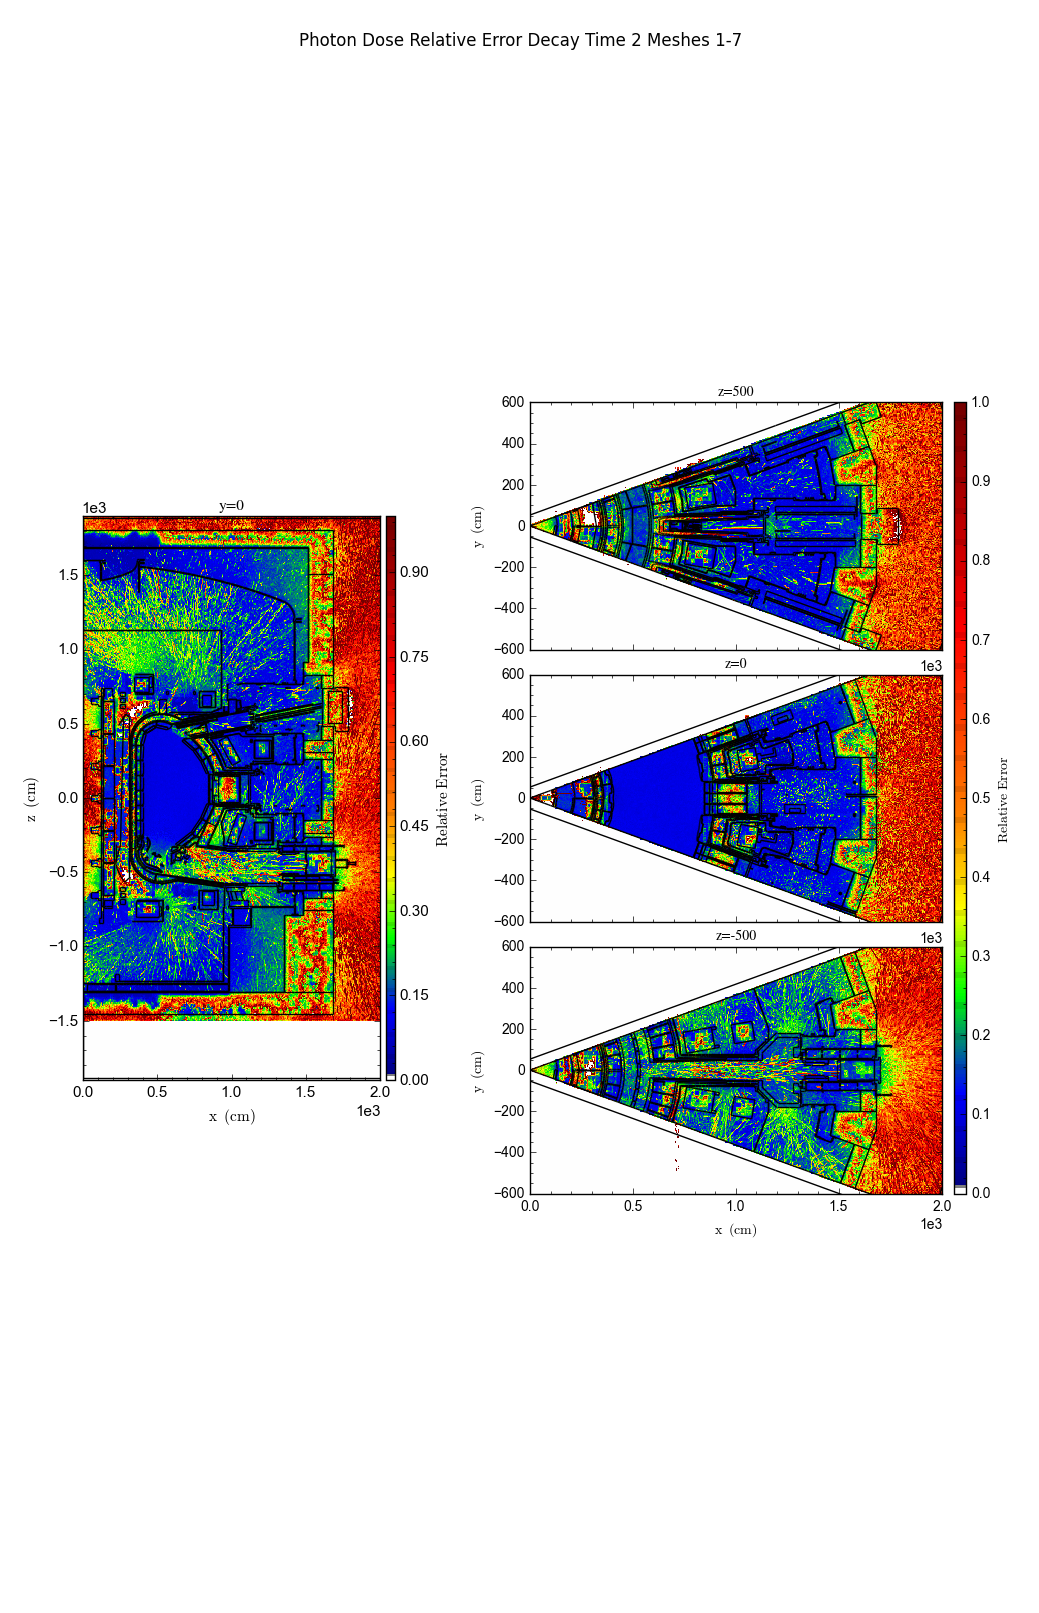
\includegraphics[trim={0cm 8cm, 0cm 8cm},clip,scale=0.75]{../plots/final_model/5year/Photon_Dose_Relative_Error_Decay_Time_2_Meshes_1-7.png}
\caption{Total dose rate relative error for decay time 2 for the 5 year irradiation}
\label{fig:photons_5y_dc2_nob4c_relerr}
\end{figure}
\clearpage
\begin{figure}[ht!]
\centering
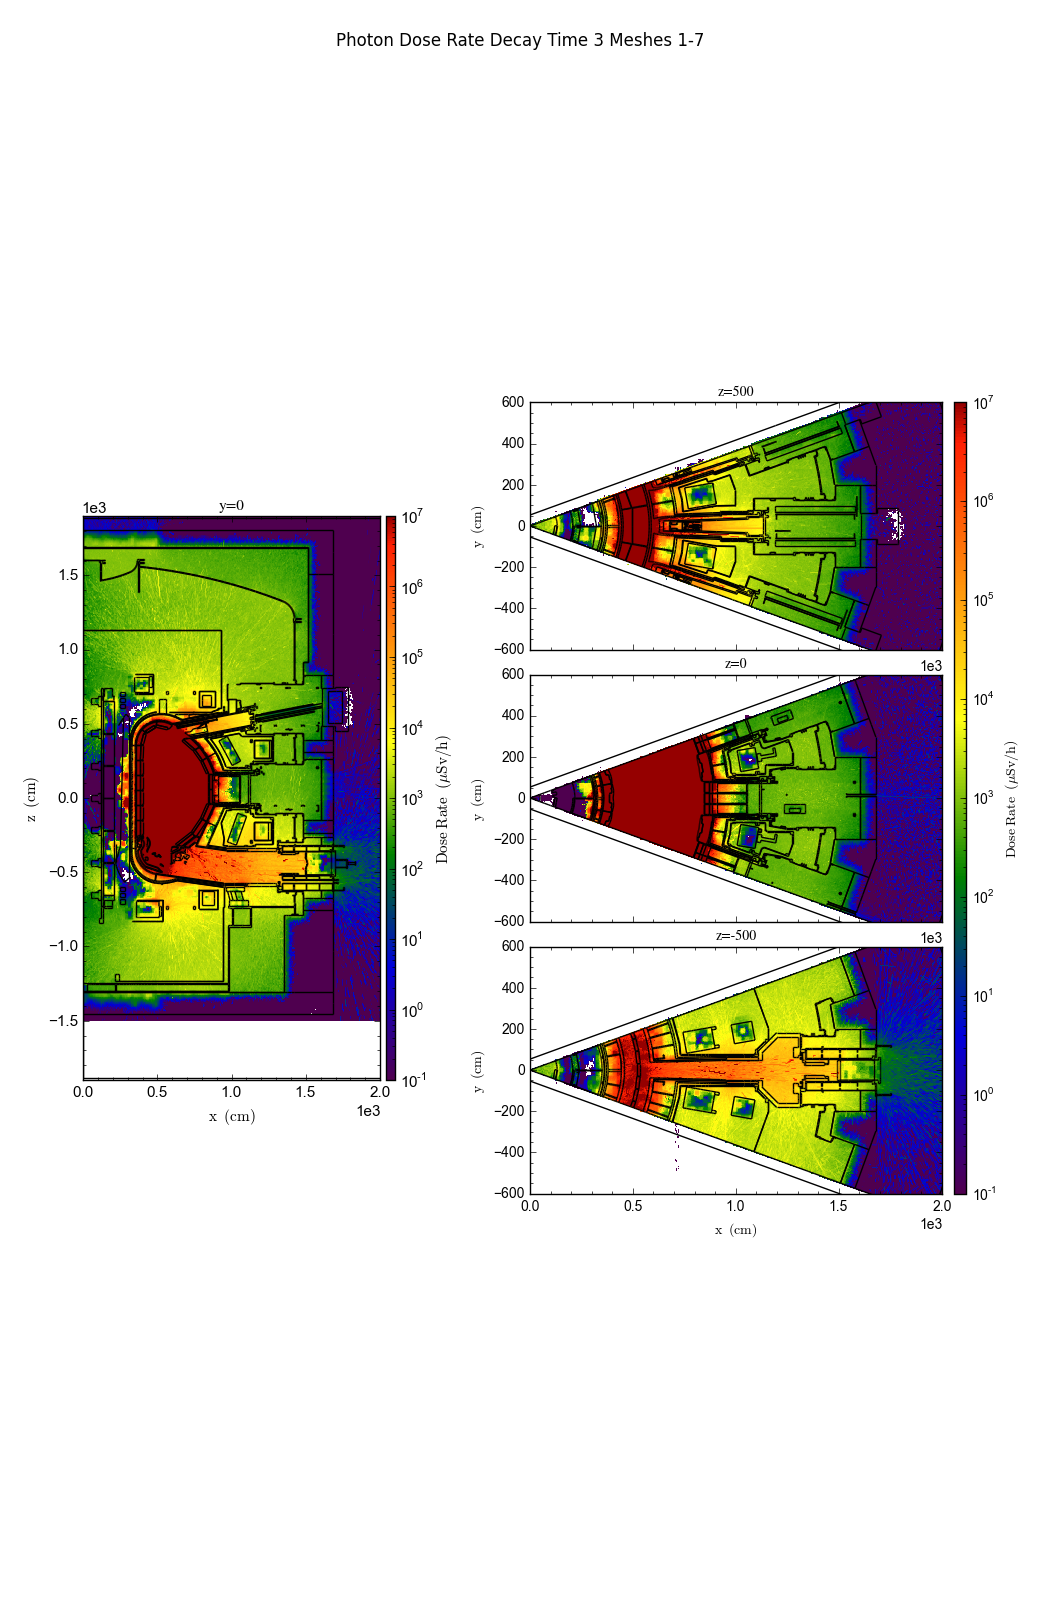
\includegraphics[trim={0cm 8cm, 0cm 8cm},clip,scale=0.75]{../plots/final_model/5year/Photon_Dose_Rate_Decay_Time_3_Meshes_1-7.png}
\caption{Total dose rate for decay time 3 for the 5 year irradiation}
\label{fig:photons_5y_dc3_nob4c_dose}
\end{figure}
\begin{figure}[ht!]
\centering
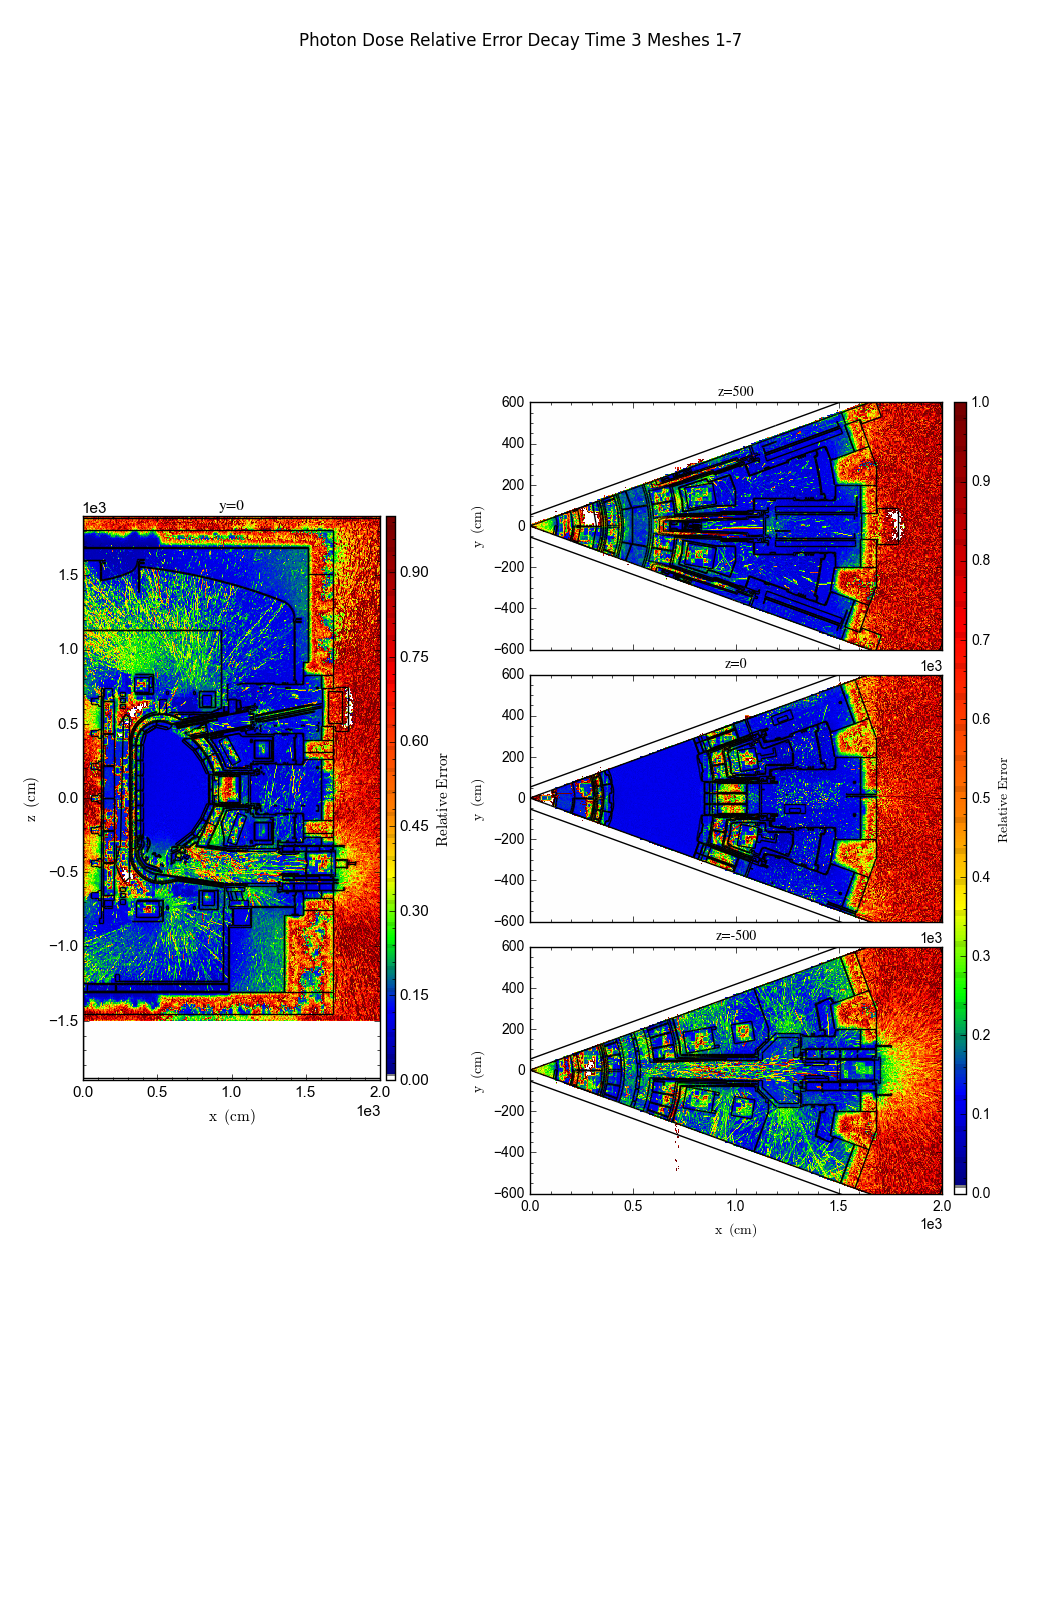
\includegraphics[trim={0cm 8cm, 0cm 8cm},clip,scale=0.75]{../plots/final_model/5year/Photon_Dose_Relative_Error_Decay_Time_3_Meshes_1-7.png}
\caption{Total dose rate relative error for decay time 3 for the 5 year irradiation}
\label{fig:photons_5y_dc3_nob4c_relerr}
\end{figure}
\clearpage
\newpage
\section{Appendix D - No B4C 10 Year Irradiation}
\begin{figure}[ht!]
\centering
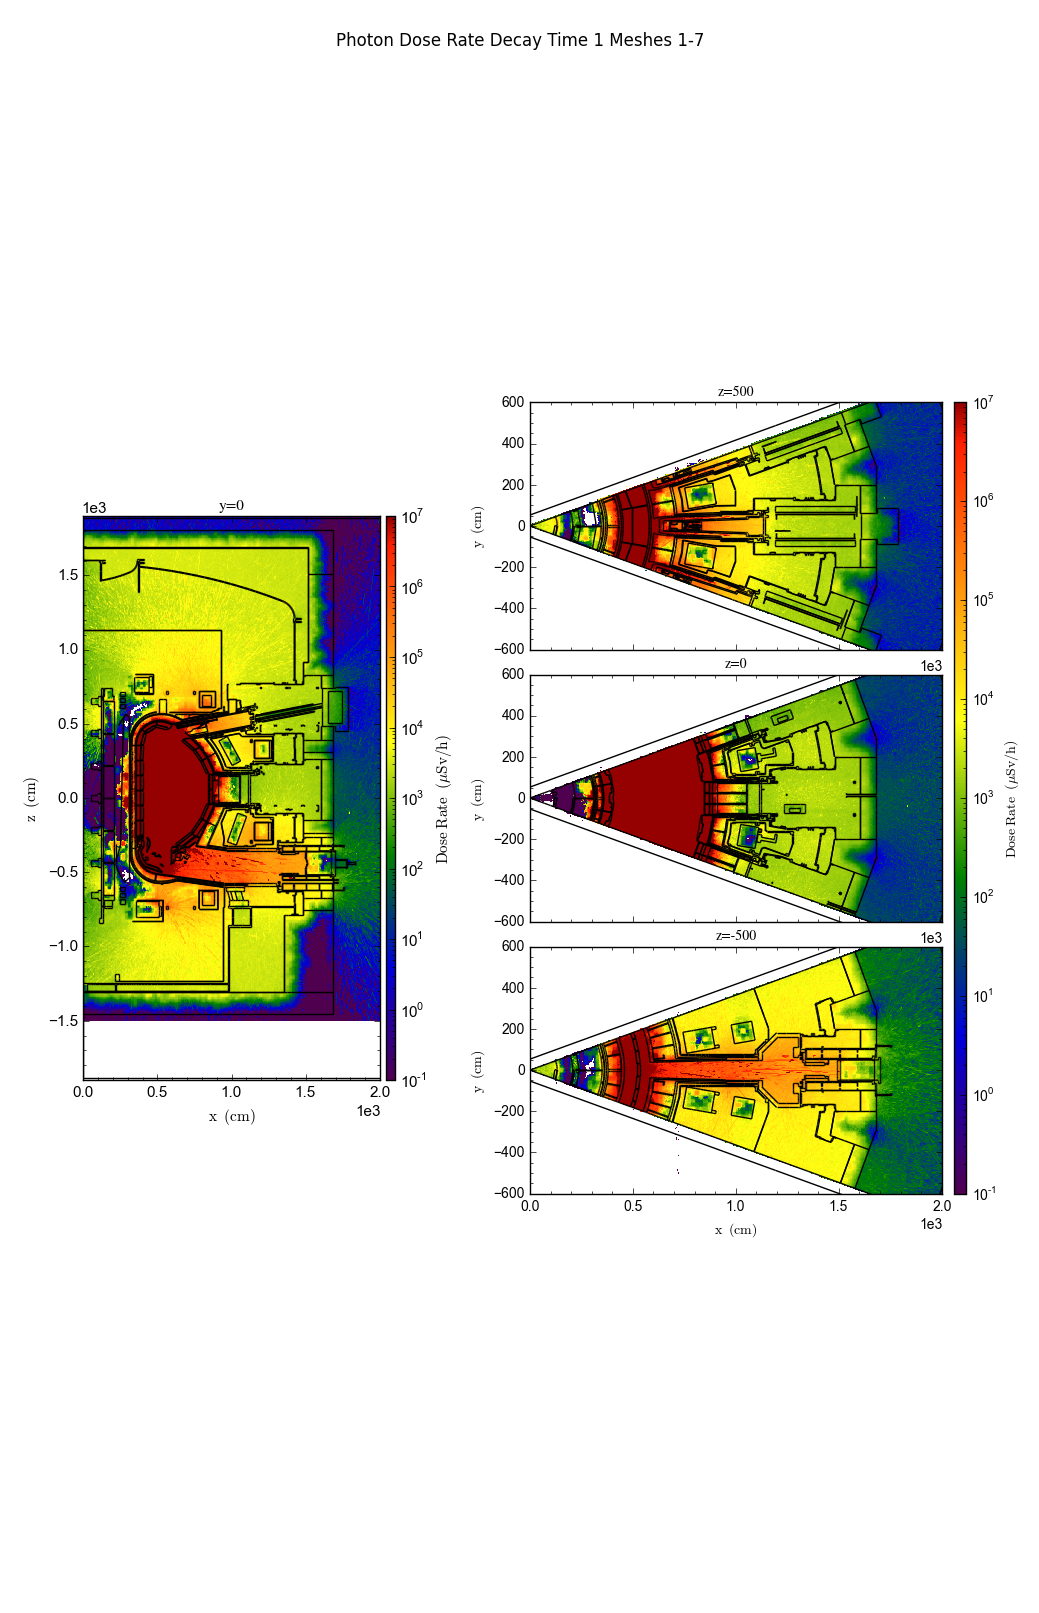
\includegraphics[trim={0cm 8cm, 0cm 8cm},clip,scale=0.75]{../plots/final_model/10year/Photon_Dose_Rate_Decay_Time_1_Meshes_1-7.png}
\caption{Total dose rate for decay time 1 for the 10 year irradiation}
\label{fig:photons_10y_dc1_nob4c_dose}
\end{figure}
\begin{figure}[ht!]
\centering
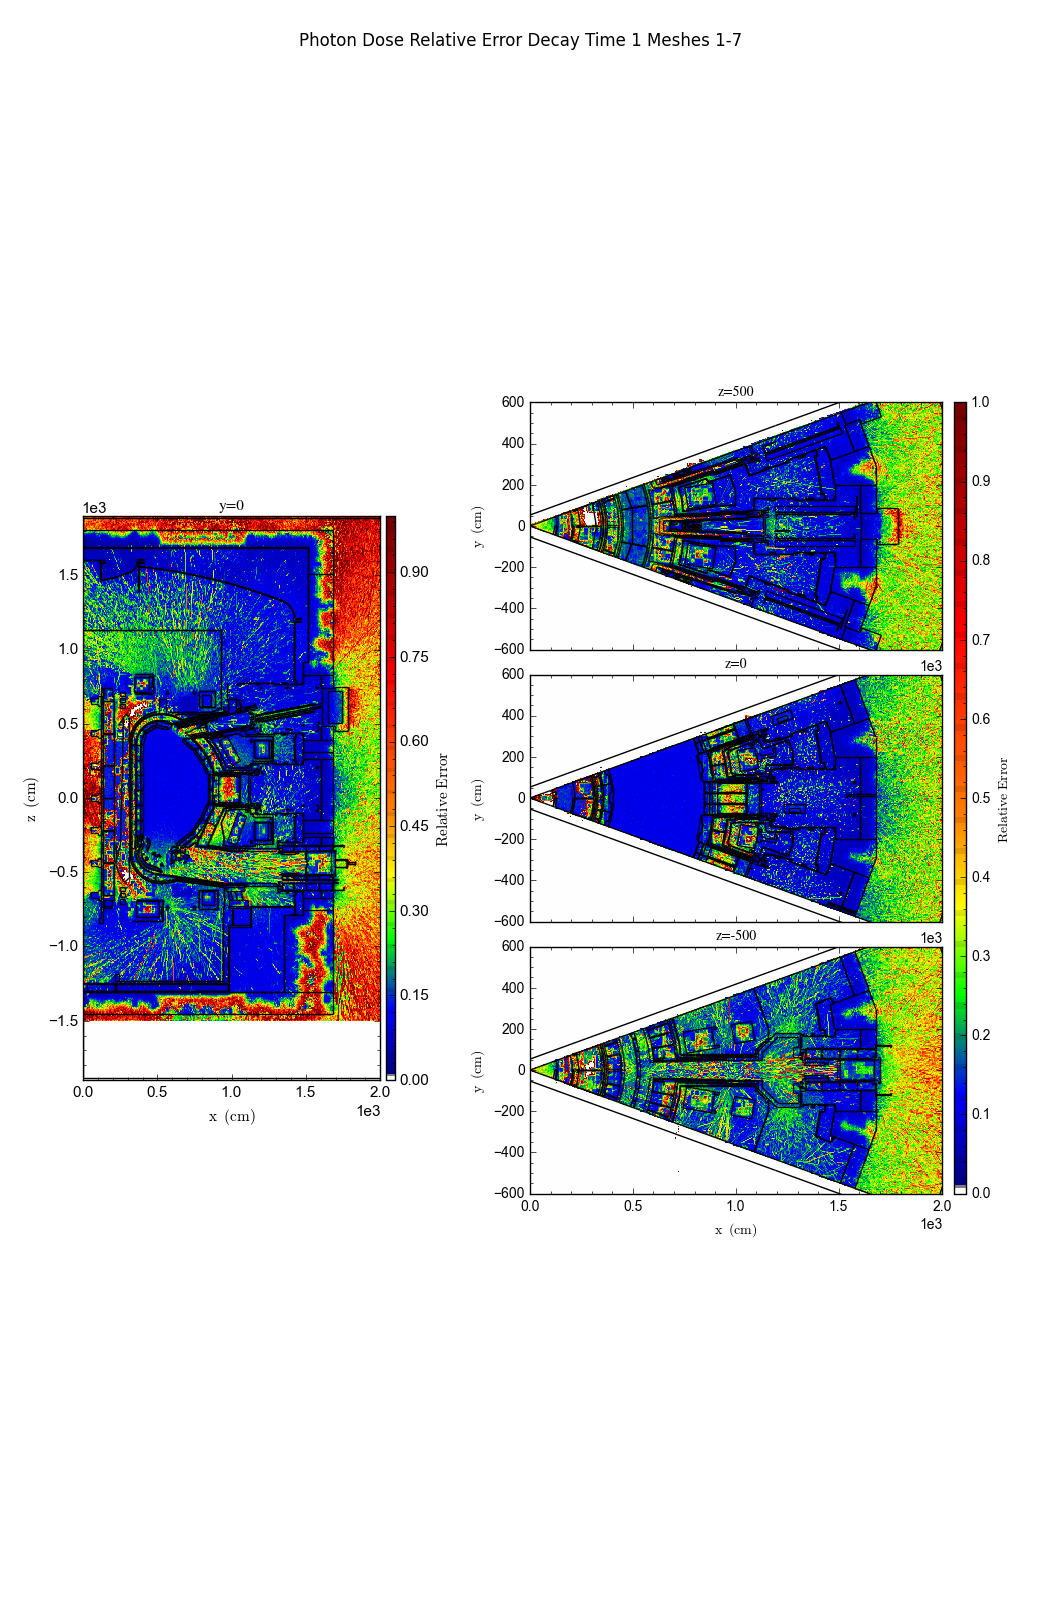
\includegraphics[trim={0cm 8cm, 0cm 8cm},clip,scale=0.75]{../plots/final_model/10year/Photon_Dose_Relative_Error_Decay_Time_1_Meshes_1-7.png}
\caption{Total dose rate relative error for decay time 1 for the 10 year irradiation}
\label{fig:photons_10y_dc1_nob4c_relerr}
\end{figure}
\clearpage
\begin{figure}[ht!]
\centering
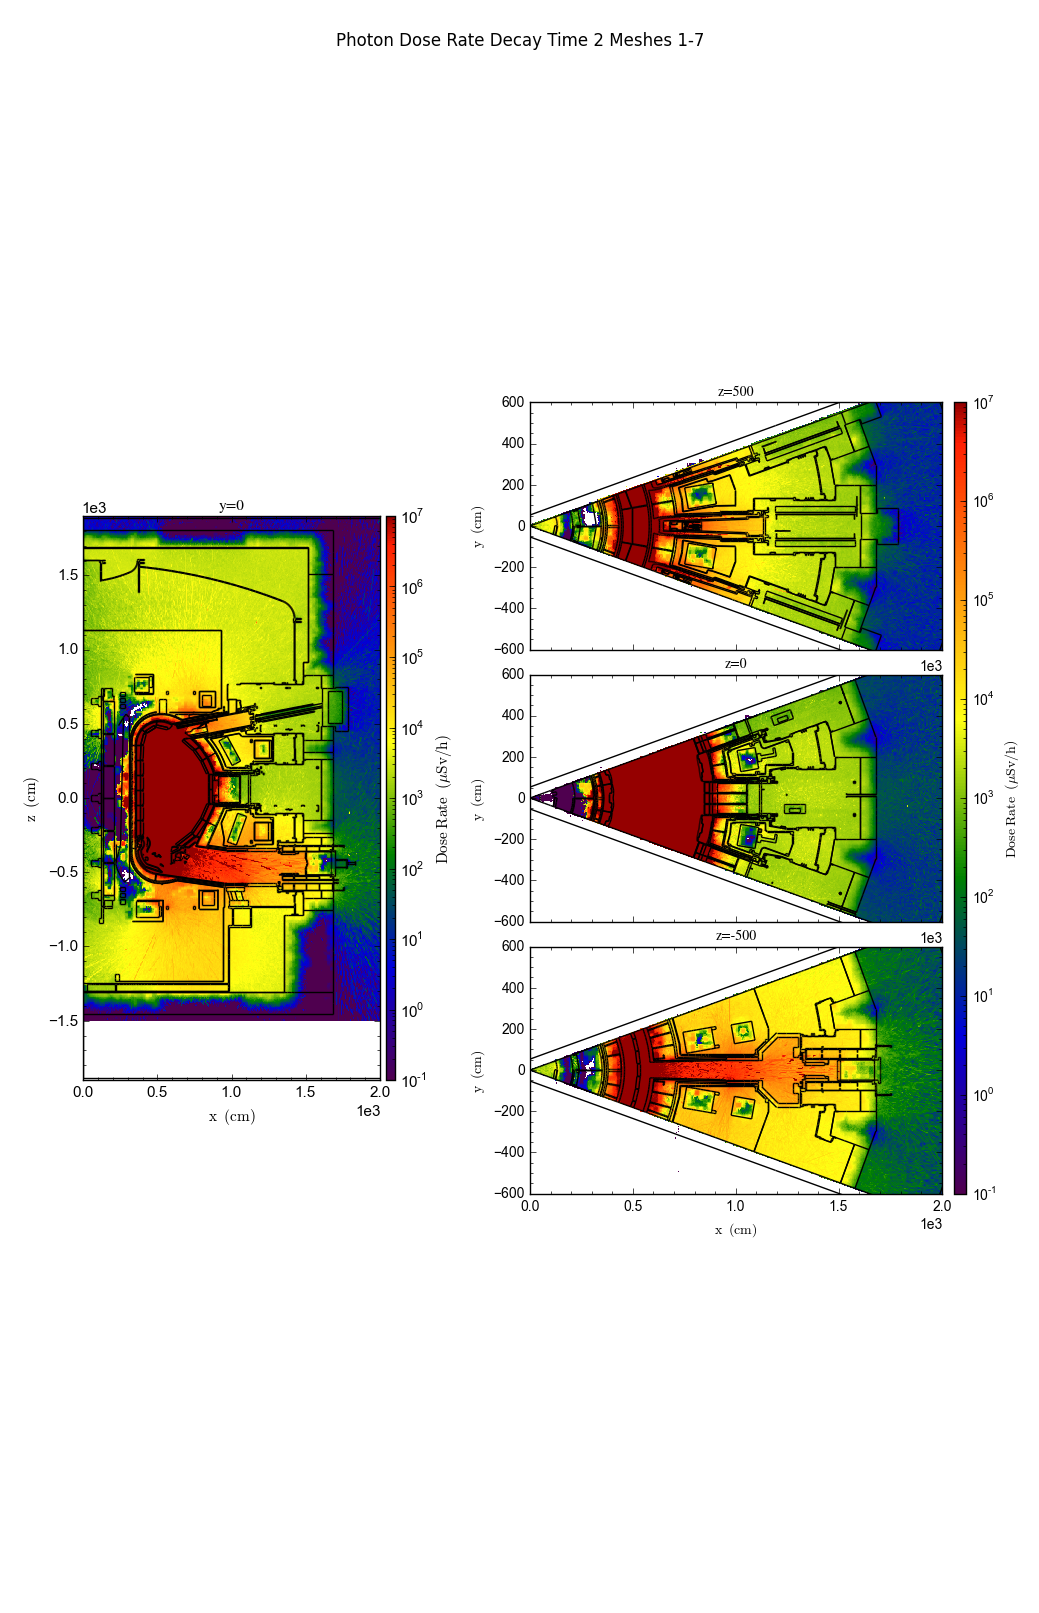
\includegraphics[trim={0cm 8cm, 0cm 8cm},clip,scale=0.75]{../plots/final_model/10year/Photon_Dose_Rate_Decay_Time_2_Meshes_1-7.png}
\caption{Total dose rate for decay time 2 for the 10 year irradiation}
\label{fig:photons_10y_dc2_nob4c_dose}
\end{figure}
\begin{figure}[ht!]
\centering
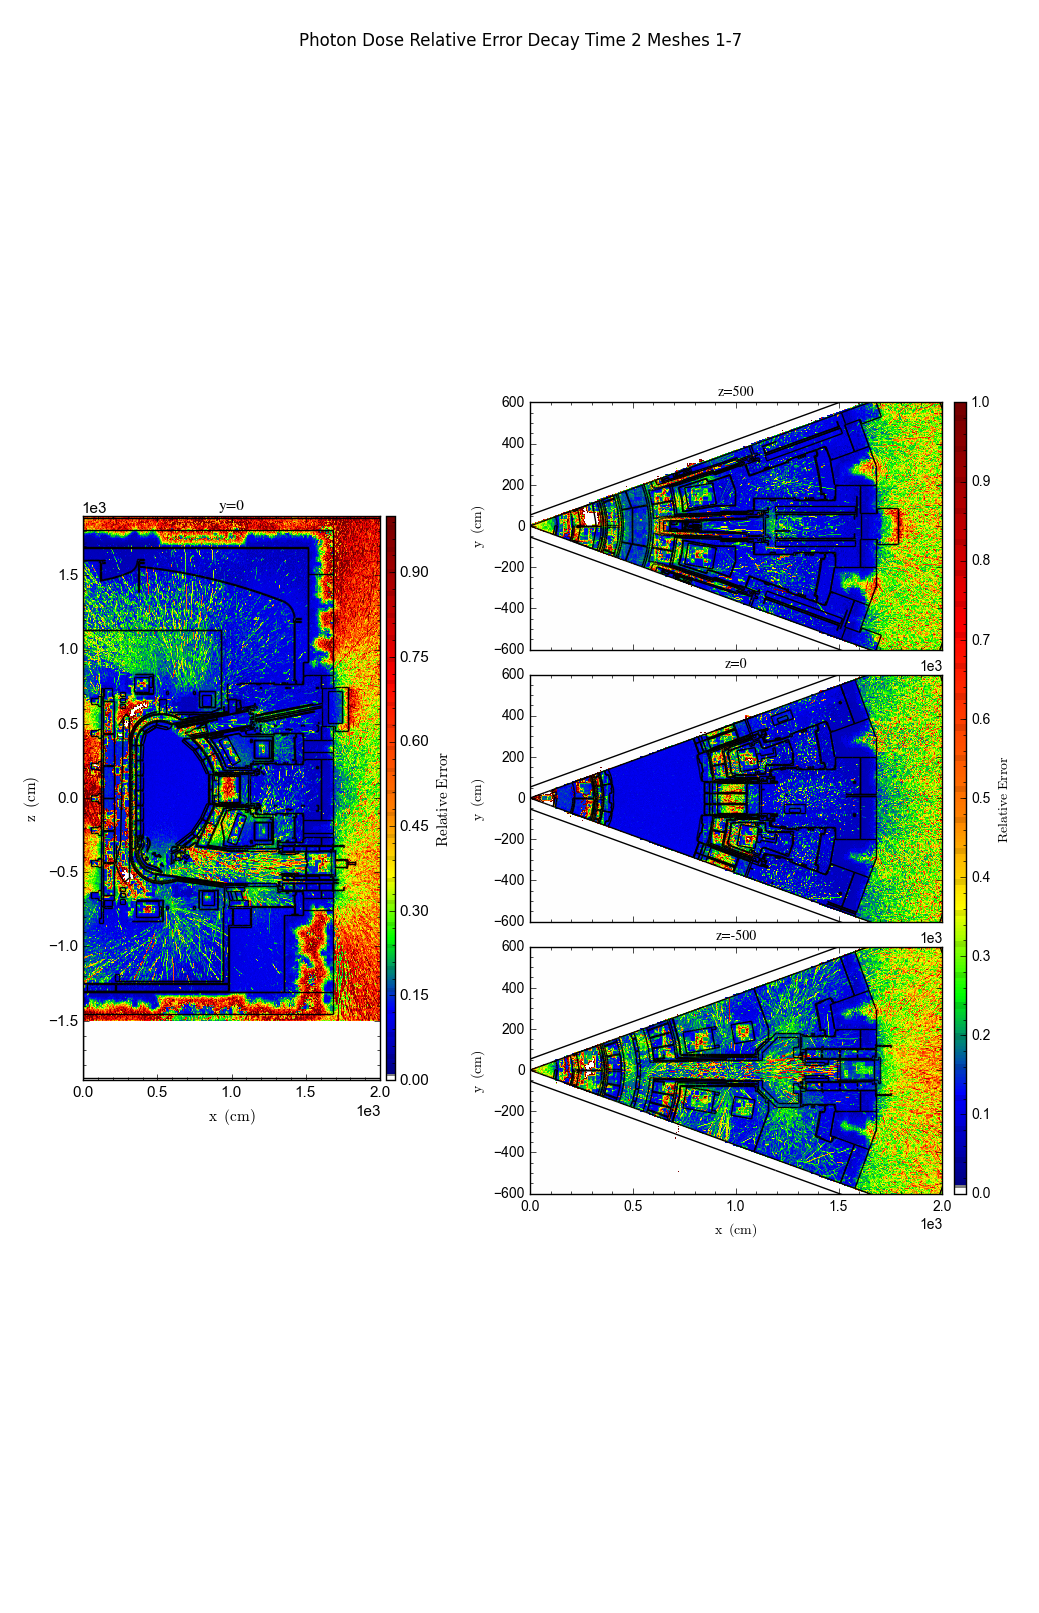
\includegraphics[trim={0cm 8cm, 0cm 8cm},clip,scale=0.75]{../plots/final_model/10year/Photon_Dose_Relative_Error_Decay_Time_2_Meshes_1-7.png}
\caption{Total dose rate relative error for decay time 2 for the 10 year irradiation}
\label{fig:photons_10y_dc2_nob4c_relerr}
\end{figure}

\clearpage
\begin{figure}[ht!]
\centering
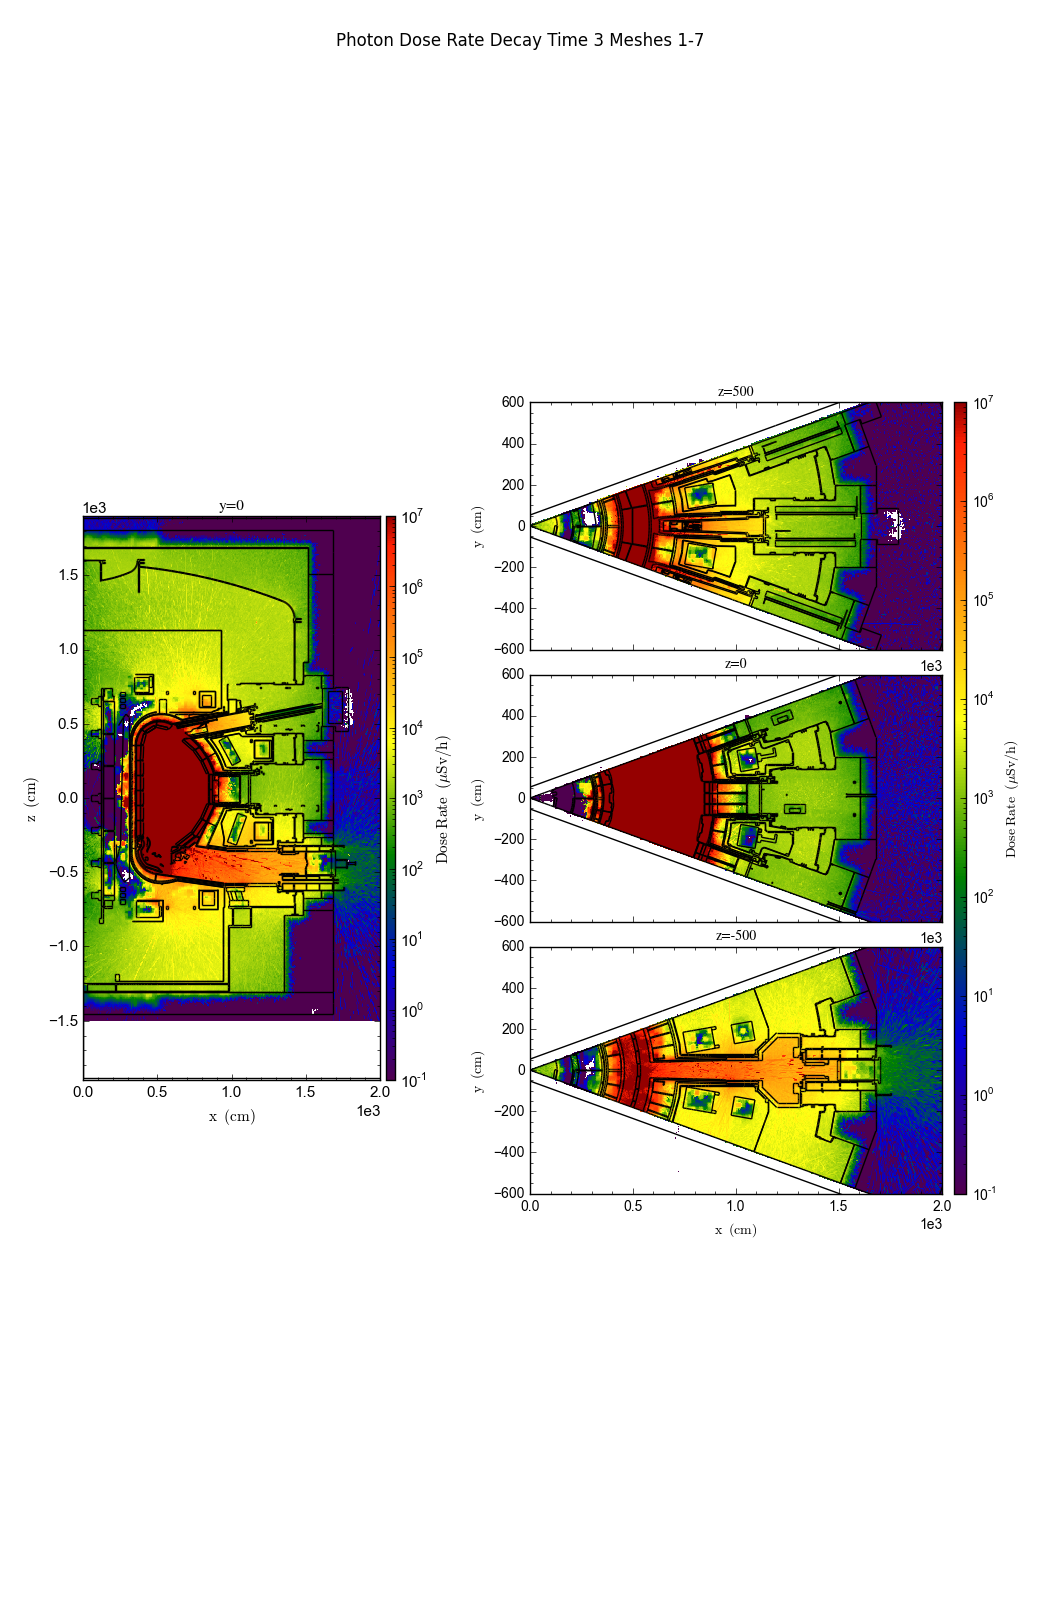
\includegraphics[trim={0cm 8cm, 0cm 8cm},clip,scale=0.75]{../plots/final_model/10year/Photon_Dose_Rate_Decay_Time_3_Meshes_1-7.png}
\caption{Total dose rate for decay time 3 for the 10 year irradiation}
\label{fig:photons_10y_dc2_nob4c_dose}
\end{figure}
\begin{figure}[ht!]
\centering
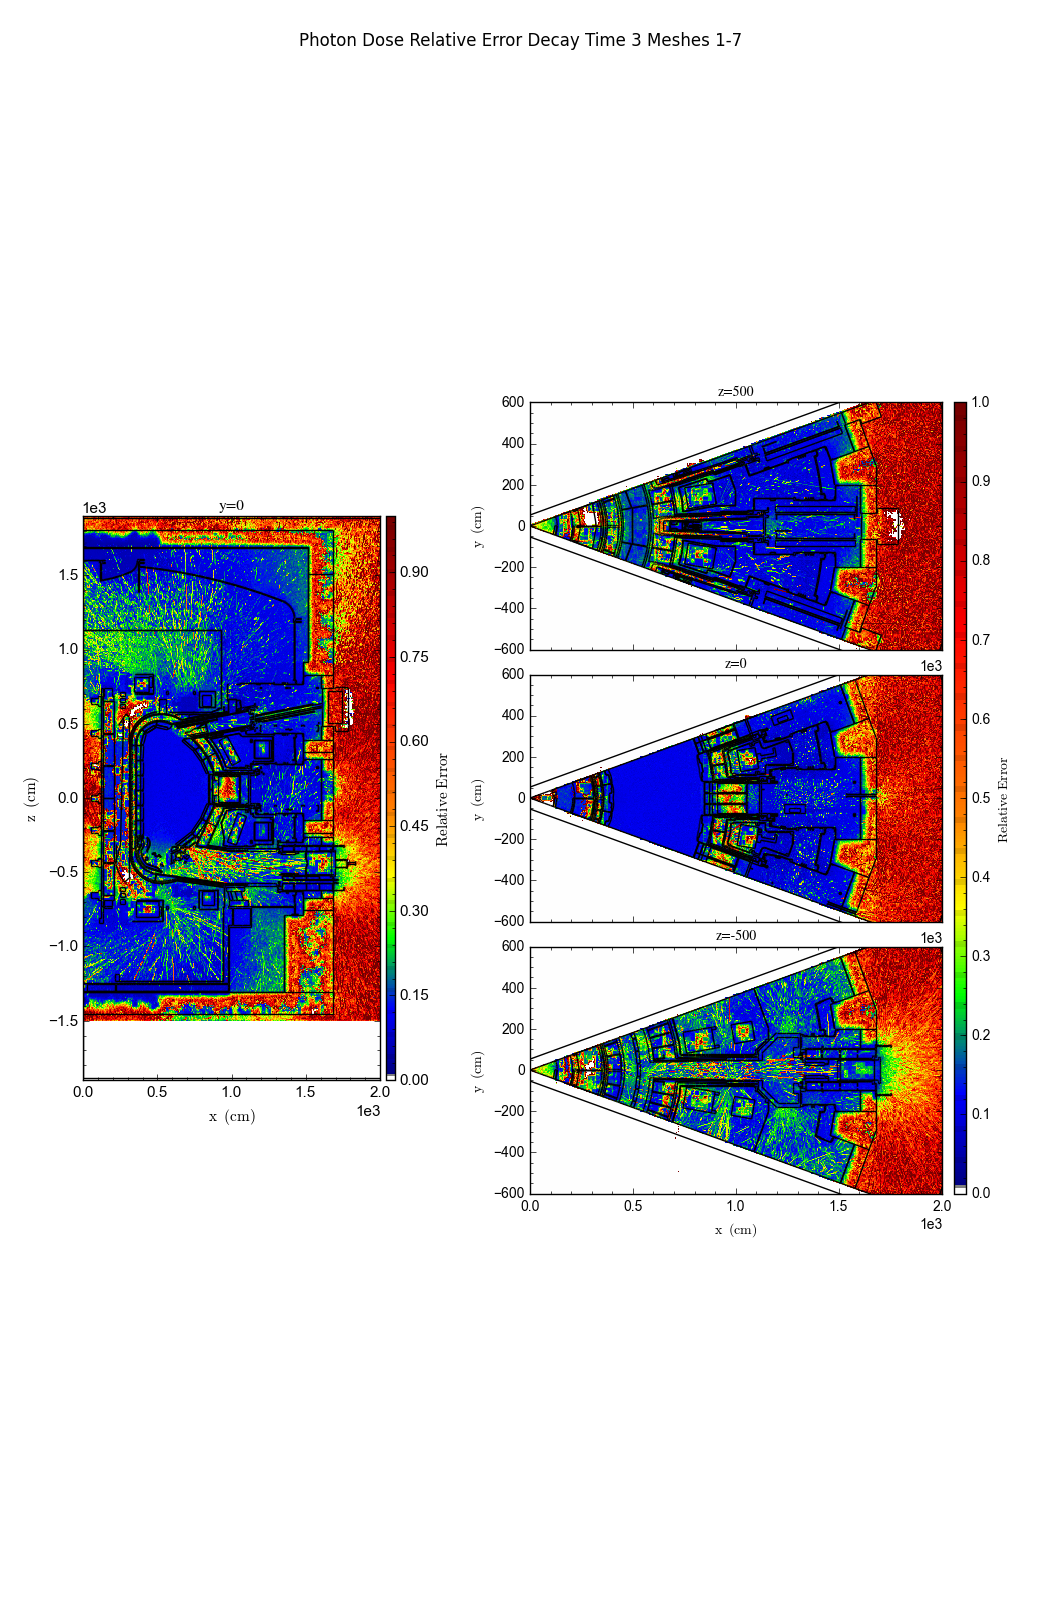
\includegraphics[trim={0cm 8cm, 0cm 8cm},clip,scale=0.75]{../plots/final_model/10year/Photon_Dose_Relative_Error_Decay_Time_3_Meshes_1-7.png}
\caption{Total dose rate relative error for decay time 3 for the 10 year irradiation}
\label{fig:photons_10y_dc3_nob4c_relerr}
\end{figure}

\end{document}
